\documentclass[11pt]{report}


\usepackage[margin=1in]{geometry}  
\usepackage{graphicx}              
\usepackage{amsmath}               
\usepackage{amsfonts}              
\usepackage{amsthm}                
\usepackage{amssymb}
\usepackage{mathrsfs}
\usepackage{url}
\usepackage{subfig}
\usepackage{xfrac}
\usepackage[sectionbib]{chapterbib}
\usepackage{hyperref}
\usepackage{tikz}
\usetikzlibrary{positioning}
\usetikzlibrary{calc}
\usepackage{packages/algorithmic}
\usepackage{packages/seqsplit}
\usepackage{packages/multirow}
\usepackage{pifont}
\usepackage{xcolor}
\usepackage[T1]{fontenc}
\usepackage{libertine}
\usepackage[libertine]{newtxmath}


%//////////////////////////////////////////////////////////////////////////////////////////////////

\definecolor{citecolor}{HTML}{00AA00}
% to make the refrences clickable, and...
\hypersetup{
	unicode = true,
    colorlinks = true,
    citecolor = citecolor,
    filecolor = blue,
    linkcolor = blue,
    urlcolor = blue,
    pdfstartview = {FitH},
}


% theorem environments
\theoremstyle{plain}
\newtheorem{theorem}{Theorem}
\newtheorem{lemma}[theorem]{Lemma}
\newtheorem{corollary}[theorem]{Corollary}
\newtheorem{proposition}[theorem]{Proposition}
\theoremstyle{definition}
\newtheorem{definition}[theorem]{Definition}
\newtheorem{conjecture}[theorem]{Conjecture}
\newtheorem{example}[theorem]{Example}
\newtheorem*{remark}{Remark}
\newtheorem*{note}{Note}
\newenvironment{result}{\par\addvspace{3mm}\ding{96}\hspace*{2mm}\itshape}{\par\addvspace{3mm}}

\renewcommand{\algorithmicrequire}{\textbf{Input:}}
\renewcommand{\algorithmicensure}{\textbf{Output:}}
\algsetup{linenodelimiter=.}

\newcommand{\wrt}{\vdash} 
\newcommand{\ang}[1]{\langle#1\rangle}
\newcommand{\abs}[1]{\left\vert#1\right\vert}
\newcommand{\dual}[1]{\overline{#1}}
\newcommand{\tildO}{\tilde{O}}
% roman numerals
\newcommand{\romnum}[1]{\romannumeral #1}
\newcommand{\Romnum}[1]{\uppercase\expandafter{\romannumeral #1}}



\DeclareMathOperator{\fieldchar}{char} % characteristic of a field
\DeclareMathOperator{\ringofend}{End} % endomorphism ring
\DeclareMathOperator{\trace}{tr} % trace of a mtrix
\DeclareMathOperator{\gal}{Gal} % Galois group
\DeclareMathOperator{\order}{ord} % order of an element
\DeclareMathOperator{\lcm}{lcm} % least common multiple
\DeclareMathOperator{\divisor}{div} % divisor on a curve
\DeclareMathOperator{\supp}{supp} % support of a divisor
\DeclareMathOperator{\norm}{N} % norm
\DeclareMathOperator{\Res}{Res}

\def\Q{\ensuremath{\vmathbb{Q}}}
\def\N{\ensuremath{\vmathbb{N}}}
\def\R{\ensuremath{\vmathbb{R}}}
\def\Z{\ensuremath{\vmathbb{Z}}}
\def\F{\ensuremath{\vmathbb{F}}}
\def\H{\ensuremath{\vmathbb{H}}}
\def\K{\ensuremath{\vmathbb{K}}}
\def\Kbar{\ensuremath{\overline{\vmathbb{K}}}}
\def\L{\ensuremath{\vmathbb{L}}}
\def\A{\ensuremath{\vmathbb{A}}}
\def\B{\ensuremath{\vmathbb{B}}}
\def\MM{\ensuremath{\mathsf{M}}}
\def\II{\ensuremath{\mathsf{I}}}
\def\QQ{\ensuremath{\mathsf{Q}}}
\def\CC{\ensuremath{\mathsf{C}}}
\def\RR{\ensuremath{\mathsf{R}}}
\def\AA{\ensuremath{\mathsf{A}}}
\def\va{\ensuremath{\mathsf{a}}}
\def\vy{\ensuremath{\mathsf{y}}}
\def\vu{\ensuremath{\mathsf{u}}}
\def\vb{\ensuremath{\mathsf{b}}}
\def\vc{\ensuremath{\mathsf{c}}}
\def\mul{\ensuremath{\mathsf{mul}}}
\def\rem{\ensuremath{\mathsf{rem}}}
\def\cat{\ensuremath{\mathsf{cat}}}
\def\coeff{\ensuremath{\mathsf{coefficient}}}
\def\mulmod{\ensuremath{\mathsf{mulmod}}}
\def\rev{\ensuremath{\mathsf{rev}}}
\def\x{\ensuremath{\mathbf{x}}}
\def\uu{\ensuremath{\mathbf{U}}}
\def\bb{\ensuremath{\mathbf{B}}}
\def\bxi{\boldsymbol{\xi}}
\def\bupsilon{\boldsymbol{\upsilon}}
\def\bzeta{\boldsymbol{\zeta}}
\def\blambda{\boldsymbol{\lambda}}


% allow algorithms to split over multiple pages
\makeatletter
\newcounter{algorithm}
\setcounter{algorithm}{0}
\renewcommand{\thealgorithm}{\arabic{algorithm}}
\def\algorithm{\@ifnextchar[{\@algorithma}{\@algorithmb}}
\def\@algorithma[#1]{%
	\refstepcounter{algorithm}
	\trivlist
	\leftmargin\z@
	\itemindent\z@
	\labelsep\z@
	\item[\parbox{\columnwidth}{%
		\hrule
		\hrule
		\noindent\strut\textbf{Algorithm \thealgorithm} #1
		\hrule
	}]\hfil\vskip0em%
}
\def\@algorithmb{\@algorithma[]}
\def\endalgorithm{\hfil\vskip-1em\hrule\endtrivlist}
\makeatother

\setlength{\parindent}{0pt}

% remove chapter gap from list of figures and tables
\newcommand*{\noaddvspace}{\renewcommand*{\addvspace}[1]{}}

\sloppy

\begin{document}
	\pagenumbering{roman}
	\thispagestyle{empty}
\vspace*{1.5in}
\begin{center}
	\LARGE
	\textbf{Computing in Algebraic Closures of \\ Finite Fields} \\
	\normalsize
	\bigskip
	(Thesis format:  Integrated-Article)\\
	\smallskip
	\textbf{Javad Doliskani}\\
	\vspace*{1in}
	Department of Computer Science\\
	\vspace*{0.3in}
	A thesis submitted in partial fulfillment\\
	of the requirements for the degree of\\
	Doctor of Philosophy\\
	\vspace*{0.3in}
	The School of Graduate and Postdoctoral Studies\\
	The University of Western Ontario\\
	London, Ontario, Canada\\
	\vfill
	\copyright \hspace*{0.07in} J. Doliskani 2016  \\
\end{center}

	
\vspace*{2in}
\begin{center}
	\large
	\textbf{Abstract}
\end{center}
\vspace*{1cm}

We present algorithms to construct and perform computations in algebraic closures of finite 
fields. Inspired by algorithms for constructing irreducible polynomials, our approach for 
constructing closures consists of two phases; First, extension towers of prime power degree are 
built, and then they are glued together using composita techniques. To be able to move elements 
around in the closure we give efficient algorithms for computing isomorphisms and embeddings. In 
most cases, our algorithms which are based on polynomial arithmetic, rather than linear algebra, 
have quasi-linear complexity.
 
\vspace*{1cm}
\begin{description}
	\item[Keywords:] Algebraic closure, polynomial arithmetic, finite field.
\end{description}
	
\vspace*{2in}
\begin{center}
	\large
	\textbf{Co-Authorship} \\
\end{center}
\vspace*{2cm}

This document is based on the following joint works with \'{E}ric Schost and Luca Defeo.
\begin{description}
	\item[Chapter \ref{chapter:high-ext-roots}] Taking roots over high extensions of finite 
	fields. \textit{Mathematics of Computation}, 83(285), pp. 435-446, 2014.
	\item[Chapter \ref{chapter:2ext-op}] Computing in degree 2k-extensions of finite fields of 
	odd characteristic. \textit{Des. Codes Cryptography}, 74(3), pp. 559-569, 2015.
	\item[Chapter \ref{chapter:ell-adic}] Fast algorithms for $\ell$-adic towers over finite 
	fields. 
	\textit{In Proceedings of the 38th International Symposium on Symbolic and Algebraic 
	Computation (ISSAC'13)}. ACM, New York, NY, USA.
	\item[Chapter \ref{chapter:alg-closure}] Fast arithmetic for the algebraic closure of finite 
	fields. \textit{In Proceedings of the 39th International Symposium on Symbolic and Algebraic 
	Computation (ISSAC '14)}, ACM, New York, NY, USA.
\end{description}

	\addtocontents{lot}{\protect\noaddvspace}
	\addtocontents{lof}{\protect\noaddvspace}
	\listoftables
	\listoffigures
	\tableofcontents
	\pagenumbering{arabic}
	\graphicspath{{introduction/}}

\chapter{Introduction}

The theory of finite fields has found much attention during recent decades, most notably due to 
developments in the branches of computer science such as cryptography, coding theory, switching 
circuits, and combinatorics \cite{lidl2012applied}. In applications, one almost always encounters 
finite fields that are extensions of the so-called prime fields. For example, in public-key 
cryptography, there are cryptosystems that are based on the group of points on an algebraic curve. 
To have a secure system one must go through the process of choosing a random secure curve. A good 
class of candidates for such curves are hyperelliptic curves. One of the efficient methods of 
choosing a secure hyperelliptic curve requires counting the number of points on the curve, which in 
turn requires building a large number of successive extensions over a small prime field 
\cite{df10, GaSc12}. 

The natural need for extensions usually arises from the need for manipulating polynomials and their 
roots. Once the extension are built, the next step is to be able to move elements from one 
extension to the other. This is where algebraic closures come to the fore. From a computational 
point of view, an algebraic closure of a given field can be seen as a large enough finite extension 
that contains the roots of a given finite set of polynomials. Computation in algebraic closures 
has been considered by others, e.g. \cite{Steel2010342} and references therein. In this chapter, we 
briefly review some basic properties of finite fields, and discuss some notations on the running 
time complexities of some basic arithmetics over them. At the end, we give an overview of our 
computational approach to algebraic closures.


\section{Notations}

In this section, we give a very brief review of finite fields concepts and notations used in the 
subsequent chapters. For a more detailed preliminary on finites fields we refer the reader to 
Appendix \ref{appendix:finite_fields}. Given a prime number $p$, we denote the prime finite field 
with $p$ elements by $\F_p$. The prime number $p$ is called the characteristic of the field. 

\paragraph{Irreducible polynomials.}
The univariate polynomial ring over $\F_p$ is denoted by $\F_p[X]$. The elements of $\F_p[x]$ are 
of the form $f(X) = a_{n}X^n + a^{n - 1}X^{n - 1} + \cdots + a_0$ where $a_i \in \F_p$. The degree 
of $f$, denoted by $\deg f$, is $n$. We call $f$ monic if its leading coefficient $a_n$ is 1. The 
division and remainder operation in $\F_p[X]$ is done using the usual polynomial arithmetic. A 
polynomial $f \in \F_p[X]$ is reducible if it can be written as $f = gh$ for polynomials $g, h \in 
\F_p[X]$ of degree $> 0$; otherwise it is called \textit{irreducible}. For a monic irreducible 
polynomials $f$ of degree $n$ the quotient $\F_p[X] / \ang{f}$ is a finite field extension of 
$\F_p$ of degree $n$. We usually denote such an extension by $\F_q$ where $q = p^n$.  

\paragraph{Operation complexities}
The nature of the algorithms presented in this document suggests an algebraic complexity model. 
This means we will count operations $\{+, -, \times, \div \}$ in a based field such as $\F_p$ or 
$\F_q$. Consequently, we have to choose a representation for elements of field extensions. For 
example, one could proceed implementing algorithms using normal basis representation, in which 
case the complexity estimates are stated differently. However, we shall use the monomial basis 
representation, since in particular our implementations and result comparisons are based on 
systems such as NTL \cite{shoup2003ntl}, Magma \cite{MAGMA}, and FLINT \cite{hart2010flint}. In 
the monomial representation, the finite field or even ring extension are represented by quotients. 
For example, the finite field $\F_{q^n}$ is represented by $\F_q[X] / \ang{f}$ where $f$ is a 
monic irreducible polynomial of degree $n$ in $\F_q[X]$. So an element $a \in \F_{q^n}$ is a 
polynomial of degree less than $n$ in $\F_q[X]$. 

One of the most fundamental operations in all algebraic systems is \textit{polynomial 
multiplication}. We denote the upper bound for the cost of multiplying two polynomials of degree 
$n$ by $\MM(n)$. This means for a given field $K$ and two polynomials $f, g \in K[X]$ of degree 
$n$, $fg$ can be computed using $\MM(n)$ multiplications in $K$. The best known upper bound for 
$\MM(n)$ is $O(n\log(n)\log\log(n))$ \cite{Schonhage1971,CaKa91}. This is done using Fast Fourier 
Transform. The idea is to reduce the polynomial multiplication to point-wise vector-vector 
multiplication using an invertible change of representation. See \cite[Chapter~8]{GaGe03} for more 
details. We assume that $\MM(n)$ is a super-linear function, i.e. not bounded by any linear 
function.

Another fundamental operation is \textit{matrix multiplication}. Given two square matrices of size 
$n$ over a field $K$ we assume they can be multiplied using $O(n^\omega)$ multiplications in $K$, 
where $\omega$ is called the linear algebra exponent. A naive implementation would give $\omega = 
3$. A slightly better algorithm due to Strassen \cite{Strassen1969} gives a bound $\omega \le 2.81$.
The algorithm uses a divide and conquer approach to reduce the multiplication problem to sub-blocks 
of the given matrices. The smallest known bound is $\omega \le 2.37$ due to Coppersmith and 
Winograd \cite{CoWi90}. 

Given polynomials $f, g, h \in K[X]$ of degree $n$, the \textit{modular composition} problem is to 
compute $f(g) \mod{h}$. We denote the upper bound for modular composition by $\CC(n)$. In a boolean 
complexity model, in which bit or word operation are counted, there is an algorithm due to 
Kedlaya and Umans \cite{KeUm11, Umans08} that runs in $O(n^{1+\varepsilon}\log(p)^{1+o(1)})$ 
operations. Since we do not follow a boolean model, and there is still no competitive  
implementation of their algorithm that we know of, we opt for the well-known algorithm of Brent and 
Kung \cite{BrKu78}. Their algorithm gives the bound $O(n^{(\omega+1)/2})$. We can take $\omega \le 
2.37$ using the Coppersmith and Winograd algorithm which gives $\CC(n)=O(n^{1.69})$. There is the 
slightly better bound $\CC(n)=O(n^{1.67})$ due to Pan \cite{HuPa98}, which uses rectangular matrix 
multiplication.

\paragraph{Algebraic closures.}
A field extension $K \subseteq L$ is said to be algebraic if every element $a \in L$ is a root of a 
monic polynomial in $K[X]$. A field $K$ is algebraically closed if $L = K$ for every algebraic 
extension of $L$. An algebraic closure of a field $K$, denoted by $\overline{K}$, is an 
algebraically closed algebraic extension of $K$. 

Let $E, F$ be extensions of $K$. Assume that $E, F$ are contained in some larger field $L$. We 
define the \textit{compositum} of $E, F$, denoted by $EF$, to be the smallest subfield of $L$ 
containing both $E, F$. Generally, we can define the compositum of a family $\{ F_i \}_{i \in I}$ 
of subfields of $L$ to be the smallest subfield of $L$ containing all $F_i$. The compositum of $E, 
F$ is not defined unless we have embeddings of both fields into a common field $L$. Let $m = [E: 
K]$ and $n = [F: K]$. We have the following diagram of extensions:
\begin{center}
	\begin{tikzpicture}[node distance = 2cm]
		\node (L) {$L$};
		\node[below = 1cm of L] (EF) {$EF$};
		\node[below left of = EF] (E) {$E$};
		\node[below right of = EF] (F) {$F$};
		\node[below right of = E] (K) {$K$};
		\draw (L) edge (EF);
		\draw (EF) edge node[above left] {$\le n$} (E) edge node[above right] {$\le m$} (F);
		\draw (K) edge node[below left] {$m$} (E) edge node[below right] {$n$} (F);
	\end{tikzpicture}
\end{center}
From the diagram $[EF: K] \le mn$ and $m \mid [EF: K]$ and $n \mid [EF: K]$. So if $\gcd(m, n) = 1$ 
then $[EF: K] = mn$. Therefore, if $E, F$ are finite fields $\F_{p^n}, \F_{p^m}$ with $\gcd(m, n) = 
1$ then the compositum $EF$ is the finite field $\F_{p^{mn}}$. This allows us to define the 
algebraic closure of $\F_p$ as the union
\[ \overline{\F_p} = \bigcup_{i \ge 1} \F_{p^i}. \]


\section{Our approach}

Let $\F_q$ be a finite field with $q = p^n$ a prime power. We divide the construction of 
$\overline{\F_q}$ into two major steps: building towers, and gluing towers. Let us explain what 
these mean. Let $\ell$ be a prime number, and let 
\[ \F_q \subset \F_{q^\ell} \subset \F_{q^{\ell^2}} \subset \cdots \]
a sequence of extensions each of degree $\ell$. We call this an \emph{$\ell$-adic tower}. Define 
the \emph{$\ell$-adic closure} of $\F_q$ to be the union
\[ \F_q^{(\ell)} = \bigcup_{i\ge 0}\F_{q^{\ell^i}}. \]
Assume we have build these towers for different prime $\ell$. Then we can glue them together to get 
the algebraic closure. By gluing here we mean computing composita. Figure \ref{figure:alg-closure}  
shows the above structure of $\overline{\F_q}$. The solid circles in the middle are the composita.
\begin{figure}
	\begin{center}
		\tikzset{
			dotstyle/.style={inner sep = 2pt, outer sep = 2pt, circle, fill = lightgray},
			edgetower/.style={thick},
			edgecomp/.style={thick, lightgray}
		}
		\begin{tikzpicture} %, every node/.style={inner sep = 2pt, scale=0.8}]
			\coordinate (T2) at (-2, 0.5);
			\node (Fq) at (0, 0) {$\F_q$};
			\node (Fq2) at ($(Fq) + (T2)$) {$\F_{q^2}$};
			\node (Fq4) at ($(Fq2) + (T2)$) {$\F_{q^4}$};
			\node (Fq2l) at ($(Fq4) + (T2)$) {$\F_q^{(2)}$};
			%---------------------
			\coordinate (T3) at (-0.7, 2);
			\node (Fq3) at ($(Fq) + (T3)$) {$\F_{q^3}$};
			\node (Fq9) at ($(Fq3) + (T3)$) {$\F_{q^9}$};
			\node (Fq3l) at ($(Fq9) + (T3)$) {$\F_q^{(3)}$};
			%---------------------
			\coordinate (T5) at (0.7, 2);
			\node (Fq5) at ($(Fq) + (T5)$) {$\F_{q^5}$};
			\node (Fq25) at ($(Fq5) + (T5)$) {$\F_{q^{25}}$};
			\node (Fq5l) at ($(Fq25) + (T5)$) {$\F_q^{(5)}$};
			%---------------------
			\coordinate (Tl) at (2, 1);
			\node[blue] (Fql) at ($(Fq) + (Tl)$) {$\F_{q^\ell}$};
			\node[blue] (Fql2) at ($(Fql) + (Tl)$) {$\F_{q^{\ell^2}}$};
			\node[blue] (Fqll) at ($(Fql2) + (Tl)$) {$\F_q^{(\ell)}$};
			%---------------------
			\node[dotstyle] (dot1) at ($(Fq2) + (Fq3) - (Fq)$){};
			\node[dotstyle] (dot2) at ($(Fq4) + (dot1) - (Fq2)$){};
			\node[dotstyle] (dot3) at ($(Fq2) + (Fq5) - (Fq)$){};
			\node[dotstyle] (dot4) at ($(Fq3) + (Fq5) - (Fq)$){};
			\node[dotstyle] (dot5) at ($(Fq3) + (Fql) - (Fq)$){};
			\node[dotstyle] (dot6) at ($(Fq5) + (Fql) - (Fq)$){};
			%---------------------
			\draw 
			(Fq) 
			edge[edgetower] (Fq2)
			edge[edgetower] (Fq3)
			edge[edgetower] (Fq5)
			edge[edgetower, blue] (Fql)
			(Fq2)
			edge[edgetower] (Fq4)
			edge[edgecomp] (dot1)
			(Fq4)
			edge[edgetower, dotted] (Fq2l)
			edge[edgecomp] (dot2)
			(dot1)
			edge[edgecomp] (dot2)
			(Fq3)
			edge[edgetower] (Fq9)
			edge[edgecomp] (dot1)
			edge[edgecomp] (dot4)
			(Fq9)
			edge[edgetower, dotted] (Fq3l)
			(Fq5)
			edge[edgetower] (Fq25)
			edge[edgecomp] (dot4)
			edge[edgecomp] (dot6)
			(Fq25)
			edge[edgetower, dotted] (Fq5l)
			(Fql)
			edge[edgetower, blue] (Fql2)
			edge[edgecomp] (dot6)
			(Fql2)
			edge[edgetower, blue, dotted] (Fqll)
			(dot3)
			edge[edgecomp] (Fq2)
			edge[edgecomp] (Fq5)
			(dot5)
			edge[edgecomp] (Fq3)
			edge[edgecomp] (Fql);
		\end{tikzpicture}
	\end{center}
	\caption{Algebraic closure of $\F_q$}
	\label{figure:alg-closure}
\end{figure}

\paragraph{$\ell$-adic towers.} Let $F_i = \F_{q^{\ell^i}}$ be the level $i$ of the $\ell$-adic 
tower for an integer $i > 0$. The goal is to be able to compute in $F_i$ in quasi-linear time in 
the extension degree $\ell^i$. For this we need first to construct the tower, and then be able to 
move up and down to different levels of the tower efficiently. 

In many cases, building extensions and isomorphisms of finite fields requires taking roots of 
elements. In Chapter \ref{chapter:high-ext-roots} we discuss taking arbitrary roots over extensions 
of finite fields. The idea is to reduce the problem to root extraction in subfields using 
trace-like computations. For example, using our algorithm, the complexity of taking square roots in 
$\F_q$ is an expected $O(\MM(n)\log(p) + \CC(n)\log(n))$ operations in $\F_p$. Computing roots in 
finite fields was previously considered by others like Cipolla \cite{Williams72} and Tonelli-Shanks 
\cite{Shanks1972}. Kaltofen and Shoup \cite{KaltofenShoup1997} give an Equal Degree Factorization 
(EDF) algorithm that can be used for computing roots.

The case $\ell = 2$ of the $\ell$-adic towers, which is of particular interest, is treated 
separately in Chapter \ref{chapter:2ext-op}. Our algorithms presented there for construction of the 
tower and performing basic operations inside the tower are all quasi-linear time. The following 
table summarizes the complexities of our algorithms for some well-known operations for this case.

\begin{center}
	\begin{tabular}{c|c}
		Operation & Cost \\
		\hline
		addition / subtraction & $O(n)$\\
		multiplication & $\MM(n)+O(n)$\\
		inversion & $O(\MM(n))$\\
		quadratic residuosity & $O(\MM(n)+\log(q))$ \\
		square root &  $O(\MM(n)\log(nq))$\ \ (expected) \\
		isomorphism &  $O(n + \log(n)\log(q))$\ \ (expected)
	\end{tabular}
\end{center}
Note the improvement of the square root complexity here compared to the one for general finite 
fields which has a $\CC(n)$ term. Another special case of the $\ell$-adic towers is $\ell = p$, 
called the Artin-Schreier tower. The algorithms for this case were presented in \cite{DeSc12}.

Chapter \ref{chapter:ell-adic} discusses the towers for a general $\ell$. The field 
$\F_{q^{\ell^i}}$ can be represented by two natural bases over $\F_q$. For a univariate 
representation of the form $\F_q[X_i]/\ang{Q_i}$, where $Q_i \in \F_q[X_i]$ is a monic irreducible 
polynomial of degree $\ell^i$, we get the monomial basis
\[ \uu_i = (1,x_{i},x_{i}^2,\ldots,x_{i}^{\ell^{i}-1}) \] 
for $\F_{q^{\ell^i}}$ over $\F_q$. Here $x_i$ is the residue class of $X_i$ modulo $Q_i$. But we 
can also consider $\F_{q^{\ell^i}}$ as a degree $\ell$ extension over $\F_{q^{\ell^{i - 1}}}$, 
i.e. as a bivariate quotient
\[ \F_q[X_{i-1},X_i]/\ang{Q_{i-1}(X_{i-1}), T_i(X_{i-1},X_i)} \]
where $T_i$ is a monic polynomial of degree $\ell$ in $X_i$, and of degree less than $\ell^{i-1}$ 
in $X_{i-1}$. This gives the basis
\[ \bb_{i} = (1,\ldots,x_{i-1}^{\ell^{i-1}-1},\ldots,x_i^{\ell-1},\ldots, x_{i-1}^{\ell^{i-1}-1}
x_i^{\ell-1}). \]
for $\F_{q^{\ell^i}}$ over $\F_q$. The complexity of constructing the tower, which requires some 
initialization and finding $Q_i, T_i$, is close to quasi-linear. Using the usual algorithms, basic 
operations like multiplication and inversion in $\F_q[X_i]/\ang{Q_i}$ are done using respectively 
$O(\MM(\ell^i))$ and $O(\MM(\ell^i)\log(\ell^i))$ operations in $\F_q$. These are quasi-linear in 
the extension degree $\ell^i$. Moving up and down in the tower is done using repeated applications 
of two operations called \textit{lift} and \textit{push}. Lifting refers to the change of basis 
from $\bb_i$ to $\uu_i$ while pushing is the inverse transformation. These operations are also 
very close to being quasi-linear. The following table summarizes our main complexity results.

\vspace*{4mm}
\resizebox{\textwidth}{!}{$
	\def\arraystretch{1.2}
	\begin{array}{c|cccc}
		\text{Condition} & \text{Initialization} & Q_i, T_i & \text{Lift, push}\\
		\hline \hline
		q = 1 \bmod \ell & O_e(\log(q))  & O(\ell^i) & O(\ell^i) \\
		q = -1 \bmod \ell & O_e(\log(q)) & O(\ell^i) & O(\MM(\ell^i) \log(\ell^i)) \\
		- & O_e (\ell^2+\MM(\ell) \log(q)) & O(\MM(\ell^{i+1})\MM(\ell)\log(\ell^i)^2) & O( 
		\MM(\ell^{i+1})\MM(\ell)\log(\ell^i))\\
		4\ell \le q^{\sfrac{1}{4}} & O\tilde{_e}(\ell\log^5(q)+\ell^3) \text{~(bit)}  & 
		O_e(\ell^2+\MM(\ell)\log(\ell
		q)+\MM(\ell^i)\log(\ell^i)) & O(\MM(\ell^i) \log(\ell^i)) \\
		4\ell \le q^{\sfrac{1}{4}} & O\tilde{_e}(\ell\log^5(q))  \text{~(bit)}  + 
		O_e(\MM(\ell)\sqrt{q}\log(q)) & O_e(\log(q) + \MM(\ell^i) \log(\ell^i)) & O(\MM(\ell^i) 
		\log(\ell^i))
	\end{array}
$}

\vspace*{4mm}
The probabilistic complexities with expected running time are denoted by $O_e(\ )$. Also
$O\tilde{_e}(\ )$ indicates the additional omission of logarithmic factors. Although in some cases 
there are extra factors of $\ell$, we have achieved quasi-linear time in the degree of the 
extension $\ell^i$ in most of the cases. Our algorithm for constructing towers are inspired by the
previous works of Shoup \cite{Shoup90,shoup94} and Lenstra / De Smit 
\cite{lenstra+desmit08-stdmodels}, and Couveignes / Lercier \cite{couveignes+lercier11}. See the 
introduction of Chapter \ref{chapter:ell-adic} for more details.

\paragraph{Composita.} In Chapter \ref{chapter:alg-closure}, we discuss the composita of fields. 
Let $\F_{p^m} = \F_p[x] / \ang{Q_m(x)}$ and $\F_{p^n} = \F_p[y] / \ang{Q_n(y)}$ be two finite 
fields where $Q_m(x) \in \F_p[x]$ and $Q_n(y) \in \F_p[y]$ are irreducible of comprime degrees $m, 
n > 1$ respectively. Define the \textit{composed product} of $Q_m, Q_n$ as
\[ Q_{mn}(z) = \prod_{\substack{1 \le i \le m \\ 1 \le j \le n}} (z- a_i b_j) \]
where $(a_i)_{1 \le i \le m}$ and $(b_j)_{1 \le j \le n}$ are roots of $Q_m$ and $Q_n$ in the 
algebraic closure of $\F_p$. The polynomial $Q_{mn}$ is irreducible of degree $mn$ in $\F_p[z]$, 
see \cite{Brawley1987}. The field $\F_p[z] / \ang{Q_{mn}(z)}$ is the compositum of $\F_{p^m}$ and 
$\F_{p^n}$, and there exists embeddings $\varphi_x$, $\varphi_y$, and an isomorphism $\Phi$ of the 
form
$$
\begin{array}{rrll}
\varphi_x: & \F_p[x]/\ang{Q_m} & \to & \F_p[z]/\ang{Q_{mn}},\\
\varphi_y: & \F_p[y]/\ang{Q_n} & \to & \F_p[z]/\ang{Q_{mn}},\\
\Phi:&  A=\F_p[x,y]/\ang{Q_m,Q_n} & \to & \F_p[z]/\ang{Q_{mn}} \\
&  xy & \mapsfrom & z.
\end{array}$$
The goal is to compute $\varphi_x$, $\varphi_y$, and $\Phi$ and $\Phi^{-1}$ efficiently. We present 
algorithms for computing $\varphi_x$ and $\varphi_y$ which run using $O(n\MM(m)+m\MM(n))$ 
operations in $\F_p$. Assuming that $m \le n$, $\Phi$ and $\Phi^{-1}$ can be computed using either 
$O(m^2 \MM(n))$ or $O(\MM(mn)n^{1/2}+\MM(m)n^{(\omega+1)/2} )$ operations in $\F_p$ where $\omega$ 
is the linear algebra exponent. Therefore, computing embeddings $\varphi_x, \varphi_y$ is 
quasi-linear in $mn$ while computing the isomorphisms $\Phi, \Phi^{-1}$ has an extra factor of $m$ 
or $n$. Previous algorithms such as the ones presented in \cite{bosma+cannon+steel97}, and 
\cite{LenstraJr91,Allombert02} also compute embeddings of finite fields. They rely on linear 
algebra which results in complexities at least quadratic in the degree of the extensions.

\bibliographystyle{plain}
\bibliography{references}
	\graphicspath{{roots_high_ext/}}

\chapter{Taking Roots over High Extensions of Finite Fields}
\label{chapter:high-ext-roots}

\section{Introduction}\label{section:intro}

Beside its intrinsic interest, computing $m$-th roots over finite
fields (for $m$ an integer at least equal to $2$) has found many
applications in computer science. Our own interest comes from elliptic
and hyperelliptic curve cryptography; there, square root computations
show up in pairing-based cryptography~\cite{BaKiLySc02} or
point-counting problems~\cite{GaSc10}.


Our result in this paper is a new algorithm for computing $m$-th roots
in a degree $n$ extension $\F_q$ of the prime field $\F_p$, with $p$ a
prime. Our emphasis is on the case where $p$ is thought to be small,
and the degree $n$ grows. Roughly speaking, we reduce the problem to
$m$-th root extraction in a lower degree extension of $\F_p$ (when
$m=2$, we actually reduce the problem to square root extraction over
$\F_p$ itself).

% multiplications and exponentiations by powers of $p$ in $\F_q$, a
% $t$-th root extraction in $\F_p$, and a few other operations.

\paragraph{Our complexity model.}
It is possible to describe the algorithm in an abstract manner,
independently of the choice of a basis of $\F_q$ over $\F_p$. However,
to give concrete complexity estimates, we have to decide which
representation we use, the most usual choices being monomial and
normal bases. We choose to use a monomial basis, since in particular
our implementation is based on the library NTL~\cite{NTL2009}, which
uses this representation.  Thus, the finite field $\F_q=\F_{p^n}$ is
represented as $\F_p[X]/\langle f\rangle$, for some monic irreducible
polynomial $f \in \F_p[X]$ of degree $n$; elements of $\F_q$ are
represented as polynomials in $\F_p[X]$ of degree less than $n$. We
will briefly mention the normal basis representation later on.

The costs of all algorithms are measured in number of operations
$+,\times,\div$ in the base field $\F_p$ (that is, we are using an
algebraic complexity model) --- at the end of this introduction, we
discuss how our results can be stated in the boolean model, in light
especially of results by Umans~\cite{Umans08} and Kedlaya and
Umans~\cite{KeUm11}.

We shall denote upper bounds for the cost of {\em polynomial
  multiplication} and {\em modular composition} by respectively
$\MM(n)$ and $\CC(n)$. This means that over any field $\K$, we can
multiply polynomials of degree $n$ in $\K[X]$ in $\MM(n)$ base field
operations, and that we can compute $f(g) \bmod h$ in $\CC(n)$
operations in $\K$, when $f,g,h$ are degree $n$ polynomials. We
additionally require that both $\MM$ and $\CC$ are super-linear
functions, as in~\cite[Chapter~8]{GaGe03}, and that $\MM(n)=O(\CC(n))$.
In particular, since we work in the monomial basis, multiplications
and inversions in $\F_q$ can be done in respectively $O(\MM(n))$ and
$O(\MM(n)\log(n))$ operations in $\F_p$, see again~\cite{GaGe03}.

The best known bound for $\MM(n)$ is $O(n\log(n)\log\log(n))$, achieved
by using Fast Fourier Transform~\cite{Schonhage1971,CaKa91}.  The most
well-known bound for $\CC(n)$ is $O(n^{(\omega+1)/2})$, due to Brent
and Kung~\cite{BrKu78}, where $\omega$ is such that matrices of size
$n$ over any field $\K$ can be multiplied in $O(n^\omega)$ operations
in $\K$; this estimate assumes that $\omega > 2$, otherwise some
logarithmic terms may appear. Using the algorithm of Coppersmith and
Winograd~\cite{CoWi90}, we can take $\omega \le 2.37$ and thus
$\CC(n)=O(n^{1.69})$; an algorithm by Huang and Pan~\cite{HuPa98}
actually achieves a slightly better exponent of $1.67$, by means of
rectangular matrix multiplication.

\paragraph{Main result.}
We will focus in this paper on the case of $t$-th root extraction,
where $t$ is a prime divisor of $q-1$; the general case of $m$-th root
extraction, with $m$ arbitrary, can easily be reduced to this case
(see the discussion after Theorem~\ref{theo:main}).

The core of our algorithm is a reduction of $t$-th root extraction in
$\F_q$ to $t$-th root extraction in an extension of $\F_p$ of smaller
degree. Our algorithm is probabilistic of Las Vegas type, so 
its running time is given as an expected number of operations. With
this convention, our main result is the following.

\begin{theorem}\label{theo:main}
  Let $t$ be a prime factor of $q-1$, with $q=p^n$, and let $s$ be the
  order of $p$ in $\vmathbb{Z}/t\vmathbb{Z}$. Given $a\in \F_q^*$, one
  can decide if $a$ is a $t$-th power in $\F_q^*$, and if so compute
  one of its $t$-th roots, by means of the following operations:
  \begin{itemize}
  \item an expected $O(s\MM(n)\log(p) + \CC(n)\log(n))$ operations in
    $\F_p$;
  \item a $t$-th root extraction in $\F_{p^s}$.
  \end{itemize}
\end{theorem}

Thus, we replace $t$-th root extraction in a degree $n$ extension by a
$t$-th root extraction in an extension of degree $s \le \min(n,t)$.
The extension degree $s$ is the largest one for which $t$ still
divides $p^s-1$, so iterating the process does not bring any
improvement: the $t$-th root extraction in $\F_{p^s}$ must be dealt
with by another algorithm. The smaller $s$ is, the better.

A useful special case is $t=2$, that is, we are taking square roots;
the assumption that $t$ divides $q-1$ is then satisfied for all odd
primes $p$ and all $n$. In this case, we have $s=1$, so the second
step amounts to square root extraction in $\F_p$. Since this can be
done in $O(\log(p))$ expected operations in $\F_p$, the total running
time of the algorithm is an expected $O(\MM(n)\log(p) + \CC(n)\log(n))$
operations in $\F_p$. 

A previous algorithm by Kaltofen and Shoup~\cite{KaltofenShoup1997}
allows one to compute $t$-th roots in $\F_{p^n}$ in expected time
$O((\MM(t)\MM(n)\log(p) + t \CC(n) + \CC(t)\MM(n))\log(n))$; we discuss
it further in the next section. This algorithm requires no assumption
on $t$, so it can be used in our algorithm in the case $s > 1$, for
$t$-th root extraction in $\F_{p^s}$. Then, its expected running time
is $O((\MM(t)\MM(s)\log(p) + t \CC(s) + \CC(t)\MM(s))\log(s))$.

The strategy of using Theorem~\ref{theo:main} to reduce from $\F_q$ to
$\F_{p^s}$ then using the Kaltofen-Shoup algorithm over $\F_{p^s}$
is never more expensive than using the Kaltofen-Shoup algorithm
directly over $\F_{q}$. For $t=O(1)$, both strategies are within a
constant factor; but even for the smallest case $t=2$, our algorithm
has advantages (as explained in the last section). For larger $t$, the
gap in our favor will increase for cases when $s$ is small (such 
as when $t$ divides $p-1$, corresponding to $s=1$).

\medskip

Finally, let us go back to the remark above, that for any $m$, one can
reduce $m$-th root extraction of $a \in \F_q^*$ to computing $t$-th
roots, with $t$ dividing $q-1$; this is well known, see for
instance~\cite[Chapter~7.3]{BachSh1996}. We write $m = uv$ with $(v, q
- 1) = 1$ and $t \mid q - 1$ for every prime divisor $t$ of $u$, and
we assume that $a$ is indeed an $m$-th power.
\begin{itemize}
\item We first compute the $v$-th root $a_0$ of $a$ as
  $a_0=a^{v^{-1} \bmod q - 1}$ by computing the inverse $\ell$ of
  $v \bmod q-1$, and computing an $\ell$-th power in $\F_q$. This
  takes $O(n\MM(n)\log(p))$ operations in $\F_p$.
\item Let $u = \prod_{i = 1}^d{m_i^{\alpha_i}}$ be the prime
  factorization of $u$, which we assume is given to us. Then, for $k =
  1, \dots, \alpha_1$, we compute an $m_1$-th root $a_k$ of $a_{k-1}$
  using Theorem~\ref{theo:main}, so that $a_{\alpha_1}$ is an
  $m_1^{\alpha_1}$-th root of $a_0$.

  One should be careful in the choice of the $m_1$-th roots (which are
  not unique), so as to ensure that each $a_k$ is indeed an
  $u/m_1^i$-th power: if the given $a_k$ is not such a power, we can
  multiply it by a $m_1$-th root of unity until we find a suitable
  one.  The root of unity can be found by the algorithm of
  Theorem~\ref{theo:main}.

  Once we know $a_{\alpha_1}$, the same process can be applied to
  compute an $m_2^{\alpha_2}$-th root of $a_{\alpha_1}$, and so on.
\end{itemize}

The first step, taking a root of order $v$, may actually be the
bottleneck of this scheme. When $v$ is small compared to $n$, it may
be better to use here as well the algorithm by Kaltofen and Shoup
mentioned above.

%Using the $O\tilde{~}$ notation to indicate the omission of
%logarithmic factors and taking $\omega=2$ in the estimates for modular
%composition, this is $O\tilde{~}((t+n)\log(p) + n^2)$. Taking
%$\omega\le 2.37$, this becomes $O\tilde{~}((t+n)\log(p) + n^{1.69})$;
%this is the best result we are aware of for this question.

\paragraph{In a boolean model.} In our algebraic model, when $n$ grows, 
the bottleneck of our algorithm (or of the Kaltofen-Shoup algorithm)
is modular composition, since there is currently no known algorithm
with cost quasi-linear in $n$.

If we analyze running times in a boolean model (counting bit or word
operations), much better can be done: Kedlaya and Umans~\cite{KeUm11},
following previous work by Umans~\cite{Umans08}, give an algorithm
with a boolean cost that grows like $n^{1+\varepsilon}
\log(p)^{1+o(1)}$ for modular composition in degree $n$ over $\F_p$,
for any given $\varepsilon > 0$. They also show that minimal polynomial
of elements of $\F_q=\F_{p^n}$ can be computed for the same cost.

The algorithms of the following sections can be analyzed in the
boolean model without difficulty (for definiteness, over a boolean RAM
with logarithmic access cost --- the Kedlaya-Umans algorithm uses
table lookup in large tables). The only differences are in the cost of
modular composition over $\F_p$, as well as minimal polynomial
computation in $\F_q$, for which we use the results by Kedlaya and
Umans. Using the fact that arithmetic in $\F_p$ can be done in boolean
time $\log(p)^{1+o(1)}$, the running time reported in
Theorem~\ref{theo:main} then becomes $O(s \MM(n)\log(p)^{2+o(1)} +
n^{1+\varepsilon}\log(p)^{1+o(1)})$ bit operations, for any
$\varepsilon > 0$; this admits the upper bound
$O(sn^{1+\varepsilon}\log(p)^{2+o(1)})$. With respect to the extension
degree $n$, this is close to being linear time.

From the practical point of view, however, we did not use the
Kedlaya-Umans algorithm in our experiments, since we do not have a
competitive implementation of it (and currently know of no such
implementation).

\paragraph{Organization of the chapter.} 
The next section reviews and discusses known algorithms;
Section~\ref{section:newRootEx} gives the details of the root
extraction algorithm and some experimental results. In all the paper,
$(\F_q^*)^t$ denotes the set of $t$-th powers in $\F_q^*$.

\paragraph{Acknowledgments.} We thank NSERC and the Canada Research
Chairs program for financial support. We also thank the referee for
very helpful remarks.

%%%%%%%%%%%%%%%%%%%%%%%%%%%%%%%%%%%%%%%%%%%%%%%%%%%%%%%%%%%%
%%%%%%%%%%%%%%%%%%%%%%%%%%%%%%%%%%%%%%%%%%%%%%%%%%%%%%%%%%%%
%%%%%%%%%%%%%%%%%%%%%%%%%%%%%%%%%%%%%%%%%%%%%%%%%%%%%%%%%%%%

\section{Previous work}

Let $t$ be a prime factor of $q-1$.  In the rest of this section, we
discuss previous algorithms for $t$-th root extraction, with a special
focus on the case $t=2$ (square roots), which has attracted most
attention in the literature. Note that our assumptions exclude the
case of $p$th root extraction in characteristic $p$.


We shall see in Section \ref{section:newRootEx} that given a prime $t$
as above, the cost of testing for $t$-th power is always dominated by
the $t$-th root extraction; thus, for an input $a \in \F_q^*$, we
always assume that $a \in (\F_q^*)^t$.

All algorithms discussed below rely on some form of exponentiation in
$\F_q$, or in an extension of $\F_q$, with exponents that grow
linearly with $q$. As a result, a direct implementation using binary
powering uses $O(\log(q))$ multiplications in $\F_q$, that is,
$O(n\MM(n)\log(p))$ operations in $\F_p$. Even using fast
multiplication, this is quadratic in $n$; alternative techniques
should be used to perform the exponentiation, when possible.

\paragraph{Some special cases of square root computation.}
If $G$ is a group with an odd order $s$, then the mapping $f: G
\rightarrow G$, $f(a) = a^2$ is an automorphism of $G$; hence, every
element $a \in G$ has a unique square root, which is $a^{(s +
  1)/2}$. Thus, if $q \equiv 3 \pmod 4$, the square root of any $a \in
(\F_q^*)^2$ is $a^{(q + 1) / 4}$; this is because $(\F_q^*)^2$ is a
group of odd order $(q - 1) / 2$.

More complex schemes allow one to compute square roots for some
increasingly restricted classes of prime powers $q$. The following
table summarizes results known to us; in each case, the algorithm uses
$O(1)$ exponentiations and $O(1)$ additions / multiplications in
$\F_q$. The table indicates what exponents are used in the
exponentiations.

\begin{table}[ht]
    \caption{Some special cases for square roots}\label{table1}
\begin{center}
\begin{tabular}{c|c|c}
Algorithm & $q$ & exponent \\\hline
folklore  & $3 \pmod 4$ & $(q + 1) / 4$ \\
Atkin     & $5 \pmod 8$ & $(q-5)/8$ \\
M\"uller~\cite{Muller04} & $9 \pmod {16}$ & $(q-1)/4$ and $(q-9)/16$\\
Kong {\it et al.}~\cite{KoCaYuLi06} & $9 \pmod {16}$ & $(q-9)/8$ and $(q-9)/16$
\end{tabular}
\end{center}
  \end{table}
\noindent As was said above, using a direct binary powering approach
to exponentiation, all these algorithms use $O(n\MM(n)\log(p))$
operations in $\F_p$. Some extensions to higher roots have appeared in
the literature, for example to cube roots in the case where $q=7 \pmod
9$~\cite{PaSa02}, with similar running times.

\paragraph{Cipolla's square root algorithm.} 
To compute the square root of $a\in (\F_q^*)^2$, Cipolla's algorithm
uses an element $b$ in $\F_q$ such that $b^2 - 4a$ is not a square in
$\F_q$. Then, the polynomial $f(Y) = Y^2 - bY + a$ is irreducible over
$\F_q$, hence $\K=\F_q[Y]/\langle f\rangle$ is a field. Let $y$ be the
residue class of $Y$ modulo $\langle f\rangle$.  Since $f$ is the
minimal polynomial of $y$ over $\F_q$, $N_{\K/\F_q}(y) = a$, ensuring
that $\sqrt{a}=Y^{(q + 1) / 2} \bmod (Y^2 - bY + a)$.

Finding a quadratic nonresidue of the form $b^2 - 4a$ by choosing a
random $b \in \F_q$ requires an expected $O(1)$ attempts~\cite[page
  158]{BachSh1996}. The quadratic residue test, and the norm
computation take $O(\MM(n)\log(n)+\log(p))$ and $O(n\MM(n)\log(p))$
multiplications in $\F_p$ respectively. Therefore, the cost of the
algorithm is an expected $O(n\MM(n)\log(p))$ operations in $\F_p$.

Algorithms extending Cipolla's to the computation of $t$-th roots in $\F_p$,
where $t$ is a prime factor of $p-1$, are
in~\cite{Williams72,WiHa93,NiHaSuKu09}.

\paragraph{The Tonelli-Shanks algorithm.}
We will describe the algorithm in the case of square roots, although
the ideas extend to higher orders. Tonelli's
algorithm~\cite{Tonelli1891} and Shanks' improvement~\cite{Shanks1972}
use discrete logarithms to reduce the problem to a subgroup of
$\F_q^*$ of odd order. Let $q - 1 = 2^r\ell$ with $(\ell, 2) = 1$ and
let $H$ be the unique subgroup of $\F_q^*$ of order $\ell$. Assume we
find a quadratic nonresidue $g \in \F_q^*$; then, the square root of
$a \in \F_q^*$ can be computed as follows: we can express $a$ as $g^sh
\in g^sH$ by solving a discrete logarithm in $\F_q^* / H$; $s$ is
necessarily even, so that $\sqrt{a} = g^{s / 2}h^{(\ell + 1) / 2}$.

According to \cite{Pohlig1978}, the discrete logarithm requires
$O(r^2\MM(n))$ multiplications in $\F_p$; all other steps take
$O(n\MM(n)\log(p))$ operations in $\F_p$. Hence, the expected running
time of the algorithm is $O((r^2 + n\log(p))\MM(n))$ operations in
$\F_p$. Thus, the efficiency of this algorithm depends on the
structure of $\F_q^*$: there exists an infinite sequence of primes for
which the cost is $O(n^2\MM(n)\log(p)^2)$, see~\cite{Tornaria2002}.  An
extension to the computation of cube roots modulo $p$ is
in~\cite{PaSa02}, with a similar cost analysis.

\paragraph{Improving the exponentiation.}
All algorithms seen before use at best $O(n\MM(n)\log(p))$ operations
in $\F_p$, because of the exponentiation. Using ideas going back
to~\cite{ItTs88}, Barreto {\it et al.}~\cite{BaKiLySc02} observed that
for some of the cases seen above, the exponentiation can be improved,
giving a cost subquadratic in $n$.

For instance, when taking square roots with $q = 3 \pmod 4$, the
exponentiation $a^{(q+1)/4}$ can be reduced to computing
$a^{1+u+\cdots+u^{(n-3)/2}}$, with $u=p^2$, plus two (cheap)
exponentiations with exponents $p(p-1)$ and $(p+1)/4$. The special
form of the exponent $1+u+\cdots+u^{(n-3)/2}$ makes it possible to
apply a binary powering approach, involving $O(\log(n))$
multiplications and exponentiations, with exponents that are powers of
$p$.

Further examples for square roots are discussed
in~\cite{KoCaYuLi06,HaChKi09}, covering the entries of
Table~\ref{table1}. These references assume a normal basis
representation; using (as we do) the monomial basis and modular
composition techniques (which will be explained in the next section),
the costs become $O(\MM(n)\log(p)+\CC(n)\log(n))$. Some cases of higher
index roots are in~\cite{BaVo06}: if $t$ is a factor of $p-1$, such
that $t^2$ does not divide $p-1$, and if $\gcd(n,t)=1$, then $t$-th
root extraction can be done using $O(t\MM(n)\log(p)+\CC(n)\log(n))$
operations in $\F_p$.

\paragraph{Kaltofen and Shoup's algorithm.}
Finally, we mention what is, as far as we know, the only algorithm
achieving an expected subquadratic running time in $n$ (using the
monomial basis representation), without any assumption on $p$.

Consider a factor $t$ of $q-1$. To compute a $t$-th root of
$a\in(\F_q^*)^t$, the idea is simply to factor $Y^t - a \in \F_q[Y]$
using polynomial factorization techniques. Since we know that $a$ is a
$t$-th power, this polynomial splits into linear factors, so we
can use an Equal Degree Factorization (EDF) algorithm.

A specialized EDF algorithm, dedicated to the case of high-degree
extension of a given base field, was proposed by Kaltofen and Shoup
\cite{KaltofenShoup1997}. It mainly reduces to the computation of a
trace-like quantity $b+b^p + \cdots + b^{p^{n-1}}$, where $b$ is a
random element in $\F_q[Y]/\langle Y^t-a\rangle$. Using a binary
powering technique similar to the one of the previous paragraph, this
results in an expected running time of $O((\MM(t)\MM(n)\log(p) + t
\CC(n) + \CC(t)\MM(n))\log(n))$ operations in $\F_p$; remark that this
estimate is faster than what is stated in~\cite{KaltofenShoup1997} by
a factor $\log(t)$, since here we only need one root, instead of the
whole factorization. In the particular case $t=2$, this becomes
$O((\MM(n)\log(p) + \CC(n))\log(n))$. This achieves a running time
subquadratic in~$n$.

This idea actually allows one to compute a $t$-th root, for arbitrary
$t$: starting from the polynomial $Y^t-a$, we apply the above
algorithm to $\gcd(Y^t-a, Y^q-Y)$; computing $Y^q$ modulo $Y^t-a$ can
be done by the same binary powering techniques.

%% \paragraph{Summary.} We recall
%% the algorithms achieving a subquadratic cost in $n$: in some cases,
%% square roots, resp.\ $t$-th roots, can be computed in deterministic
%% time $O(\MM(n)\log(p)+\CC(n)\log(n))$,
%% resp.\ $O(t\MM(n)\log(p)+\CC(n)\log(n))$. In general, the best
%% algorithm we are aware of has expected cost $O((\MM(t)\MM(n)\log(p) + t
%% \CC(n) + \CC(t)\MM(n))\log(n))$. Neglecting logarithmic factors and
%% taking $\omega \le 2.37$, we see that this algorithm runs in expected
%% time $O\tilde{~}(tn\log(p)+tn^{1.69}+t^{1.69}n)$.

%%%%%%%%%%%%%%%%%%%%%%%%%%%%%%%%%%%%%%%%%%%%%%%%%%%%%%%%%%%%
%%%%%%%%%%%%%%%%%%%%%%%%%%%%%%%%%%%%%%%%%%%%%%%%%%%%%%%%%%%%
%%%%%%%%%%%%%%%%%%%%%%%%%%%%%%%%%%%%%%%%%%%%%%%%%%%%%%%%%%%%

\section{A new root extraction algorithm}\label{section:newRootEx}

In this section, we focus on $t$-th root extraction in $\F_q$, for $t$
a prime dividing $q-1$ (as we saw in Section \ref{section:intro},
$m$-th root extraction, for an integer $m \ge 2$, reduces to taking 
$t$-th roots, where $t$ is a prime factor of $m$ dividing $q-1$).

The algorithm we present uses the trace $\F_q \to \F_{q'}$, for some
subfield $\F_{q'} \subset \F_q$ to reduce $t$-th root extraction in
$\F_q$ to $t$-th root extraction in $\F_{q'}$. We assume as before
that the field $\F_q$ is represented by a quotient $\F_p[X] / \langle
f\rangle$, with $f(X) \in \F_p[X]$ a monic irreducible polynomial of
degree $n$. We let $x$ be the residue class of $X$ modulo $\langle
f\rangle$.

Since we will handle both $\F_q$ and $\F_{q'}$, conversions may be
needed. We recall that the minimal polynomial $g \in \F_p[Z]$ of an
element $b \in \F_q$ can be computed in $O(\CC(n)+\MM(n)\log(n))$
operations in $\F_p$~\cite{Shoup1994}. Then, $\F_{q'}=\F_p[Z]/\langle
g\rangle$ is a subfield of $\F_q=\F_p[X]/\langle f\rangle $; given $r \in
\F_{q'}$, written as a polynomial in $Z$, we obtain its representation
on the monomial basis of $\F_q$ by means of a modular composition, in
time $\CC(n)$. We will write this operation ${\rm Embed}(r,\F_q)$.
Note that when $b$ is in $\F_p$, all these operations are actually
free.

%%%%%%%%%%%%%%%%%%%%%%%%%%%%%%%%%%%%%%%%%%%%%%%%%%%%%%%%%%%%

\subsection{An auxiliary algorithm}

We first discuss a binary powering algorithm to solve the following
problem. Starting from $\lambda \in \F_q$, we are going to compute
$$
\alpha_i(\lambda) = \lambda^{1 + p^s} + \lambda^{1 + p^s + p^{2s}} + \cdots + \lambda^{1 + p^s + p^{2s} + \cdots + p^{is}}
$$ for given integers $i, s > 0$. This question is similar to (but
distinct from) some exponentiations and trace-like computations we
discussed before; our solution will be a similar binary powering 
approach, which will perform $O(\log(i))$ multiplications and
exponentiations by powers of $p$. Let
$$
\xi_i = x^{p^{is}},
\quad 
\zeta_i(\lambda) = \lambda^{p^s + p^{2s} + \cdots + p^{is}} 
\quad\text{and}\quad 
\delta_i(\lambda) = \lambda^{p^s} + \lambda^{p^s + p^{2s}} + \cdots + \lambda^{p^s + p^{2s} + \cdots + p^{is}},
$$ where all quantities are computed in $\F_q$, that is, modulo $f$;
for simplicity, in this paragraph, we will write $\alpha_i$, $\zeta_i$
and $\delta_i$. Note that $\alpha_i=\lambda \delta_i$, and that we
have the following relations:
$$\xi_1 = x^{p^s}, \quad \zeta_1 = \lambda^{p^s}, \quad \delta_1 = \lambda^{p^s}$$
and
$$
\xi_i =
\begin{cases}
\xi_{i / 2}^{p^{is / 2}} & \text{if $i$ is even}  \\
\xi_{i - 1}^{p^s} & \text{if $i$ is odd,}
\end{cases} \quad
\zeta_i = 
\begin{cases}
\zeta_{i / 2}\zeta_{i / 2}^{p^{is / 2}} & \text{if $i$ is even}  \\
\zeta_1\zeta_{i - 1}^{p^s} & \text{if $i$ is odd,}
\end{cases} \quad
\delta_i = 
\begin{cases}
\delta_{i / 2} + \zeta_{i / 2}\delta_{i / 2}^{p^{is / 2}} & \text{if $i$ is even}  \\
\delta_{i-1} + \zeta_i & \text{if $i$ is odd.}
\end{cases}$$
Because we are working in a monomial basis, computing exponentiations
to powers of $p$ is not a trivial task; we will perform them using the
following modular composition technique from~\cite{GaSh92}.

Take $j \ge 0$ and $r\in \F_q$, and let $R$ and $\Xi_j$ be the
canonical preimages of respectively $r$ and $\xi_j$ in $\F_p[X]$;
then, we have
$$r^{p^{js}} = R(\Xi_j) \bmod f,$$ see for instance~\cite[Chapter
  14.7]{GaGe03}. We will simply write this as $r(\xi_j)$, and note
that it can be computed using one modular composition, in time
$\CC(n)$. These remarks give us the following recursive algorithm,
where we assume that $\xi_1=x^{p^s}$ and $\zeta_1=\lambda^{p^s}$ are already
known.

\begin{algorithm}
[XiZetaDelta$(\lambda,i,\xi_1,\zeta_1)$]
\label{algorithm:xizetadelta}
\begin{algorithmic}[1]
\REQUIRE $\lambda$, a positive integer $i$, $\xi_1=x^{p^s}$, $\zeta_1=\lambda^{p^s}$
\ENSURE $\xi_i$, $\zeta_i$, $\delta_i$
\IF {$i=1$} 
\RETURN $\xi_1$, $\zeta_1$, $\zeta_1$
\ENDIF
\STATE $j \leftarrow \lfloor i/2\rfloor$
\STATE $\xi_{j},\zeta_{j},\delta_j \leftarrow {\rm XiZetaDelta}(\lambda,j,\xi_1,\zeta_1)$ 
\STATE $\xi_{2j} \leftarrow \xi_j(\xi_j)$
\STATE $\zeta_{2j} \leftarrow \zeta_j\cdot \zeta_j(\xi_j)$
\STATE $\delta_{2j}\leftarrow \delta_j+\zeta_j \delta_j(\xi_j)$
\IF {$i$ is even} 
\RETURN $\xi_{2j}$, $\zeta_{2j}$, $\delta_{2j}$
\ENDIF
\STATE $\xi_i \leftarrow \xi_{2j}(\xi_1)$
\STATE $\zeta_i \leftarrow \zeta_1\cdot \zeta_{2j}(\xi_1)$
\STATE $\delta_i \leftarrow \delta_{2j}+\zeta_i$
\RETURN $\xi_i$, $\zeta_i$, $\delta_i$
\end{algorithmic}
\end{algorithm}
We deduce the following algorithm for computing $\alpha_i(\lambda)$.

\begin{algorithm}
[Alpha$(\lambda,i)$]
\label{algorithm:alpha}
\begin{algorithmic}[1]
\REQUIRE $\lambda$, a positive integer $i$
\ENSURE $\alpha_i$
\STATE $\xi_1 \leftarrow x^{p^s}$
\STATE $\zeta_1 \leftarrow \lambda^{p^s}$
\STATE $\xi_i$, $\zeta_i$, $\delta_i \leftarrow {\rm XiZetaDelta}(\lambda,i,\xi_1,\zeta_1)$ 
\RETURN $\lambda \delta_i$
\end{algorithmic}
\end{algorithm}

\begin{proposition}
  Algorithm \ref{algorithm:alpha} computes $\alpha_i(\lambda)$ using
  $O(\CC(n)\log(is) + \MM(n)\log(p))$ operations in $\F_p$.
\end{proposition}
\begin{proof}
  To compute $x^{p^s}$ and $\lambda^{p^s}$ we first compute $x^p$ and
  $\lambda^p$ using $O(\log(p))$ multiplications in $\F_q$, and then
  do $O(\log (s))$ modular compositions modulo $f$. The depth of the
  recursion in Algorithm~\ref{algorithm:xizetadelta} is $O(\log(i))$;
  each recursive call involves $O(1)$ additions, multiplications and
  modular compositions modulo $f$, for a total time of $O(\CC(n))$ per
  recursive call.
\end{proof}

As said before, the algorithm can also be implemented using a normal
basis representation. Then, exponentiations to powers of $p$ become
trivial, but multiplication becomes more difficult. We leave these
considerations to the reader.

%%%%%%%%%%%%%%%%%%%%%%%%%%%%%%%%%%%%%%%%%%%%%%%%%%%%%%%%%%%%

\subsection{Taking $t$-th roots} 

We will now give our root extraction algorithm. As said before, we now
let $t$ be a prime factor of $q-1$, and we let $s$ be the order of $p$
in $\vmathbb{Z}/t\vmathbb{Z}$. Then $s$ divides $n$, say $n = s\ell$.

We first explain how to test for $t$-th powers. Testing whether $a
\in \F_q^*$ is a $t$-th power is equivalent to testing whether
$a^{(q-1)/t}=1$. Let $\zeta = a^{(p^s - 1) / t}$; then $a^{(q - 1) /
  t} = \zeta^{1 + p^s + \cdots + p^{(\ell - 1)s}}$. Computing $\zeta$
requires $O(s\MM(n)\log(p))$, and computing $\zeta^{1 + p^s + \cdots +
  p^{(\ell - 1)s}}$ using Algorithm \ref{algorithm:xizetadelta}
requires $O(\CC(n)\log(n) + \MM(n)\log(p))$ operations in
$\F_p$. Therefore, testing for a $t$-th power takes $O(\CC(n)\log(n) +
s\MM(n)\log(p))$ operations in $\F_p$.

In the particular case when $t$ divides $p - 1$, we can actually do
better: we have $a^{(q - 1) / t} = \operatorname{res}(f, a)^{(p - 1) /
  t}$, where $\operatorname{res}(\cdot, \cdot)$ is the resultant
function. The resultant can be computed using $O(\MM(n)\log(n))$
operations in $\F_p$, so the whole test can be done using
$O(\MM(n)\log(n)+\log(p))$ operations in $\F_p$.

In any case, we can now assume that we are given $a \in (\F_q^*)^t$,
with $t$-th root $\gamma \in \F_q$. 
Defining $\beta = \trace_{\F_q / \F_{q'}}(\gamma)$, where
$\trace_{\F_q / \F_{q'}}:\F_q \to \F_{q'}$ is the trace linear form and
$q' = p^s$, we have
\begin{align}
\label{equation:tr-square}
\beta 
& = \sum_{i = 0}^{\ell - 1} \gamma^{p^{is}} \nonumber \\
& = \gamma(1 + \gamma^{p^s - 1} + \gamma^{p^{2s} - 1} + \cdots + \gamma^{p^{(\ell - 1)s} - 1}) \nonumber \\
& = \gamma(1 + a^{(p^s - 1) / t} + a^{(p^{2s} - 1) / t} + \cdots + a^{(p^{(\ell - 1)s} -1) / t}).
\end{align}
Let $b = 1 + a^{(p^s - 1) / t} + a^{(p^{2s} - 1) / t} + \cdots +
a^{(p^ {(\ell - 1)s} -1) / t}$, so that
Equation \ref{equation:tr-square} gives $\beta = \gamma b$.  Taking the
$t$-th power in both sides results in the equation $\beta^t = ab^t$
over $\F_{q'}$. Since we know $a$, and we can compute $b$, we can thus
determine $\beta$ by $t$-th root extraction in $\F_{q'}$. Then, if we
assume that $b \ne 0$ (or equivalently that $\beta \ne 0$), we deduce
$\gamma = \beta b^{-1}$; to resolve the issue that $\beta$ may be
zero, we will replace $a$ by $a'=ac^t$, for a random element $c \in
\F_q^*$.

Computing the $t$-th root of $a'b^t$ in $\F_{q'}$ is done as follows.
We first compute the minimal polynomial $g\in\F_p[Z]$ of $a'b^t$, and
let $z$ be the residue class of $Z$ in $\F_p[Z]/\langle g \rangle$.
Then, we compute a $t$-th root $r$ of $z$ in $\F_p[Z]/\langle g \rangle$, and
embed $r$ in $\F_q$. The computation of $r$ is done by a black-box
$t$-th root extraction algorithm, denoted by $r \mapsto r^{1/t}$.

It remains to explain how to compute $b$ efficiently. Let $\lambda =
a^{(p^s - 1) / t}$; then, one verifies that $b = 1 + \lambda +
\alpha_{\ell - 2}(\lambda)$, so we can use the algorithm of the
previous subsection. Putting all together, we obtain the following
algorithm

\begin{algorithm}
[$t$-th root in $\F_q^*$]
\label{algorithm:new}
\begin{algorithmic}[1]
\REQUIRE $a \in (\F_q^*)^t$
\ENSURE a $t$-th root of $a$
\STATE $s \leftarrow $ the order of $p$ in $\vmathbb{Z}/t\vmathbb{Z}$
\STATE $\ell \leftarrow n / s$
\REPEAT
\STATE choose a random $c \in \F_q$
\STATE $a'\leftarrow ac^t$
\STATE $\lambda \leftarrow {a'}^{(p^s-1)/t}$
\STATE $b \leftarrow 1+\lambda+{\rm Alpha}(\lambda,\ell-2)$
\UNTIL {$b \ne 0$}
\STATE $g \leftarrow {\rm MinimalPolynomial}(a'b^t)$
\STATE $\beta \leftarrow z^{1/t}$ in $\F_p[Z]/\langle g\rangle$
\RETURN ${\rm Embed}(\beta,\F_q) b^{-1}c^{-1}$
\end{algorithmic}
\end{algorithm}

The following proposition proves Theorem~\ref{theo:main}.

\begin{proposition}
  Algorithm \ref{algorithm:new} computes a $t$-th root of $a$ using an
  expected $O(s\MM(n)\log(p) + \CC(n)\log(n))$ operations in $\F_p$,
  plus a $t$-th root extraction in $\F_{q'}$.
\end{proposition}
\begin{proof}
  Note first that $\beta=0$ means that $\trace_{\F_q / \F_{q'}}(\gamma
  c)=0$. There are $q/q'$ values of $c$ for which this is the case, 
  and hence the probability of having a zero trace is $(q/q')/q = 1/q'
  \le 1/2$. So we expect to have to choose $O(1)$ elements in $\F_q$ 
  before exiting the repeat \dots until loop. Each pass in the loop uses
  $O(s\MM(n)\log(p))$ operations in $\F_p$ to compute $a'$ and
  $\lambda$, and $O(\CC(n)\log(n) + \MM(n)\log(p))$ operations in $\F_p$
  to compute $b$.

  Given $a'$ and $b$, one obtains $b^t$ and $a'b^t$ using another
  $O(s\MM(n)\log(p))$ operations in $\F_p$; then, computing $g$ takes
  time $O(\CC(n) + \MM(n)\log(n))$. 

  After the black-box call to $t$-th root extraction modulo $g$,
  embedding $\beta$ in $\F_q$ takes time $\CC(n)$. We can then deduce
  $\gamma$ by two divisions in $\F_q$, using $O(\MM(n)\log(n))$
  operations in $\F_p$; this is negligible compared to the cost of all
  modular compositions.
\end{proof}

%\noindent Note that our algorithm applies to any $p$ and achieves
%subquadratic time in $n$. Kaltofen and Shoup's was the fastest
%previous algorithm with this property. As it turns out, our algorithm
%is better in its dependency in $t$. Besides, perhaps more importantly,
%even for $t=2$, our algorithm offers a practical advantage, in that it
%is less sensitive to unlucky choices of random elements. The following
%paragraph will illustrate this.

%To be fair, we recall nevertheless that Kaltofen-Shoup's algorithm is
%more general than ours, since it can perform Equal Degree
%Factorization in general, not only with linear factors, and without
%the condition that $t$ divides $p-1$.

\subsection{Experimental results}
We have implemented our root extraction algorithm, in the case $m=2$
(that is, we are taking square roots); our implementation is based on
Shoup's NTL~\cite{NTL2009}.  The experiments in this section were done
for the ``small'' and ``large'' characteristics $p = 449$ and $p =
\seqsplit{348975609381470925634534573457497}$, and different values of
the extension degree, on a 2.40GHz Intel Xeon. They show that the
behavior of our algorithm hardly depends on the characteristic.

Figure~\ref{figure:sqrtTiming} compares our algorithm to Cipolla's and
Tonelli-Shanks' algorithms over $\F_q$, with $q = p^n$, for different
values of the extension degree~$n$. For each $n$, the running time is
averaged over five runs, with input being random squares in $\F_q$.

\begin{figure}[ht]
\setlength{\abovecaptionskip}{0cm}
\begin{flushleft}
\subfloat[$p = 449$]{\label{figure:sqrtTimingSP}
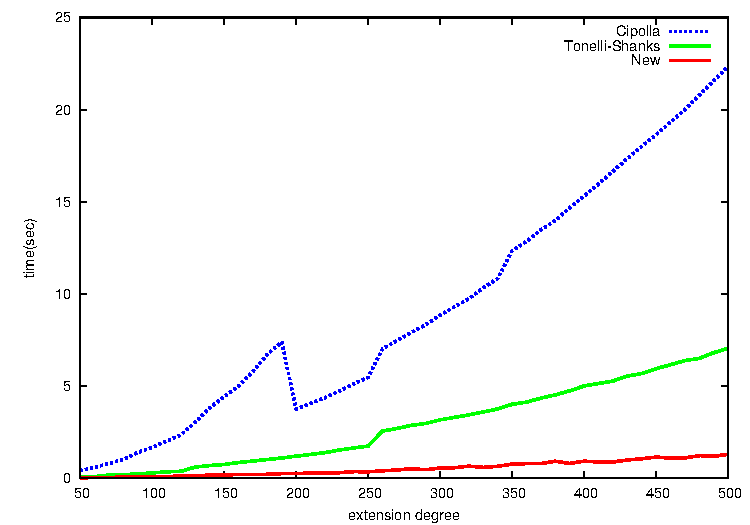
\includegraphics[width = 8cm]{sqrtTimingSP.pdf}}
\subfloat[$p = 348975609381470925634534573457497$]
{\label{figure:sqrtTimingBP}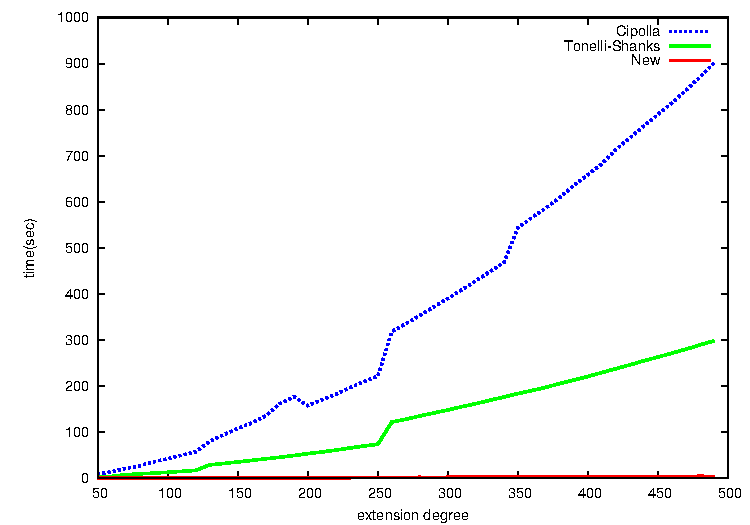
\includegraphics[width = 8cm]
{sqrtTiming.pdf}}
\end{flushleft}
\caption{\small Our square root algorithm vs. Cipolla's and
  Tonelli-Shanks' algorithms.}
\label{figure:sqrtTiming}
\end{figure}

Remember that the bottleneck in Cipolla's and Tonelli-Shanks'
algorithms is the exponentiation, which takes $O(n\MM(n)\log(p))$
operation in $\F_p$. As it turns out, NTL's implementation of modular
composition has $\omega=3$; this means that with this implementation
we have $\CC(n)=O(n^2)$, and our algorithm takes expected time
$O(\MM(n)\log(p)+n^2 \log(n))$. Although this implementation is not
subquadratic in $n$, it remains faster than Cipolla's and
Tonelli-Shanks' algorithms, in theory and in practice.

\medskip

Next, Figure~\ref{figure:sqrtTimingKvN} compares our NTL
implementation of the EDF algorithm proposed by Kaltofen and Shoup,
and our square root algorithm (note that the range of reachable
degrees is much larger that in the first figure). We ran the
algorithms for five random elements for each extension degree.  At
this scale, we observe irregularities in the averaged running time of
the Kaltofen-Shoup algorithm, due to its probabilistic behavior.

The vertical dashed lines and the green line respectively show the
running time range, and the average running time, of Kaltofen and
Shoup's algorithm. In the case of our algorithm (the red graph), the
vertical ranges are invisible because the deviation from the average
is $\approx 10^{-2}$ seconds. 



\begin{figure}[ht]
\setlength{\abovecaptionskip}{0cm}
\begin{flushleft}
\subfloat[$p = 449$]{\label{figure:sqrtTimingSPKvN}
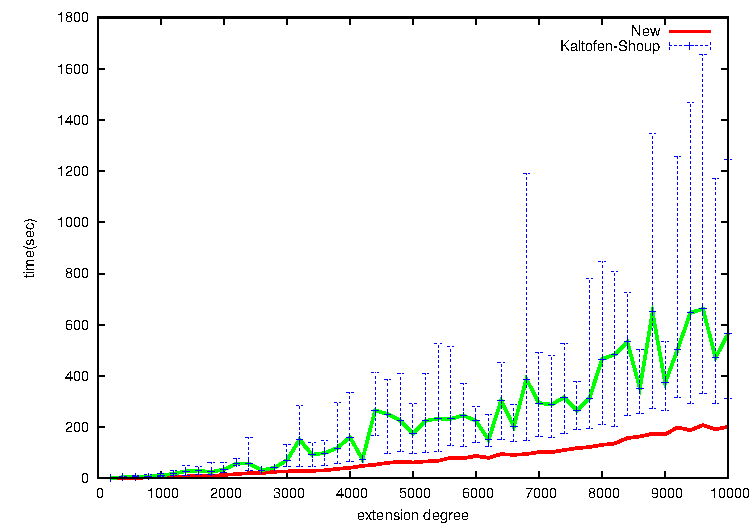
\includegraphics[width = 8cm]{sqrtTimingSPKvN.pdf}}
\subfloat[$p = 348975609381470925634534573457497$]
{\label{figure:sqrtTimingBPKvN}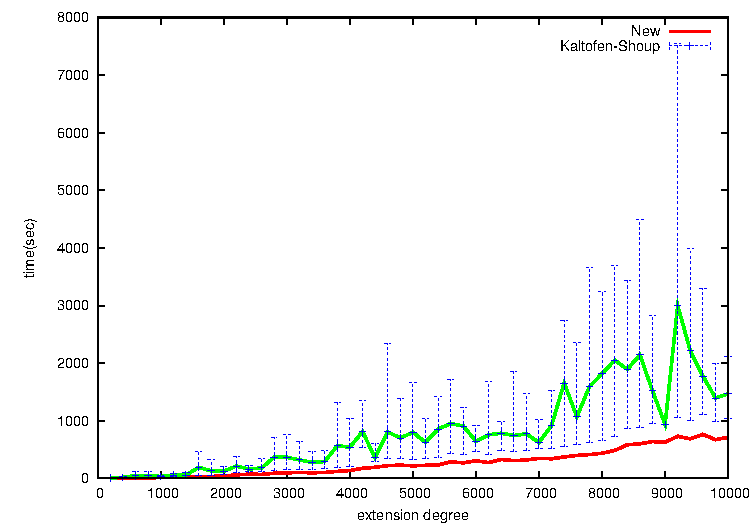
\includegraphics[width = 8cm]
{sqrtTimingKvN.pdf}}
\end{flushleft}
\caption{\small Our algorithm vs.\ Kaltofen and Shoup's algorithm.}
\label{figure:sqrtTimingKvN}
\end{figure}

This time, the results are closer.
Nevertheless, it appears that the running time of our algorithm
behaves more ``smoothly'', in the sense that random choices seem to
have less influence. This is indeed the case. The random choice in
Kaltofen and Shoup's algorithm succeeds with probability about $1/2$;
in case of failure, we have to run to whole algorithm again. In our
case, our choice of an element $c$ in $\F_q^*$ fails with probability
$1/p \ll 1/2$; then, there is still randomness involved in the $t$-th
root extraction in $\F_p$, but this step was negligible in the range
of parameters where our experiments were conducted.

Another way to express this is to compare the standard deviations in
the running times of both algorithms. In the case of Kaltofen-Shoup's
algorithm, the standard deviation is about $1/\sqrt{2}$ of the average
running time of the whole algorithm. For our algorithm, the standard
deviation is no more than $1/\sqrt{p}$ of the average running time of the
trace-like computation (which is the dominant part), plus $1/\sqrt{2}$
of the average running time of the root extraction in $\F_p$ (which is cheap).

Finally, we mention that the crossover point between our algorithm and
the previous ones varies with $p$, but is usually small: around $n=20$
to $n=30$ for small $p$ (say less than 500) and around $n=10$ to
$n=20$ for larger values of $p$. For very small degrees, the
Tonelli-Shanks algorithm was the fastest in our experiments.  Note
that for such small $n$, big-O analyses lose some significance; this
makes it difficult to get accurate theoretical estimates for the
behaviour of the various algorithms in this range of degrees.

 
\bibliographystyle{plain}
\bibliography{references}
	\graphicspath{{roots_2ext/}}

\chapter[Computing in Degree $2^k$-Extensions of Finite Fields of \\ Odd Characteristic]
{Computing in Degree $2^k$-Extensions of Finite Fields of Odd Characteristic}
\label{chapter:2ext-op}

\section{Introduction}\label{section:intro}


Factoring polynomials and constructing irreducible polynomials are two
fundamental operations for finite field arithmetic. As of now, there
exists no deterministic polynomial time algorithm for these questions
in general, but in some cases better answers can be found. In this
chapter, we discuss algorithmic questions arising in such a special case:
the construction of, and computations with, extensions of degree
$n=2^k$ of a base field, say $\F_q$, with $q$ a power of an odd prime
$p$. In other words, we are interested with the complexity of
computing in the quadratic closure of $\F_q$.

There exists a well-known construction of such
extensions~\cite[Th.\ VI.9.1]{Lang02}, which was already put to use
algorithmically in~\cite{Shoup94}: if $q=1\bmod 4$, then for any
quadratic non-residue $\alpha \in \F_q$, the polynomial
$X^{2^k}-\alpha \in \F_q[X]$ is irreducible for any $k \ge 0$, and
allows us to construct $\F_{q^{2^k}}$. If $q=3\bmod 4$, we first
construct a degree-two extension $\F_{q'}$ of $\F_q$, which will thus
satisfy $q' = 1 \bmod 4$; this is done by remarking that $X^2+1 \in
\F_q[X]$ is irreducible, so that we can construct $\F_{q'}$ as
$\F_q[X]/\langle X^2+1 \rangle$.

In this note, taking this remark as a starting point, we give fast
algorithms for operations such as multiplication and inversion, trace
and norm computation, and most importantly square root computation in
$\F_{q^{2^k}}$ (see below for our motivation), as well as isomorphism
computation. 

We do not make any assumption on the way $\F_q$ is represented: the
running time of our algorithms is estimated by counting operations
$(+,\times,\div)$ in $\F_q$ at unit cost.  The cost of most algorithms
will be expressed in terms of the cost of polynomial
multiplication. Explicitly, we let $\MM:\N\to\N$ be such that degree
$n$ polynomials over any ring $R$ can be multiplied in $\MM(n)$
operations in $R$, and such that $\MM(n)/n$ is non-decreasing (this
will be referred to as {\em super-linearity}). Using the algorithm
of~\cite{CaKa91}, we can take $\MM(n)=O(n \log(n)\log\log(n))$.

In view of the discussion above, we will assume that $q = 1 \bmod 4$:
if this is not the case, replacing $\F_q$ by $\F_{q'}$ as explained
above only induces a constant overhead, since all operations
$(+,\times,\div)$ in $\F_{q'}$ can be done using $O(1)$ operations in
$\F_q$. Besides, we will assume that the non-quadratic residue
$\alpha$ is given; otherwise, such an $\alpha$ can be found by
testing an expected $O(1)$ random elements in $\F_q$ for quadratic
residuosity. This remains a core non-deterministic component of the
construction, since finding $\alpha$ in a polynomial-time
deterministic manner is a well-known open question. Some algorithms
below are non-deterministic (Las Vegas) as well; for such algorithms,
we give the expected running time.

\begin{theorem}\label{theo:main}
  Suppose that $q=1 \bmod 4$. Given a non-quadratic residue $\alpha
  \in \F_q$, for $k \ge 0$ and $n=2^k$, the running times for
  computations in $\F_{q^n}$ reported in Table~\ref{tab1} hold.
\end{theorem}

\begin{table}[h]
\begin{center}
\begin{tabular}{c|c}
Operation & Cost \\
\hline
addition / subtraction & $O(n)$\\
multiplication & $\MM(n)+O(n)$\\
inversion & $O(\MM(n))$\\
Frobenius & $O(n+\log(q))$\\
norm & $O(\MM(n))$ \\
trace & 1 \\ 
quadratic residuosity & $O(\MM(n)+\log(q))$ \\
square root &  $O(\MM(n)\log(nq))$\ \ (expected) \\
isomorphism &  $O(n + \log(n)\log(q))$\ \ (expected)
\end{tabular}
  \caption{Costs for computations in $\F_{q^n}$, with $n=2^k$.}
  \label{tab1}
\end{center}
\end{table}

This paper can be seen as an
analogue of~\cite{DeSc12}, which discusses these questions for
Artin-Schreier extensions: the problems we consider, the techniques we
use, and the applications (dealing with torsion points of some genus 1
or 2 Jacobians; see below) are similar. More precisely, the recursive 
techniques used here are similar to those in the reference in terms of 
exploiting the special structure of the tower and the defining polynomials.

For some questions, such as Frobenius or isomorphism computation, we
refer to the next section for a precise description of the operation
we perform; however, we mention that in all cases, we use a polynomial
basis representation for all computations. In all cases, the combined
size of input and output is $O(n)$ elements in $\F_q$, and using fast
multiplication, all running times reported here are quasi-linear\footnote{
An algorithm is quasi-linear time in $n$ if it has complexity $O(n\log^kn)$
for a constant $k$.} in $n$.

Some results in the above table are straightforward (such as addition
/ subtraction or trace computation) and some are well-known (such as
multiplication). Our focus in this note is actually on square root
computation, and to the best of our knowledge, this is the first time
that such results appear. 

The straightforward approaches to square root extraction, using for
instance Cipolla's or the Tonelli-Shanks
algorithms~\cite{Tonelli1891, Cipolla1903, Shanks1972} require a number
of multiplications in $\F_{q^n}$ proportional to $\log(q^n)$; the
cost is then $O(n \MM(n)\log(q))$ operations in $\F_q$, which is
at best quadratic in $n$. It is possible to compute square roots faster,
using fast algorithms for {\em modular composition}, which is the
operation that consists in computing $F(G) \bmod H$,  given some
univariate polynomials $F,G,H$. Let us denote by $\CC(n)$ the cost of
this operation, when $F,G,H$ have all degree at most $n$. Then, the
algorithms of~\cite{KaltofenShoup1997,DlsSch2011} compute square roots
in $\F_{q^n}$ using $O(\MM(n)\log(q) + \CC(n)\log(n))$ operations in
$\F_q$.

In our model, where operations in $\F_q$ are counted at unit cost, the
best known bound on $\CC(n)$ is $\CC(n)=O(\sqrt{n}\MM(n) +
n^{(\omega+1)/2})$, where $2 \le \omega \le 3$ is such that matrices
of size $m$ over $\F_q$ can be multiplied in $O(m^\omega)$ operations \cite{BrKu78}.
Thus, depending on $\omega$, and neglecting logarithmic factors, the
cost (with respect to $n$) of the corresponding square root algorithms
ranges between $O(n^{3/2})$ and $O(n^{2})$. We remark however that, in
a boolean model (on a RAM, using an explicit boolean representation of the
elements in $\F_q$, and counting boolean operations at unit cost),
Kedlaya and Umans gave in~\cite{KeUm11} an algorithm of cost
$n^{1+\varepsilon} \log(q)^{1+o(1)}$ for modular composition in
$\F_q$, for any $\varepsilon > 0$. In that model, algorithms such as
those in~\cite{KaltofenShoup1997,DlsSch2011} are thus close to linear time.

None of the algorithms mentioned above is dedicated to the specific
case we consider, where the extension degree $n$ is a power of two;
few references consider explicitly this particular 
case~\cite{FeNoMo03, FeNoMo05}. 

The algorithm of~\cite{FeNoMo03} gives a quadratic residuosity test
that uses $O(\log(n))$ Frobenius computations and multiplications in
$\F_{q^n}$, and $O(\log(q))$ multiplications in $\F_q$. This reference
does not specify how to represent the extensions of $\F_q$, and what
algorithms should be used for basic operations.  Using the algorithms
given below for arithmetic and Frobenius computations, the cost of
their quadratic residuosity test algorithm is $O((\MM(n) +
\log(q))\log(n))$ multiplications in $\F_q$; this is slightly slower
than our result.  The authors of \cite{FeNoMo03} also give algorithms
for quadratic residuosity and square root computation for degree
$2^k$-extensions in their later work \cite{FeNoMo05}. They removed the
computation overlap between quadratic residuosity test and square
root, but the algorithms still run in times quadratic in $n$ (the
quadratic residuosity test being the bottleneck).

\medskip

This work was inspired by computations with Jacobians of curves of
genus 2 over finite fields. Given a genus 2 curve $C$ defined over
$\F_p$, the algorithm of~\cite{GaSc12} computes the cardinality of the
Jacobian $J$ of $C$, following Schoof's elliptic curve point counting
algorithm~\cite{Schoof85}. This involves in particular the computation
of successive divisors of $2^k$-torsion in $J$, by means of successive
divisions by two in $J$. Such a division by two boils down to several
arithmetic operations, and four square root extractions; thus, the
divisors we are computing are defined over the quadratic closure of
$\F_p$, or of a small extension of $\F_p$.

In other words, for dealing with $2^k$-torsion, the algorithm
of~\cite{GaSc12} relies entirely on the operations above, arithmetic
operations and square root extraction. At the time of
writing~\cite{GaSc12}, the authors relied on a variant of the
Kaltofen-Shoup algorithm~\cite{KaltofenShoup1997} with running time
$O(\MM(n)\log(q) + \CC(n)\log(n))$, which was a severe bottleneck; our
new algorithms completely alleviate this issue.

\medskip

After proving Theorem~\ref{theo:main} in Section~\ref{sec:proof}, we
present in Section~\ref{sec:exp} some experiments that confirm that
the practical interest of our quasi-linear algorithms for the
point-counting problem above.

\paragraph{Acknowledgements.} The authors are supported by NSERC and
the Canada Research Chairs program. We wish to thank the reviewers for
their helpful remarks and suggestions.

%%%%%%%%%%%%%%%%%%%%%%%%%%%%%%%%%%%%%%%%%%%%%%%%%%
%%%%%%%%%%%%%%%%%%%%%%%%%%%%%%%%%%%%%%%%%%%%%%%%%%

\section{Proof of the complexity statements}\label{sec:proof}

In this section, we prove the results stated in Table~\ref{tab1}.
The tower of fields $\F_q,\F_{q^2},\dots\F_{q^{2^k}},\dots$ will be
written
$$\L_0 \subset \L_1 \subset \cdots \subset \L_k \subset \cdots,$$ with
$\L_k = \F_{q^{2^k}}$ for all $k$.

%=================================================

\subsection{Representing the fields $\L_k$}

The tower of fields $\L_0,\L_1,\dots$ can be represented in two
fashions, using univariate or multivariate representations (see as
well~\cite{DeSc12}, for a similar discussion for Artin-Schreier
extensions).

Let $\alpha\in\F_q$ be a fixed non-quadratic residue.  Define the
sequence of polynomials $T_1,T_2,\dots$ in indeterminates
$X_1,X_2,\dots$ given by
$$T_1 = X_1^2-\alpha \quad\text{and}\quad T_k = X_k^2-X_{k-1}
\quad\text{for $k > 1$},$$ as well as the polynomials $P_1,P_2,\dots$ given by
$$P_k = X_k^{2^k} - \alpha\quad\text{for $k \ge 1$}.$$The discussion
in the introduction, as well as the one in~\cite{Lang02}, shows that for 
all $k \ge 0$ we have the equality between ideals
\begin{equation}\label{eq:TP}
\langle T_1,\dots,T_k \rangle = \langle P_k, X_{k-1}-X_k^2, \dots,
X_1-X_k^{2^{k-1}} \rangle,
\end{equation}
that this ideal (call it $A_k$) is prime, and that we have
$$\L_k \simeq \F_q[X_1,\dots,X_k]/ A_k.$$ 
For $k \ge 1$, let $x_k$ be the image of $X_k$ in the residue class
ring $\F_q[X_1,\dots,X_k]/A_k$.  Due to the natural embedding of
$\F_q[X_1,\dots,X_k]/ A_k$ into $\F_q[X_1,\dots,X_{k+1}]/ A_{k+1}$,
$x_k$ can be unequivocally seen as an element of $\F_{q^{2^\ell}}$ for $\ell
\ge k$ (and thus as an element of the quadratic closure of $\F_q$).

On the left-hand side of~\eqref{eq:TP}, we have a Gr{\"o}bner basis of
$A_k$ for the lexicographic order $X_1 < \cdots < X_k$, whereas on the
right we have a Gr{\"o}bner basis for the lexicographic order $X_k <
\cdots < X_1$. Corresponding to these two bases of $A_k$, the elements
of $\L_k$ can be represented as polynomials in $x_1,\dots,x_k$ of
degree at most $1$ in each variable (and coefficients in $\F_q$), or
as polynomials in $x_k$ of degree less than $2^k$.

By default, we will use the univariate representation; an element
$\gamma$ of $\L_k$ will thus be written as $\gamma=G(x_k)$, for some
polynomial $G \in \F_q[X_k]$ of degree less than $2^k$.

We will not explicitly need to convert to multivariate polynomials,
but we will often do one step of such a conversion, switching between
univariate and bivariate bases. Indeed, for all $k \ge 1$, we have
$$\L_k \simeq \F_q[X_k]/\langle P_k(X_k) \rangle \simeq \F_q[X_{k-1},X_k]/\langle
P_{k-1}(X_{k-1}), X_k^2-X_{k-1}\rangle.$$ The $\F_q$-monomial basis of
$\F_{q^{2^k}}$ associated to the left-hand side is
$$1,\ x_k,\ \dots,\ x_k^{2^k-1},$$ whereas the one associated to the
right-hand side is
$$1,\ x_{k-1},\ \dots,\ x_{k-1}^{2^{k-1}-1},\ x_k,\ x_{k-1}x_k,\ \dots,\ x_{k-1}^{2^{k-1}-1}x_k.$$
The change-of-basis from the univariate basis to the bivariate one
amounts to writing an expression $G(x_k)$, with $G$ of degree less
than $2^{k}$, as
$$G(x_k) = G_0(x_k^2) + x_k G_1(x_k^2) = G_0(x_{k-1}) + x_k
G_1(x_{k-1}),$$ with $G_0$ and $G_1$ of degrees less than
$2^{k-1}$. This does not require any arithmetic operation; the same
holds for the converse change-of-basis. Continuing this way on $G_0$
and $G_1$, we could convert between univariate and multivariate bases
without arithmetic operations if needed.

%=================================================

\subsection{Arithmetic operations}

In this subsection, we discuss the cost of arithmetic operations
$(+,\times,\div)$ in $\L_k$, for some $k \ge 0$.  In all that follows,
we write $n=[\L_k:\F_q]$, that is, $n=2^k$.

Addition and subtraction take time $O(n)$. For multiplication, using
the univariate basis leads to a cost of $\MM(n)+O(n)$ operations in
$\F_q$, where the $O(n)$ term accounts for reduction modulo $P_k$
(this takes linear time, since $P_k$ is a binomial). Note that a
non-trivial (and slightly less efficient) approach using the
multivariate representation is in~\cite{BoChHoSc11}.

For inversion, in the univariate basis, a natural idea is to use the
fast extended GCD algorithm for univariate
polynomials~\cite[Ch.~11]{GaGe03}, resulting in a running time
$O(\MM(n)\log(n))$. However, better can be done by using the tower
structure of the fields $\L_k$.  Indeed, consider $\gamma=G(x_k) \in
\L_k^\times$. Then, writing $G(x_k) = G_0(x_{k-1}) + x_k
G_1(x_{k-1}),$ we have
\begin{align*}
\frac{1}{G(x_k)}
&= \frac{1}{G_0(x_{k - 1}) + x_kG_1(x_{k - 1})}\\ 
&= \frac{G_0(x_{k-1}) - x_kG_1(x_{k-1})}{G_0(x_{k - 1})^2 - x_{k - 1}G_1(x_{k - 1})^2}.
\end{align*}
Therefore, computing an inverse in $\L_k$ amounts to $O(1)$ additions
and multiplications in $\L_k$, and one inversion in $\L_{k-1}$. This
gives a recursive algorithm with cost $T(k) = T(k-1) + O(\MM(2^k))$;
the super-linearity of $\MM$ implies that the running time is
$O(\MM(2^k))=O(\MM(n))$ operations in $\F_q$.

%=================================================

\subsection{Frobenius computation}

Let $\gamma$ be in $\L_k$, and let $r = q^d$ for some positive integer
$d$. We explain here how to compute $\gamma^r \in \L_k$; as above,
we write $n=2^k$.

We start with the case $\gamma=x_k$: writing $r = n u + v$ with $0 \le
v < n$, and using the fact that $x_k^n=\alpha$, we obtain $x_k^r =
\alpha^u x_k^v$. The constant $\alpha^u = \alpha^{u \bmod (q-1)}$ can
be computed in $O(\log(q))$ multiplications in $\F_q$ by repeated
squaring.  Although our focus is on counting $\F_q$-operations, we
also mention how to compute $u \bmod (q-1)$ and $v$ efficiently: first
of all, we compute $\rho=r\bmod n(q-1)$ by repeated squaring; then, $u
\bmod (q-1)$ and $v$ are respectively the quotient and remainder in
the division of $\rho$ by $n$. They can be computed with a boolean
cost polynomial (and actually, quasi-linear) in $\log(d)\log(nq)$,
since the bottleneck is an exponentation with exponent $O(d \log(q))$,
modulo an integer of bit size $O(\log(nq))$.

For a general $\gamma$ of the form $\gamma=G(x_k)$, 
writing $G(x_k) = g_{n - 1}x_k^{n - 1} + \cdots + g_1x_k + g_0$, we have
\begin{align*}
\gamma^r 
&= g_{n - 1}(x_k^r)^{n - 1} + \cdots + g_1(x_k^r) + g_0 \\
&= g_{n - 1}(\alpha^u x_k^v)^{n - 1} + \cdots + g_1(\alpha^u x_k^v) + g_0.
\end{align*}
Knowing $\alpha^u$ and $v$, computing $\gamma^r$ amounts to compute
the first $n$ powers of $\alpha^u x_k^v$ and substituting them in
$G$. Since $x_k^{n}=\alpha$, these powers are all monomials in $x_k$,
and can be computed successively in $O(n)$ multiplications in
$\F_q$. Therefore, computing the Frobenius takes a total of
$O(n+\log(q))$ operations in $\F_q$.

%=================================================

\subsection{Trace, norm and quadratic residuosity test}

The norm $\norm_{\L_k/\F_q}$ and the trace $\trace_{\L_k/\F_q}$
are easy to compute, using transitivity. Indeed, for $\gamma \in
\L_k$, we have
$$\norm_{\L_k / \F_q}(\gamma) = \norm_{\L_1 / \F_q}(\norm_{\L_2 / \L_1}(\cdots \norm_{\L_k / \L_{k -
    1}}(\gamma)))$$
and
$$\trace_{\L_k / \F_q}(\gamma) = \trace_{\L_1 / \F_q}(\trace_{\L_2 /
  \L_1}(\cdots \trace_{\L_k / \L_{k - 1}}(\gamma))).$$ Write as before
$\gamma=G(x_k)$ and $G=G_0(x_{k-1})+x_k G_1(x_{k-1})$.  Then, we have
$$\norm_{\L_k / \L_{k - 1}}(\gamma) =  G_0(x_{k - 1})^2 - x_{k - 1}G_1(x_{k - 1})^2$$
and
$$\trace_{\L_k / \L_{k - 1}}(\gamma) = 2G_0(x_{k - 1}),$$ since in the
quadratic extension $\L_k$ of $\L_{k-1}$ generated by $x_k^2-x_{k-1}$,
the norm (resp.\ trace) of $\gamma$ is the product (resp.\ sum) of
$\gamma$ and its conjugate $\gamma'=G_0(x_{k-1})-x_k G_1(x_{k-1})$.

To compute the norm of $\gamma$, this gives a recursive algorithm
using one recursive call and $O(1)$ multiplications in each extension;
using the super-linearity of $\MM$ (as for inversion), the total is
$O(\MM(n))$ operations in $\F_q$. For the trace, by transitivity, we
obtain $\trace_{\L_k / \F_q}(\gamma) = n g_0$ where $g_0$ is the constant
term of $G$; this could also have been deduced from the fact that the
trace of $\gamma=G(x_k)$ in the extension $\L_k=\F_q[X_k]/\langle P_k
\rangle$ is the coefficient of $X_k^{n-1}$ in $G P'_k \bmod P_k$.  At
any rate, the trace is computed using $1$ multiplication in $\F_q$

Finally, to check if $\gamma$ is a quadratic residue we compute
$\gamma^{(q^n - 1) / 2} = \norm_{\L_k / \F_q}(\gamma)^{(q - 1) / 2}$; this
takes $O(\MM(n) + \log(q))$ operations in $\F_q$ (using repeated squaring
for the exponentiation).

Let us briefly comment on alternative derivations of the norm and the
trace; they are slightly less efficient, but these ideas will allow us
to compute square roots in the next subsection (the underlying idea is
not new; it appears for instance in~\cite{GaSh92,FeNoMo03}).
Fix $n$ and $\gamma$ as above and for $m \ge 0$, define
$$N_m(\gamma) = \gamma^{1 + q + q^2 + \cdots + q^{m - 1}}$$ to be the
{\em $m$-norm} of $\gamma$. Similarly, the {\em $m$-trace} of $\gamma$
is defined to be $T_m(\gamma) = \gamma + \gamma^q + \cdots +
\gamma^{q^{m - 1}}$ (this is called a pseudo-trace
in~\cite{DeSc12}). For $m=n$, we recover the standard norm and trace.

Writing
$$\zeta_m = \gamma^{q + q^2 + \cdots + q^m},$$ we have $N_m(\gamma) = \gamma\zeta_{m
  - 1}$. The element $\zeta_m$ can be computed efficiently by means
of the formulas
\begin{equation}
\label{eq:zeta}
\zeta_1 = \gamma^q \quad\text{and}\quad
\zeta_m = 
\begin{cases}
\zeta_{m / 2}\zeta_{m / 2}^{q^{m / 2}} & \text{if $m$ is even}  \\
\zeta_1\zeta_{m - 1}^{q} & \text{if $m$ is odd.}
\end{cases} 
\end{equation}
(We could compute $N_m(\gamma)$ directly using a similar recurrence,
but we will reuse the $\zeta_m$ in the next subsection.)  Computing
$\zeta_1$ is done by means of one Frobenius computation.  Deducing
$\zeta_m$ from either $\zeta_{m / 2}$ or $\zeta_{(m-1) / 2}$ takes
$O(1)$ Frobenius and multiplications. Thus, the total for $\zeta_m$,
and thus $N_m(\gamma)$, is $O(\log(m))$ Frobenius and multiplications
in $\L_k$, which amounts to $O(\MM(n)\log(m)+\log(q)\log(m))$
operations in $\F_q$.

If needed, the $m$-trace can be computed similarly to the $m$-norm by
the following recursion:
$$T_1 = \gamma \quad\text{and}\quad
T_m = 
\begin{cases}
T_{m / 2} + T_{m / 2}^{q^{m / 2}} & \text{if $m$ is even}  \\
T_1 + T_{m - 1}^{q} & \text{if $m$ is odd.}
\end{cases}
$$ Therefore, $T_m(\gamma)$ can be computed using $O(\log(m))$
Frobenius and additions, hence the overall running time
$O(n\log(m)+\log(q)\log(m))$.


%=================================================

\subsection{Taking square roots}\label{section:sqrt}

In this subsection, we review the idea presented in \cite{DlsSch2011}
to compute square roots, and adapt it to our situation, where
computing a Frobenius is cheap.


Let $\delta \in \L_k^\times$ be given, assume that $\delta$ is a
square and let $\gamma \in \L_k$ be an (unknown) square root of
it. Define $\beta \in \F_q$ as the (unknown) quantity
\begin{equation}
\label{equation:tr-square}
\begin{aligned}
\beta = \trace_{\L_k / \F_q}(\gamma) = \sum_{i = 0}^{n - 1} \gamma^{q^i}
& = \gamma(1 + \gamma^{q - 1} + \gamma^{q^2 - 1} + \cdots + \gamma^{q^{n - 1} -1}) \\
& = \gamma(1 + \delta^{(q - 1) / 2} + \delta^{(q^2 - 1) / 2} + \cdots + \delta^{(q^{n - 1} -1) / 2})\\
& = \gamma \eta,
\end{aligned}
\end{equation}
with
$$\eta = 1 + \delta^{(q - 1) / 2} + \delta^{(q^2 - 1) / 2} + \cdots +
\delta^{(q^{n - 1} -1) / 2}.$$ We may assume $\eta \ne 0$; otherwise,
we can replace $\delta$ by $\delta' = \delta c^2$ for a random element
$c \in \L_k^\times$. We expect to have $\trace_{\F_q / \F_{q'}}(\gamma c) \ne 0$ 
after $O(1)$ trials: There are $q^{2^k} / q$ values of $c$ for which the trace is zero, 
and hence the probability of having a non-zero trace is $1 - (q^{2^k} / q) / q^{2^k} = 1 - 1/q
\ge 1/2$. Squaring both sides of Eq.~\eqref{equation:tr-square}
results in the quadratic equation $\beta^2 = \delta \eta^2$ over
$\F_q$.

Provided $\eta$ is known, $\beta$ can be deduced from this quadratic
equation, and finally $\gamma$ as $\gamma=\beta \eta^{-1}$.  Computing
$\beta$ from the above quadratic equation takes an expected
$O(\log(q))$ operations in $\F_q$~\cite[Ch.\ 14.5]{GaGe03}, so that
computing $\eta$ is the key to computing $\gamma$ efficiently. This
can be done as follows.

Let $\lambda \in \L_k$ be defined by $\lambda = \delta^{(q - 1) /
  2}$; then, $\eta$ is given by
$$
\eta = 1 + \lambda + \lambda^{1 + q} + \lambda^{1 + q + q^2} + \cdots + \lambda^{1 + q + q^2 + \cdots + q^{n-2}}.
$$
For $m \ge 0$, define 
$$\varepsilon_m = \lambda^{q} + \lambda^{q + q^2} + \cdots +
\lambda^{q + q^2 + \cdots + q^m},$$ so that $\eta= 1 + \lambda+
\lambda \varepsilon_{n-2}$, and recall as well the definition of
$\zeta_m = \lambda^{q + q^2 + \cdots + q^m}.$ Then, similar to the
recurrence relation given in~\eqref{eq:zeta} for $\zeta$, the following
holds for $\varepsilon$:
\begin{equation}\label{eq:varepsilon}
\varepsilon_1 =
\lambda^q \quad\text{and}\quad 
\varepsilon_m = 
\begin{cases}
\varepsilon_{m / 2} + \zeta_{m / 2}\varepsilon_{m / 2}^{q^{m / 2}} & \text{if $m$ is even}  \\
\varepsilon_{m-1} + \zeta_m & \text{if $m$ is odd}
\end{cases}  
\end{equation}
Computing $\lambda$ takes $O(\MM(n)\log(q))$ operations in $\F_q$;
then, we obtain the initial values $\zeta_1$ and $\varepsilon_1$ using
$O(1)$ Frobenius. Assume, inductively, that we have computed
$\varepsilon_m$, $\zeta_m$. Then, using Eqs.~\eqref{eq:zeta}
and~\eqref{eq:varepsilon}, $\zeta_{2m}$ and $\varepsilon_{2m}$, or
$\zeta_{2m+1}$ and $\varepsilon_{2m+1}$, can be computed using $O(1)$
Frobenius and $O(1)$ multiplications in $\F_{q^n}$. Therefore,
$\varepsilon_n$, and altogether $\eta =
1+\lambda+\lambda\varepsilon_{n-2}$ can be computed using
$O(\MM(n)\log(q)+\MM(n)\log(n))=O(\MM(n)\log(nq))$ operations in $\F_q$.
We have seen that deducing $\beta$ takes an expected $O(\log(q))$
operations in $\F_q$, and the cost of computing $\gamma$ is negligible
compared to the computation of $\eta$. Thus, the overall running time
is an expected $O(\MM(n)\log(nq))$ operations in $\F_q$.

%=================================================

\subsection{Computing embeddings}

We finally consider the problem of computing embeddings and
isomorphisms between two different ``towers'' defining the quadratic
closure of $\F_q$.  Consider $\L_k = \F_q[X_k]/\langle P_k \rangle$
and $\L'_j = \F_q[Y_j]/\langle Q_j\rangle$,  $k, j$ positive
integers, where we write
$$P_k = X_k^{2^k} - \alpha\quad\text{and}\quad Q_j = Y_j^{2^j} -
\beta,$$ for some non-quadratic residues $\alpha,\beta$ in $\F_q$.
Assuming for instance that $k \le j$, $\L_k$ can be identified as a
subfield of $\L'_j$; we show how to compute an embedding $\phi : \L_k
\hookrightarrow \L'_j$ efficiently. As before, we denote by $x_k$ the
image of $X_k$ in $\L_k$, and by $y_j$ the image of $Y_j$ in $\L'_j$;
we write $n=2^k$ and $m=2^j$.

The idea is straightforward: we first find a root $\rho$ of $P_k$ in
$\L'_j$; then, the mapping $\phi: \L_k \to \L'_j$ given by
$\phi(G(x_k)) = G(\rho) \bmod Q_j$ is well-defined and gives an
isomorphism of $\L_k$ onto its image. To find the root $\rho$ of
$P_k$ in $\L'_j$, one has to take $k$ successive square roots of
$\alpha$ in $\L'_j$. For this, we could use the algorithm of the
previous subsection, but since we start from $\alpha \in \F_q$, better
can be done.

Let us look at a slightly more general question: given $\mu \in \F_q$
and an even integer $\ell \ge 0$, compute a square root of $\mu
y_j^\ell$:
\begin{itemize}
\item if $\mu$ is a square in $\F_q$, say $\mu=\nu^2$, $\nu
  y_j^{\ell/2}$ is a square root of $\mu y_j^\ell$;
\item else, $\mu/\beta$ is a square in $\F_q$, say $\mu/\beta =
  \nu^2$; then $\nu y_j^{2^{j-1}+\ell/2}$ is a square root
  of $\mu y_j^\ell$.
\end{itemize}
Since we start with $\ell=0$, we can repeat the process at least $j$
times, and thus in particular at least $k$ times; the cost is thus
that of $O(k)=O(\log(n))$ quadratic residuosity tests, square-root
computations and arithmetic operations in $\F_q$; this uses an
expected $O(\log(q)\log(n))$ operations in $\F_q$.
Since the root $\rho$ we obtain is of the form $\rho=\mu
y_j^\ell$ for some $\ell < m$, computing $G(\rho) \mod Q_j$, for some
$G$ of degree less than $n$ (and thus than $m$), takes $O(m)$
multiplications in $\F_q$ (as was the case for Frobenius computation).

For isomorphism computation, taking $k=j$, and thus $m=n$, gives
the claimed bound $O(n + \log(q)\log(n))$ operations in $\F_q$.

%%%%%%%%%%%%%%%%%%%%%%%%%%%%%%%%%%%%%%%%%%%%%%%%%%
%%%%%%%%%%%%%%%%%%%%%%%%%%%%%%%%%%%%%%%%%%%%%%%%%%

\section{Experiments}\label{sec:exp}

We conclude this section with experiments using an implementation of
our algorithms based on NTL~\cite{NTL2009}. All running times are
obtained on an Intel Xeon CPU. In all cases, we start from the base
field $\F_p$.

First, we consider square root computation. For computing square roots
in an extension $\F_{p^n}$, without assumption on $n$, we used
in~\cite{DlsSch2011} modular polynomial composition, resulting in the
running time $O(\MM(n)\log(p) + \CC(n)\log(n))$. In cases where $n$ is
a power of two, the results in this paper are superior in terms of
complexity; Figure~\ref{figure:sqrtTiming} confirms that this is also
the case in practice. In that figure, we take the ``random'' prime $p
= \seqsplit{348975609381470925634534573457497}$ already used
in~\cite{DlsSch2011}, and different values of the extension degree~$n$,
that are always powers of two; see below for the reasons behind our
choice of such a large value of $p$.

\begin{figure}[ht]
\begin{center}
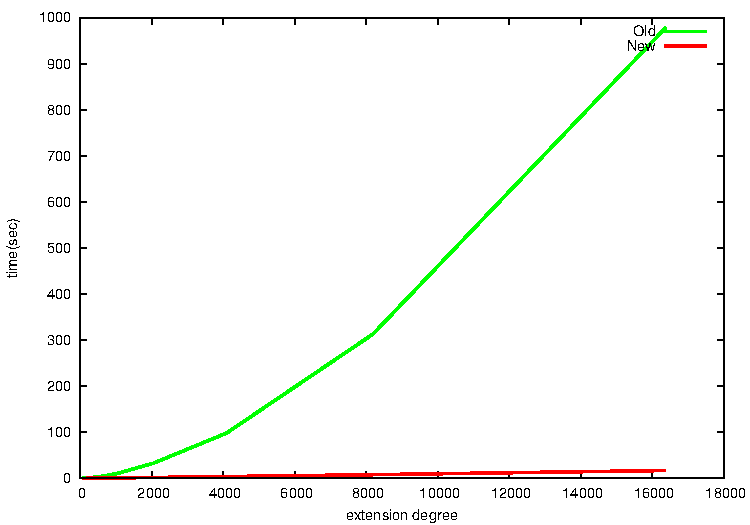
\includegraphics[width = 9cm]{sqrtTiming.pdf}
\end{center}
\caption{\small The new square root algorithm vs. the one in \cite{DlsSch2011}}
\label{figure:sqrtTiming}
\end{figure}

Table~\ref{table:2-tor-timings} gives timings (in seconds) for the
genus 2 point-counting application described in the introduction.  The
table describes the various ingredients involved in computing
successive $2^k$-torsion divisors in the Jacobian of the (randomly
chosen) curve $C$:
\[
\begin{array}{rcl}
y^2 &=& 
x^5 + 67412365472663169119085380769732137727\, x^4 \\
&& + 132706051439871719391705031627238584248\, x^3 \\
&& + 150906984006321211274278480789580538770\, x^2 \\
&& + 5602222826077482782805347307759926224\, x \\
&& + 157456212652423046465778673243920804193.
\end{array}
\]
over $\vmathbb{F}_p$ with $p = 2^{127} - 1$ (this 127 bit prime is the
one used in the records described in~\cite{GaSc12}). Once these
divisors are known, they are used to compute the cardinality of the
Jacobian $J$ of $C$ modulo $2^k$ (more exactly, we compute the image
modulo $2^k$ of the characteristic polynomial of the Frobenius
endomorphism on $J$); this last step is not detailed here, we will
refer to it as the {\em search} step.

In Table~\ref{table:2-tor-timings}, the degree $e_k$ is the degree of
the field extension over which the successive divisors are
defined. There are two main rows: the first one gives the timings for
computing all required square roots (which give us the required
$2^k$-torsion divisors); the second row gives the timing for the
search step, which involves arithmetic operations in the current
extension of $\F_p$. For a more precise profiling, each of the two
main rows is divided into three subrows labelled with \Romnum{1},
\Romnum{2}, and \Romnum{3}: \Romnum{1} denotes the original Gaudry and
Schost implementation~\cite{GaSc12}; \Romnum{2} and \Romnum{3} denote
the same implementation but using the algorithm in \cite{DlsSch2011}
and the one in Section \ref{section:sqrt} respectively. All square root
algorithms in this table are probabilistic.

In previous implementations, square root computation was a clear
bottleneck; with our new algorithm, it has now become a minor
component of the running time.



\begin{center}
\renewcommand{\multirowsetup}{\centering}
\renewcommand{\tabcolsep}{1.7mm}
% preventing the expont to touch the top of the cell
\newlength{\lengthofcell}
\newcommand{\pboxc}[1]{
\settowidth{\lengthofcell}{#1}
\parbox{\lengthofcell}{#1}}
%------------------------------------
\begin{table}[ht]
\centering
\begin{tabular}{c|c||c|c|c|c|c|c|c|c|c|c|c|c}
\multicolumn{2}{c||}{index $2^k$} & \pboxc{$2^{6}$} & \pboxc{$2^{7}$} & \pboxc{$2^{8}$} & \pboxc{$2^{9}$} & \pboxc{$2^{10}$} & \pboxc{$2^{11}$} & \pboxc{$2^{12}$} & \pboxc{$2^{13}$} & \pboxc{$2^{14}$} & \pboxc{$2^{15}$} & \pboxc{$2^{16}$} & \pboxc{$2^{17}$} \\
\hline\hline
\multicolumn{2}{c||}{degree $e_k$} & \pboxc{$2^{5}$} & \pboxc{$2^{6}$} & \pboxc{$2^{7}$} & \pboxc{$2^{8}$} & \pboxc{$2^{9}$} & \pboxc{$2^{10}$} & \pboxc{$2^{11}$} & \pboxc{$2^{12}$} & \pboxc{$2^{13}$} & \pboxc{$2^{14}$} & \pboxc{$2^{15}$} & \pboxc{$2^{16}$}\\
\hline\hline
\multirow{3}{2cm}{square roots} & \Romnum{1} & 0.2 & 0.4 & 1.2 & 3.5 & 11 & 33 & 109 & 365 & 1262 & 4466 & 16246 & 60689 \\  
& \Romnum{2} & 0.2 & 0.5 & 1.2 & 2.9 & 8 & 23 & 73 & 232 & 734 & 2309 & 7368 & 23604 \\ 
& \Romnum{3} & 0.1 & 0.2 & 0.5 & 1.1 & 2 & 5 & 11 & 25 & 53 & 114 & 246 & 523 \\
\hline\hline
\multirow{3}{2cm}{search step} & \Romnum{1} & 0.5 & 1.1 & 2.8 & 6.5 & 14 & 32 & 73 & 164 & 368 & 816 & 2020 & 4827  \\
& \Romnum{2} & 0.4 & 1.0 & 2.3 & 5.4 & 12 & 27 & 62 & 139 & 309 & 657 & 1609 & 3740  \\
& \Romnum{3} & 0.4 & 0.9 & 2.0 & 4.5 & 11 & 24 & 53 & 119 & 267 & 598 & 1402 & 3297 \\
\end{tabular}
\caption{Timings for lifting $2^k$-torsion}
\label{table:2-tor-timings}
\end{table}
\end{center}


\bibliographystyle{plain}
\bibliography{references}

	\graphicspath{{towers/}}

\chapter{Fast Algorithms for $\ell$-adic Towers over Finite Fields}
\label{chapter:ell-adic}

\section{Introduction}
\label{sec:intro}

Building arbitrary finite extensions of finite fields is a fundamental
task in any computer algebra system. For this, an especially powerful
system is the ``compatibly embedded finite fields'' implemented in
Magma~\cite{MAGMA,bosma+cannon+steel97}, capable of building
extensions of any finite field and keeping track of the embeddings
between the fields.

The system described in~\cite{bosma+cannon+steel97} uses linear
algebra to describe the embeddings of finite fields. From a complexity
point of view, this is far from optimal: one may hope to compute and
apply the morphisms in quasi-linear time in the degree of the
extension, but this is usually out of reach of linear algebra
techniques. Even worse, the quadratic memory requirements make the
system unsuitable for embeddings of large degree extensions. Although
the Magma core has evolved since the publication of the paper,
experiments in Section~\ref{sec:impl} show that embeddings of large
extension fields are still out of reach.

In this paper, we discuss an approach based on polynomial arithmetic,
rather than linear algebra, with much better performance. We consider
here one aspect of the question, $\ell$-adic towers; we expect that
this will play an important role towards a complete solution.

Let $q$ be a power of a prime $p$, let $\F_q$ be the finite field with
$q$ elements and let $\ell$ be a prime. Our main interest in this
paper is on the algorithmic aspects of the \emph{$\ell$-adic closure}
of $\F_q$, which is defined as follows. Fix arbitrary embeddings
\begin{equation*}
  \F_q \subset \F_{q^\ell} \subset \F_{q^{\ell^2}} \subset \cdots;
\end{equation*}
then, the $\ell$-adic closure of $\F_q$ is the infinite field defined as
\begin{equation*}
  \F_q^{(\ell)} = \bigcup_{i\ge 0}\F_{q^{\ell^i}}.
\end{equation*}
We also call an \emph{$\ell$-adic tower} the sequence of extensions
$\F_q,\F_{q^\ell},\dots$ In particular, they allow us to build the
algebraic closure $\bar{\F}_q$ of $\F_q$, as there is an isomorphism
\begin{equation}
  \label{eq:tensor}
  \bar{\F}_q \cong \bigotimes_{\ell\text{ prime}} \F_q^{(\ell)},
\end{equation}
where the tensor products are over $\F_q$; we will briefly mention
below the algorithmic counterpart of this equality.

We present here algorithms that allow us to ``compute'' in the
first levels of $\ell$-adic towers (in a sense defined hereafter); at
level $i$, our goal is to be able to perform all basic operations in
quasi-linear time in the extension degree $\ell^i$.  We do not discuss
the representation of the base field $\F_q$, and we count 
operations $\{+,-,\times,\div\}$ in $\F_q$ at unit cost.

%% Since our focus is on the representation of extensions of large
%% degree, we do not consider issues related to special representations
%% of small finite fields, such as primitive polynomials, Zech
%% logarithms, Conway polynomials, etc.

Our techniques are inspired by those
in~\cite{cantor89,couveignes00,df+schost12}, which dealt with the
Artin-Schreier case $\ell=p$ (see also~\cite{DoSc12}, which reused
these ideas in the case $\ell=2$): we construct families of
irreducible polynomials with special properties, then give algorithms
that exploit the special form of those polynomials to apply the
embeddings. Because they are treated in the
references~\cite{df+schost12,DoSc12}, {\em we exclude the cases
  $\ell=p$ and $\ell=2$}.

The field $\F_{q^{\ell^i}}$ will be represented as $\F_q[X_i]/\langle
Q_i\rangle$, for some irreducible polynomial $Q_i \in
\F_q[X_i]$. Letting $x_i$ be the residue class of $X_i$ modulo $Q_i$
endows $\F_{q^{\ell^i}}$ with the monomial basis
\begin{equation}
  \label{eq:uni-basis1}
  \uu_i = (1,x_{i},x_{i}^2,\ldots,x_{i}^{\ell^{i}-1}).
\end{equation}
Let $\MM : \N \rightarrow
\N$ be such that polynomials in $\F_q[X]$ of degree less than $n$ can
be multiplied in $\MM(n)$ operations in $\F_q$, under the
assumptions of~\cite[Ch.~8.3]{vzGG}; using FFT multiplication, one can
take $\MM(n)\in O(n\log (n) \log\log (n))$. Then, multiplications and
inversions in $\F_q[X_i]/\langle Q_i \rangle$ can be done in
respectively $O(\MM(\ell^i))$ and $O(\MM(\ell^i)\log(\ell^i))$
operations in $\F_q$~\cite[Ch.~9-11]{vzGG}. This is almost optimal, as
both results are quasi-linear in $[\F_{q^{\ell^i}}:\F_q]=\ell^i$.

Computing embeddings requires more work. For this problem, it is
enough consider a pair of consecutive levels in the tower, as any
other embedding can be done by applying repeatedly this elementary
operation. Following again~\cite{df+schost12}, we introduce two
slightly more general operations, {\em lift} and {\em push}.

To motivate them, remark that for $i \ge 2$, $\F_{q^{\ell^{i}}}$ has
two natural bases as a vector space over $\F_q$. The first one is via
the monomial basis $\uu_{i}$ seen above, corresponding to the
univariate model $\F_q[X_{i}]/ \langle Q_{i} \rangle$. The second one
amounts to seeing $\F_{q^{\ell^{i}}}$ as a degree $\ell$ extension of
$\F_{q^{\ell^{i-1}}}$, that is, as
\begin{equation}\label{eq:QiTi}
\F_q[X_{i-1},X_i]/\langle Q_{i-1}(X_{i-1}), T_i(X_{i-1},X_i)\rangle,  
\end{equation}
for some polynomial $T_i$ monic of degree $\ell$ in $X_{i}$, and of
degree less than $\ell^{i-1}$ in $X_{i-1}$.  The corresponding basis is
bivariate and involves $x_{i-1}$ and $x_i$:
\begin{equation}
  \label{eq:bi-basis}
  \bb_{i} = (1,\ldots,x_{i-1}^{\ell^{i-1}-1},\ldots,x_i^{\ell-1},\ldots,x_{i-1}^{\ell^{i-1}-1}x_i^{\ell-1}).
\end{equation}
{\em Lifting} corresponds to the change of basis from $\bb_i$ to
$\uu_i$; {\em pushing} is the inverse transformation.

Lift and push allow us to perform embeddings as a particular case, but
they are also the key to many further operations. We do not give
details here, but we refer the reader
to~\cite{df+schost12,DoSc12,LeSc12} for examples such as the
computation of relative traces, norms or characteristic polynomials,
and applications to solving Artin-Schreier or quadratic equations,
given in~\cite{df+schost12} and~\cite{DoSc12} for respectively
$\ell=p$ and $\ell=2$.

Table~\ref{table:main} summarizes our main results.  Under various
assumptions, it gives costs (counted in terms of operations in $\F_q$)
for initializing the construction, building the polynomials $Q_i$ and
$T_i$ from~Eq.\eqref{eq:QiTi}, and performing lift and push. $O_e(\ )$
indicates probabilistic algorithms with expected running time, and
$O\tilde{_e}(\ )$ indicates the additional omission of logarithmic
factors.  Two entries mention bit complexity, as they use an elliptic
curve point counting algorithm.


\begin{table}
	\resizebox{\textwidth}{!}{$
	\def\arraystretch{1.2}
	\begin{array}{c|cccc}
	\text{Condition} & \text{Initialization} & Q_i, T_i & \text{Lift, push}\\
	\hline \hline
	q = 1 \bmod \ell & O_e(\log(q))  & O(\ell^i) & O(\ell^i) \\
	q = -1 \bmod \ell & O_e(\log(q)) & O(\ell^i) & O(\MM(\ell^i) \log(\ell^i)) \\
	- & O_e (\ell^2+\MM(\ell) \log(q)) & O(\MM(\ell^{i+1})\MM(\ell)\log(\ell^i)^2) & O( \MM(\ell^{i+1})\MM(\ell)\log(\ell^i))\\
	4\ell \le q^{\sfrac{1}{4}} & O\tilde{_e}(\ell\log^5(q)+\ell^3) \text{~(bit)}  & O_e(\ell^2+\MM(\ell)\log(\ell
	q)+\MM(\ell^i)\log(\ell^i)) & O(\MM(\ell^i) \log(\ell^i)) \\
	4\ell \le q^{\sfrac{1}{4}} & O\tilde{_e}(\ell\log^5(q))  \text{~(bit)}  + O_e(\MM(\ell)\sqrt{q}\log(q)) & O_e(\log(q) + \MM(\ell^i) \log(\ell^i)) & O(\MM(\ell^i) \log(\ell^i))
	\end{array}
	$}
	\caption{Summary of results}
	\label{table:main}
\end{table}

In all cases, our results are close to being linear-time in $\ell^i$,
up to sometimes the loss of a factor polynomial in $\ell$.  Except for
the (very simple) case where $q=1 \bmod \ell$, these results are new,
to the best of our knowledge. To otbain them, we use two
constructions: the first one (Section~\ref{sec:LDtower}) uses
cyclotomy and descent algorithms; the second one
(Section~\ref{sec:fibers}) relies on the construction of a sequence of
fibers of isogenies between algebraic groups. 

These constructions are inspired by previous work due to respectively
Shoup~\cite{Shoup90,shoup94} and Lenstra / De
Smit~\cite{lenstra+desmit08-stdmodels}, and Couveignes /
Lercier~\cite{couveignes+lercier11}. We briefly discuss them here and
give more details in the further sections.

Lenstra and De Smit~\cite{lenstra+desmit08-stdmodels} address a
question similar to ours, the construction of the $\ell$-adic closure
of $\F_q$ (and of its algebraic closure), with the purpose of
standardizing it. The resulting algorithms run in polynomial time, but
(implicitly) rely on linear algebra and multiplication tables, so
quasi-linear time is not directly reachable.
References~\cite{Shoup90,shoup94,couveignes+lercier11} discuss a
related problem, the construction of irreducible polynomials over
$\F_q$; the question of computing embeddings is not considered.  The
results in~\cite{couveignes+lercier11} are {\em quasi-linear}, but
they rely on an algorithm by Kedlaya and Umans~\cite{KeUm11} that
works only in a boolean model.

To conclude the introduction, let us mention a few applications of our
results. A variety of computations in number theory and algebraic
geometry require constructing new extension fields and moving elements
from one to the other. As it turns out, in many cases, the $\ell$-adic
constructions considered here are sufficient: two examples
are~\cite{df10,GaSc12}, both in relation to torsion subgroups of
Jacobians of curves.

The main question remains of course the cost of computing in arbitrary
extensions. As showed by Eq.~\eqref{eq:tensor}, this boils down to the
study of $\ell$-adic towers, as done in this paper, together with
algorithms for computing in \emph{composita}.
References~\cite{Shoup90,shoup94,couveignes+lercier11} deal with
related questions for the problem of computing irreducible polynomials;
a natural follow-up to the present work is to study the cost of
embeddings and similar changes of bases in this more general context.

%%%%%%%%%%%%%%%%%%%%%%%%%%%%%%%%%%%%%%%%%%%%%%%%%%%%%%%%%%%%
%%%%%%%%%%%%%%%%%%%%%%%%%%%%%%%%%%%%%%%%%%%%%%%%%%%%%%%%%%%%
%%%%%%%%%%%%%%%%%%%%%%%%%%%%%%%%%%%%%%%%%%%%%%%%%%%%%%%%%%%%

\section{Quasi-cyclotomic towers}
\label{sec:LDtower}

In this section, we discuss a construction of the $\ell$-adic tower
over $\F_q$ inspired by previous work of Shoup~\cite{Shoup90,shoup94},
Lenstra-De Smit~\cite{lenstra+desmit08-stdmodels} and
Couveignes-Lercier~\cite{couveignes+lercier11}. The results of this
section establish rows 1 and 3 of Table~\ref{table:main}.


The construction starts by building an extension $\K_0 =
\F_q[Y_0]/\langle P_0 \rangle$ obtained by adjoining an $\ell$th root
of unity to $\F_q$, such that the residue class $y_0$ of $Y_0$ is a
non $\ell$-adic residue in $\K_0$ (we discuss this in more detail in
the first subsection); we let $r$ be the degree of $P_0$.
By~\cite[Th.~VI.9.1]{lang}, for $i\ge 1$, the polynomial
$Y_i^{\ell^i}-y_0 \in \K_0[Y_i]$ is irreducible, so $\K_i=
\K_0[Y_i]/\langle Y_i^{\ell^i}-y_0\rangle$ is a field with $q^{r
  \ell^i}$ elements.  Letting $y_i$ be the residue class of $Y_i$ in
$\K_i$, these fields are naturally embedded in one another by the
isomorphism $\K_{i+1} \simeq \K_i[Y_{i+1}]/\langle
Y_{i+1}^\ell-y_i\rangle$; in particular, we have
$y_{i+1}^\ell=y_i$.


In order to build $\F_{q^{\ell^i}}$, we apply a descent process, for
which we follow an idea of Shoup's. For $i \ge 0$, let $x_i$ be the
trace of $y_i$ over a subfield of index $r$:
$$\begin{array}{ccc}
x_i &=& \sum_{0 \le j \le r-1}\ y_i^{q^{\ell^i j}}.  
\end{array}$$
Then,~\cite[Th.~2.1]{Shoup90} proves that $\F_q(x_i)=\F_{q^{\ell^i}}$
(see Figure~\ref{fig:ladic}). In particular,
the minimal polynomials of $x_1,x_2,\dots$ over $\F_q$ are
the irreducible polynomials $Q_i$ we are interested in.

\begin{figure}[h]
  \centering
  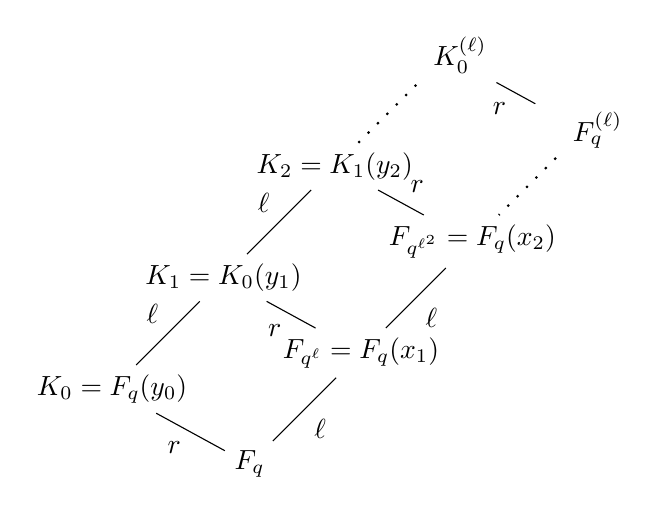
\begin{tikzpicture}[node distance=2cm]
    \node(Q){$\F_q$};
    \node(Q0)[above left =0.5cm of Q]{$\K_0=\F_q(y_0)$};
    \node(K1)[above right of=Q]{$\F_{q^\ell}=\F_q(x_1)$};
    \node(Q1)[above right of=Q0]{$\K_1=\K_0(y_1)$};
    \node(K2)[above right of=K1]{$\F_{q^{\ell^2}}=\F_q(x_2)$};
    \node(Q2)[above right of=Q1]{$\K_2=\K_1(y_2)$};
    \node(Koo)[above right of=K2]{$\quad \F_q^{(\ell)}$};
    \node(Qoo)[above right of=Q2]{$\quad\K_0^{(\ell)}$};
    \draw (Q) edge node[auto]{$r$} (Q0)
              edge node[auto, swap]{$\ell$} (K1)
          (K1) edge node[auto]{$r$} (Q1)
               edge node[auto, swap]{$\ell$} (K2)
          (Q1) edge node[auto, swap]{$\ell$} (Q0)
          (Q2) edge node[auto]{$r$} (K2)
               edge node[auto, swap]{$\ell$} (Q1)
               edge[thick, loosely dotted] (Qoo)
          (Koo) edge[thick, loosely dotted] (K2)
               edge node[auto]{$r$} (Qoo);
  \end{tikzpicture}
  \caption{The $\ell$-adic towers over $\F_q$ and $\K_0$.}
  \label{fig:ladic}
\end{figure}

We show here how to compute these polynomials, the polynomials $T_i$
of Eq.~\eqref{eq:QiTi} and how to perform lift and push.  To this
effect, we will define more general minimal polynomials: for $0 \le j
\le i$, we will let $Q_{i,j} \in \F_q(x_j)[X_i]$ be the minimal
polynomial of $x_i$ over $\F_q(x_j)$, so that $Q_{i,j}$ has degree
$\ell^{i-j}$, with in particular $Q_{i,0}=Q_i$ and
$Q_{i,i-1}=T_i(x_{i-1},X_i)$.

In Subsections~\ref{ssec:T1} and~\ref{ssec:T2}, we discuss favorable
cases, where $\ell$ divides respectively $q-1$ and $q+1$. The first
case is folklore; it yields the fastest and simplest algorithms. Our
results for the second case are related to known facts about Chebyshev
polynomials~\cite[\S~6.2]{silverman2007arithmetic}, but, to the best
of our knowledge, are new. We will revisit these cases in
Section~\ref{sec:fibers} and account for their naming convention. Our
results in the general case (Subsection~\ref{ssec:gal}) are slower,
but still quasi-linear in $\ell^i$, up to a factor polynomial in
$\ell$.


Shoup used this setup to compute $Q_i$ in time quad\-ratic in
$\ell^i$~\cite[Th.~11]{shoup94}. It is noted there that using {\em
  modular composition} techniques~\cite[Ch.~12]{vzGG}, this could be
improved to get a subquadratic exponent in $\ell^i$, up to an extra
cost polynomial in $\ell$.  For $\ell=3$ (where we are in one the
first two cases), Couveignes and Lercier make a similar remark
in~\cite[\S~2.4]{couveignes+lercier11}; using a result by Kedlaya and
Umans~\cite{KeUm11} for modular composition, they derive for any
$\varepsilon > 0$ a cost of $3^{i(1+\varepsilon)}O(\log(q))$ {\em bit}
operations, up to polynomial terms in $\log\log(q)$.

In this section, and in the rest of this paper, if $L/K$ is a field
extension, we write $\trace_{L/K}$, $\norm_{L/K}$ and $\gal_{L/K}$ for
the trace, norm and Galois group of the extension. 

%%%%%%%%%%%%%%%%%%%%%%%%%%%%%%%%%%%%%%%%%%%%%%%%%%%%%%%%%%%%

\subsection{Finding $P_0$}

To determine $P_0$, we compute the $\ell$-th cyclotomic polynomial
$\Phi_\ell \in \Z[X_0]$ and factor it over $\F_q[X_0]$:
by~\cite[Th.~9]{shoup94}, this takes $O_e(\MM(\ell)\log(\ell q))$
operations in $\F_q$.

Over $\F_q[X_0]$, $\Phi_\ell$ splits into irreducible factors of the
same degree $r$, where $r$ is the order of $q$ in $\Z/\ell\Z$ (so $r$
divides $\ell-1$); let $F_0$ be one of these factors. By construction,
there exist non $\ell$-adic residues in $\F_q[X_0]/\langle F_0
\rangle$. Once such a non-residue $y_0$ is found, we simply let $P_0$
be its minimal polynomial over $\F_q$ (which still has degree $r$);
given $y_0$, computing $P_0$ takes $O(r^2)$ operations in
$\F_q$~\cite[Th.~4]{shoup94}.

Following~\cite{Shoup90,shoup94,couveignes+lercier11}, we pick $y_0$
at random: we expect to find a non-residue after $O(1)$ trials;
by~\cite[Lemma~15]{shoup94}, each takes
$O_e(\MM(\ell)\log(r)+\MM(r)\log(\ell)\log(r)+\MM(r)\log(q))$
operations in $\F_q$. An alternative due to Lenstra and De Smit is to
take iterated $\ell$-th roots of $X_0 \bmod F_0$ until we find a
non-residue: this idea is helpful in making the construction
canonical, but more costly, so we do not consider it.

%%%%%%%%%%%%%%%%%%%%%%%%%%%%%%%%%%%%%%%%%%%%%%%%%%%%%%%%%%%%

\subsection{$\vmathbb{G}_m$-type extensions}\label{ssec:T1}


We consider here the simplest case, where $\ell$ divides $q-1$; the
(classical) facts below give the first row of Table~\ref{table:main}.
In this case, $\Phi_\ell$ splits into linear factors over $\F_q$ (so
$r=1$). The polynomial $P_0$ is of the form $Y_0-y_0$, where $y_0$ is
a non $\ell$-adic residue in $\F_q$; since we can bypass the
factorization of $\Phi_\ell$, the cost of initialization is
$O_e(\log(q))$ operations in $\F_q$. Besides, no descent is required:
for $i \ge 0$, we have $\K_i=\F_{q^{\ell^i}}$ and $x_i=y_i$; the
families of polynomials we obtain are
\begin{equation}
  \label{eq:T1}
  Q_i=X_i^{\ell^i}-y_0 \quad\text{and}\quad T_i=X_{i}^\ell-X_{i-1}.
\end{equation}
Lift and push use no operation in~$\F_q$, only exponent
arithmetic. Lift takes $F = \sum_{0 \le j < \ell^{i+1}}
f_j x_{i+1}^j$ and rewrites it as a bivariate polynomial in
$x_i,x_{i+1}$ and push does  the converse operation, 
using the rules
$$x_{i+1}^j = x_i^{\,j {\rm~div~} \ell} x_{i+1}^{\,j \bmod \ell}
\quad\text{and}\quad
x_i^e x_{i+1}^f = x_{i+1}^{e \ell + f}.$$ 

%%%%%%%%%%%%%%%%%%%%%%%%%%%%%%%%%%%%%%%%%%%%%%%%%%%%%%%%%%%%

\subsection{Chebyshev-type extensions}
\label{ssec:T2}

Consider now the case where $\ell$ divides $q+1$: then, $\Phi_\ell$
splits into quadratic factors over $\F_q$ and $r=2$. We also require
that $y_0$ has norm $1$ over $\F_q$ (see below for a discussion); we
deduce an expression for the polynomials $Q_{i,j} \in
\F_q(x_{j})[X_i]$.

\begin{proposition}
  \label{th:T2-resultant}
  For $1 \le j < i$, $Q_{i,j}$ satisfies
  \begin{equation}
    \label{eq:T2-relpols}
    Q_{i,j}(X_i) = Y^{\ell^{i-j}} + Y^{-\ell^{i-j}} - x_j \mod Y^2-X_iY+1.
  \end{equation}
\end{proposition}
\begin{proof}
  Since $\norm_{\K_0/\F_q}(y_0)=1$, $\norm_{\K_i/\F_q(x_i)}(y_i)$ is
  an $\ell^i$-th root of unity. But $\ell$ does not divide $q-1$, so
  $1$ is the only such root in $\F_q$, and by induction on $i$ it also
  is the only root in $\F_q(x_i)$; hence, the minimal polynomial of
  $y_i$ over $\F_q(x_i)$ is $Y_i^2 -x_i Y_i +1$. By composition, it
  follows that the minimal polynomial of $y_i$ over $\F_q(x_{j})$ is
  $Y_i^{2\ell^{i-j}}-x_{j} Y_i^{\ell^{i-j}}+1$. Taking a resultant to
  eliminate $Y_i$
  between these two polynomials gives the following relation between
  $x_{j}$ and $x_i$:
  \begin{equation*}
    Q_{i,j}(X_i)^2 = \mathrm{Res}_{Y_i}(Y_i^{2\ell^{i-j}}-x_{j}Y_i^{\ell^{i-j}}+1,\; Y_i^2-X_i Y_i+1).
  \end{equation*}
  By direct calculation, this is equivalent to
  Eq.~\eqref{eq:T2-relpols}.
\end{proof}

As a result, we can compute $Q_{i,j}$ in time $O(\MM(\ell^{i-j}))$
by repeated squaring, but we give a better algorithm in
Section~\ref{ssec:fibers-T2} (and show how to find a $y_0$ satisfying
the hypotheses); we leave the algorithms for lift and push to
Section~\ref{sec:lift-push}.

%%%%%%%%%%%%%%%%%%%%%%%%%%%%%%%%%%%%%%%%%%%%%%%%%%%%%%%%%%%%

\subsection{The general case}\label{ssec:gal}

Finally, we discuss the general case, with no assumption on the
behavior of $\Phi_\ell$ in $\F_q[X]$. This completes the third row of
Table~\ref{table:main}, using the bound $r\in O(\ell)$.
Because $r=[\K_0 : \F_q]$ divides $\ell-1$, it is coprime with
$\ell$. Thus, $Q_i$ remains the minimal polynomial of $x_i$ over
$\K_0$, and more generally $Q_{i,j}$ remains the minimal polynomial of
$x_i$ over $\K_{j}$; this will allow us to replace $\F_q$ by $\K_0$ as
our base field. We will measure all costs by counting operations in
$\K_0$, and we will deduce the cost over $\F_q$ by adding a factor
$O(\MM(r)\log(r))$ to account for the cost of arithmetic in $\K_0$.

For $i \ge 0$, since $\K_i=\K_0[Y_i]/\langle Y_i^{\ell^i}-y_0\rangle$,
we represent its elements on the basis $\{y_i^e \mid 0 \le e <
\ell^i\}$; e.g., $x_i$ is written as
$$
\begin{array}{ccc}
x_i &=& \sum_{0 \le j \le r-1}\ y_i^{q^{\ell^i j} \bmod \ell^i}
y_0^{q^{\ell^i j} {\rm~div~} \ell^i}. 
\end{array}
$$
Our strategy is to convert between two univariate bases of $\K_i$,
$\{y_i^e \mid 0 \le e < \ell^i\}$ and $\{x_i^e \mid 0 \le e <
\ell^i\}$. In other words, we show how to apply the isomorphism
$$\Psi_i: \K_i=\K_0[Y_i]/\langle Y_i^{\ell^i}-y_0\rangle \to
\K_0[X_i]/\langle Q_{i,0}\rangle$$ and its inverse; we will compute
the required polynomials $Q_{i,0}$ and $Q_{i,i-1}$ as a byproduct. In
a second time, we will use $\Psi_i$ to perform push and lift between
the monomial basis in $x_i$ and the bivariate basis in
$(x_{i-1},x_i)$.

We will factor $\Psi_i$ into elementary
isomorphisms
$$\Psi_{i,j}: \K_j[X_i]/\langle Q_{i,j}\rangle \to
\K_{j-1}[X_i]/\langle Q_{i,j-1}\rangle, \quad j=i,\dots,1.$$ To start
the process, with $j=i$, we let $Q_{i,i}=X_i-x_i \in \K_i[X_i]$, so
that $\K_i=\K_i[X_i]/\langle Q_{i,i} \rangle$.
Take now $j \le i$ and suppose that $Q_{i,j}$ is known. We are going to
factor $\Psi_{i,j}$ further as $\Phi''_{i,j} \circ \Phi'_{i,j} \circ
\Phi_{i,j}$, by introducing first the isomorphism
$$\varphi_j: \K_j \to \K_{j-1}[Y_j]/\langle Y_j^\ell-y_{j-1}\rangle.$$
The forward direction is a push from the monomial basis in $y_j$ to
the bivariate basis in $(y_{j-1},y_j)$ and the inverse is a lift; none
of them involves any arithmetic operation (see
Subsection~\ref{ssec:T1}).  Then, we deduce the isomorphism
$$\Phi_{i,j}: \K_j[X_i]/\langle Q_{i,j} \rangle \to
\K_{j-1}[Y_j,X_i]/\langle Y_j^\ell-y_{j-1}, Q^\star_{i,j}\rangle,$$
where $Q^\star_{i,j}$ is obtained by applying $\varphi_j$ to all
coefficients of $Q_{i,j}$. Since $\Phi_{i,j}$ consists in a
coefficient-wise application of $\varphi_j$, applying it or its
inverse costs no arithmetic operations.

Next, changing the order of $Y_j$ and $X_i$, we deduce that there
exists $S_{i,j}$ in $\K_{j-1}[X_j]$ and an isomorphism
\[
	\Phi'_{i,j}: \K_{j-1}[Y_j,X_i]/\langle Y_j^\ell-y_{j-1}, Q^\star_{i,j}\rangle
	\to \K_{j-1}[X_i, Y_j]/\langle Q_{i,j-1}, Y_j-S_{i,j}\rangle,
\]
where $\deg(Q^\star_{i,j},X_i)=\ell^{i-j}$ and
$\deg(Q_{i,j-1},X_i)=\ell^{i-j+1}$. 
\begin{lemma}
  From $Q^\star_{i,j}$, we can compute $Q_{i,j-1}$ and $S_{i,j}$ in
  $O(\MM(\ell^{i+1})\log(\ell^i))$ operations in $\K_0$.  Once this
  is done, we can apply $\Phi'_{i,j}$ or its inverse in
  $O(\MM(\ell^{i+1}))$ operations in~$\K_0$.
\end{lemma}
\begin{proof}
  We obtain $Q_{i,j-1}$ and $S_{i,j}$ from the resultant and degree-1
  subresultant of $Y_j^\ell-y_{j-1}$ and $Q^\star_{i,j}$ with respect
  to $Y_j$, computed over the polynomial ring $\K_{j-1}[X_i]$. This is
  done by the algorithms of~\cite{Reischert97,LiRo01}, using
  $O(\MM(\ell^{i+1})\log(\ell))$ operations in $\K_0$ (for this
  analysis, and all others in this proof, we assume that we use Kronecker's
  substitution for multiplications). To obtain $S_{i,j}$, we
  invert the leading coefficient of the degree-1 subresultant modulo
  the resultant $Q_{i,j-1}$; this takes
  $O(\MM(\ell^{i})\log(\ell^i))$ operations in $\K_0$.

  Applying $\Phi'_{i,j}$ amounts to taking a polynomial $A(Y_j,X_i)$ 
  reduced modulo $\langle Y_j^\ell-y_{j-1}, Q^\star_{i,j}\rangle$
  and reducing it modulo $\langle Q_{i,j-1}, Y_j-S_{i,j}\rangle$. This
  is done by computing $A(S_{i,j},X_i)$, doing all operations
  modulo $Q_{i,j-1}$. Using Horner's scheme, this takes $O(\ell)$ 
  operations $(+,\times)$ in $\K_{j-1}[X_i]/\langle Q_{i,j-1}\rangle$,
  so the complexity claim follows.

  Conversely, we start from $A(X_i)$ reduced modulo $Q_{i,j-1}$; we
  have to reduce it modulo $\langle Y_j^\ell-y_{j-1},
  Q^\star_{i,j}\rangle$. This is done using the fast Euclidean
  division algorithm with coefficients in $\K_{j-1}[Y_j]/\langle
  Y_j^\ell-y_{j-1}\rangle$ for $O(\MM(\ell^{i+1}))$
  operations in $\K_0$.
\end{proof}

The last isomorphism $\Phi''_{i,j}$ is trivial:
$$\Phi''_{i,j}: \K_{j-1}[X_i, Y_j]/\langle Q_{i,j-1}, Y_j-S_{i,j}\rangle
\to \K_{j-1}[X_i]/\langle Q_{i,j-1}\rangle$$
forgets the variable $Y_j$; it requires no arithmetic operation.

Taking $j=i,\dots,1$ allows us to compute $Q_{i,i-1}$ and $Q_{i,0}$
for $O(i^2\MM(\ell^{i+1})\log(\ell))$ operations in $\K_0$. Composing
the maps $\Psi_{i,j}$, we deduce further that we can apply $\Psi_i$ or
its inverse for $O(i\MM(\ell^{i+1}))$ operations in $\K_0$.  

We claim that we can then perform push and lift between the monomial
basis in $x_i$ and the bivariate basis in $(x_{i-1},x_i)$ for the same
cost. Let us for instance explain how to lift.

We start from $A$ written on the bivariate basis in $(x_{i-1},x_i)$;
that is, $A$ is in $\K_0[X_{i-1},X_i]/\langle Q_{i-1},
T_{i}\rangle$. Apply $\Psi_{i-1}$ to its coefficients in
$x_i^0,\dots,x_i^{\ell-1}$, to rewrite $A$ as an element of
$$\K_0[Y_{i-1},X_i]/\langle Y_{i-1}^{\ell^{i-1}}-y_{i-2},
T_{i}\rangle = \K_{i-1}[X_i]/\langle Q_{i,i-1} \rangle.$$ Applying
$\Psi_{i,i}^{-1}$ gives us the image of $A$ in $\K_i$, and applying
$\Psi_i$ finally brings it to $\K_0[X_i]/\langle Q_{i}\rangle$.


%%%%%%%%%%%%%%%%%%%%%%%%%%%%%%%%%%%%%%%%%%%%%%%%%%%%%%%%%%%%
%%%%%%%%%%%%%%%%%%%%%%%%%%%%%%%%%%%%%%%%%%%%%%%%%%%%%%%%%%%%
%%%%%%%%%%%%%%%%%%%%%%%%%%%%%%%%%%%%%%%%%%%%%%%%%%%%%%%%%%%%

\section{Towers from irreducible fibers}
\label{sec:fibers}

In this section we discuss another construction of the $\ell$-adic
tower based on work of Couveignes and
Lercier~\cite{couveignes+lercier11}. The results of this section are
summarized in rows 2, 4 and 5 of Table~\ref{table:main}. This
construction is not unrelated to the ones of the previous section, and
indeed we will start by showing how those of Sections~\ref{ssec:T1}
and~\ref{ssec:T2} reduce to it.

Here is the bottom line of Couveignes' and Lercier's idea. Let $G, G'$
be integral algebraic $\F_q$-groups of the same dimension and let $\phi:
G' \rightarrow G$ be a surjective, separable algebraic group morphism.
Let $\ell$ be the degree of $\phi$; then, the set of points $x \in G$
with fiber $G'_x$ of cardinality $\ell$ is a nonempty open subset $U
\subset G$. If the induced homomorphism $G'(\F_q) \rightarrow G(\F_q)$
of groups is not surjective then there are points of $G(\F_q)$ with
fibers lying in algebraic extensions of $\F_q$. Assume that we are
able to choose $\phi$ so that we can find one of these points contained
in $U$, with an irreducible fiber, and apply a linear projection to
this fiber (e.g., onto an axis). The resulting polynomial is
irreducible of degree dividing $\ell$ (and expectedly equal to
$\ell$). If we can repeat the construction with a new map $\phi':G''\to
G'$, and so on, the sequence of extensions makes an $\ell$-adic tower
over $\F_q$.

%%%%%%%%%%%%%%%%%%%%%%%%%%%%%%%%%%%%%%%%%%%%%%%%%%%%%%%%%%%%

\subsection{Towers from algebraic tori}
\label{ssec:fibers-T2}
In~\cite{couveignes+lercier11}, Couveignes and Lercier explain how
their idea yields the tower of Section~\ref{ssec:T1}. Consider the
multiplicative group $\vmathbb{G}_m$: this is an algebraic group of
dimension one, and $\vmathbb{G}_m(\F_q)$ has cardinality $q-1$.  The
$\ell$-th power map defined by $\phi:X\mapsto X^\ell$ is a degree
$\ell$ algebraic endomorphism of $\vmathbb{G}_m$, surjective over the
algebraic closure.

Suppose that $\ell$ divides $q-1$, and let $\eta$ be a non $\ell$-adic
residue in $\F_q$ ($\eta$ plays here the same role as $y_0$ in
Section~\ref{sec:LDtower}). For any $i>0$, the fiber $\phi^{-i}(\eta)$
is defined by $X^{\ell^i}-\eta$: we recover the construction of
Subsection~\ref{ssec:T1}.

More generally, following~\cite{rubin+silverberg03,voskresenskii98},
we let $k=\F_q$, $L=\F_{q^n}$ and $k\subset F\subsetneq L$. The Weil
restriction $\Res_{L/k}\vmathbb{G}_m$ is an \emph{algebraic torus}, and
the norm $\norm_{L/F}$ induces a map
$\Res_{L/k}\vmathbb{G}_m\to\Res_{F/k}\vmathbb{G}_m$. Define the
\emph{maximal torus} $\vmathbb{T}_n$ as the intersection of the kernels of the
maps $\norm_{L/F}$ for all subfields $F$. Then $\vmathbb{T}_n$ has dimension
$\varphi(n)$, is isomorphic to $\vmathbb{G}_m^{\varphi(n)}$ over the
algebraic closure, and its $k$-rational points form a group of
cardinality $\Phi_n(q)$:
\begin{equation}
  \label{eq:Tn}
  \vmathbb{T}_n(k) \cong \{\alpha\in L^\ast \;|\; \norm_{L/F}(\alpha) = 1 
  \text{ for all $k\subset F\subsetneq L$} \}.
\end{equation}


We now detail how the construction of Section~\ref{ssec:T2} can be
obtained by considering the torus $\vmathbb{T}_2$; this will allow us to start
completing the second row in Table~\ref{table:main}.

\begin{lemma}
  Let $\Delta\in\F_q$ be a quadratic non-residue if $p\ne2$, or such
  that $\trace_{\F_q/\F_2}(\Delta)=1$ otherwise. Let $\delta=\sqrt{\Delta}$
  or $\delta^2+\delta=\Delta$ accordingly. The
  maximal torus $\vmathbb{T}_2$ is isomorphic to the \emph{Pell conic}
  \begin{equation}
    \label{eq:Pell}
    C \;:\; 
    \begin{cases}
      x^2 - \Delta y^2 = 4 &\text{if $p\ne2$,}\\
      x^2\Delta + xy + y^2 = 1 &\text{if $p=2$.}
    \end{cases}
  \end{equation}
  Multiplication in $\vmathbb{T}_2$ induces a group law on $C$. The neutral
  element is $(2,0)$ if $p\ne2$, or $(0,1)$ if $p=2$. The sum of two
  points $P=(x_1,y_1)$ and $Q=(x_2,y_2)$ is defined
  by
  \begin{equation*}
    P\oplus Q =
    \begin{cases}
      \displaystyle
      \left(\frac{x_1x_2 + \Delta y_1y_2}{2},\; \frac{x_1y_2 + x_2y_1}{2}\right) &
      \text{if $p\ne2$,}\\
      \left(x_1x_2 + x_1y_2 + x_2y_1,\; x_1x_2\Delta + y_1y_2\right) &
      \text{if $p=2$.}
    \end{cases}
  \end{equation*}
\end{lemma}
\begin{proof}
  The isomorphism follows by Weil restriction to $\F_q(\delta)/\F_q$
  with respect to the basis $(1/2,\delta/2)$ if $p\ne2$, or
  $(\delta,1)$ if $p=2$. Indeed, by virtue of Eq.~\eqref{eq:Tn}, an
  element $(x,y)$ of $\F_q(\delta)$ belongs to $\vmathbb{T}_2$ if and only if
  its norm over $\F_q$ is $1$.
  Let $\sigma$ be the generator of $\gal_{\F_q(\delta)/\F_q}$. For
  $p\neq2$, clearly $\delta^\sigma=-\delta$. For $p=2$, by
  Artin-Schreier theory,
  $\trace_{\F_q(\delta)/\F_q}(\delta)=\trace_{\F_q/\F_2}(\Delta)=1$, hence
  $\delta^\sigma=1+\delta$. In both cases, Eq.~\eqref{eq:Pell}
  follows.  The group law is obtained by direct calculation.
\end{proof}

Pell conics are a classic topic in number theory\cite{lenstra02-pell}
and computer science, with applications to primality proving,
factorization~\cite{lemmermeyer03,hambleton12} and
cryptography~\cite{rubin-silverberg+crypto03}. 

As customary, we denote by $[n](x,y)$ the $n$-th scalar multiple of a
point $(x,y)$.  $[n]$ is an endomorphism of $C$ of degree
$n$, separable if and only if $(n,p)=1$.

\begin{lemma}
  \label{th:T2-divpol}
  Let $P=(\alpha,\beta)$ be a point of $C$. The abscissa of $[n]P$ is
  given by $C_n(\alpha)$, where $C_n\in\Z[X]$ is the $n$-th Chebyshev
  polynomial, defined by $C_0=2$, $C_1=X$, and
  \begin{equation}
    \label{eq:Chebyshev}
    C_{n+1} = XC_n - C_{n-1}.
  \end{equation}
\end{lemma}
\begin{proof}
  Induction on $n$. A detailed proof can be found in
  \cite[Prop.~6.6]{silverman2007arithmetic}.
\end{proof}


%%%%%%%%%%%%%%%%%%%%%%%%%%%%%%%%%%%%%%%%%%%%%%%%%%%%%%%%%%%%



\begin{theorem}
  \label{th:T2-irred}
  Let $\eta\in\F_q(\delta)$ be a non $\ell$-adic residue in $\vmathbb{T}_2$, and
  let $P=(\alpha,\beta)$ be its image in $C/\F_q$. For any $i>0$, the
  polynomials $C_{\ell^i}-\alpha$ are irreducible. Their roots are the
  abscissas of the images in $C/\F_{q^{\ell^i}}$ of the $\ell^i$-th
  roots of $\eta$.
\end{theorem}
\begin{proof}
  By~\cite[Th.~VI.9.1]{lang}, the polynomial $X^{\ell^i}-\eta$ is
  irreducible. Its roots correspond to the fiber $[\ell^i]^{-1}(P)$,
  and the Galois group of $\F_{q^{\ell^i}}/\F_q$ acts transitively on
  them.

  Two points of $C$ have the same abscissa if and only if they are
  opposite. But $\eta$ is a non $\ell$-adic residue, hence
  $\eta\ne\eta^{-1}$, and all the points in $[\ell^i]^{-1}(P)$ have
  distinct abscissa.  By Lemma~\ref{th:T2-divpol}, $C_{\ell^i}-\alpha$
  vanishes precisely on those abscissas and is thus irreducible.
\end{proof}

We can now apply our results to the computation of the polynomials
$Q_i$ and $T_i$ of Section~\ref{ssec:T2}.

\begin{corollary}
  The polynomials $Q_{i,j}$ of Prop.~\ref{th:T2-resultant}
  satisfy
  \begin{equation*}
    Q_{i,j}(X_i) = C_{\ell^{i-j}}(X_i) - x_j.
  \end{equation*}
\end{corollary}
\begin{proof}
  We have already shown that $\norm_{\K_j/\F_q(x_j)}(y_j)=1$ for any
  $j$, thus $y_j$ is a non $\ell$-adic residue in
  $\vmathbb{T}_2/\F_q(x_j)$. Independently of the characteristic and of the
  element $\Delta\in\F_q(x_j)$ chosen, the abscissa of the image of
  $y_j$ in $C/\F_q(x_j)$ is $\trace_{\K_j/\F_q(x_j)}y_j=x_j$. The
  statement follows from the previous theorem.
\end{proof}

There is a folklore algorithm computing the $n$-th Chebyshev
polynomial using $O(n)$ operations in
$\Z$~\cite{koepf1999chebyshev}. We shall need a slightly better
algorithm working modulo $p$.

\begin{corollary}
  The polynomials $Q_{i,j}$ can be computed using $O(\ell^{i-j})$
  operations in $\F_p$.
\end{corollary}
\begin{proof}
  Let $C_n = \sum_i c_{n,i}X^{n-i}$. It is well known that $\lvert
  c_{n+k,2k}\rvert$ are the coefficients of the $(1,2)$-Pascal
  triangle, also called Lucas' triangle
  (see~\cite[Prop.~6.6]{silverman2007arithmetic}
  and~\cite{benjamin10}). It follows that
  \begin{equation*}
    \frac{c_{n,2k+2}}{c_{n,2k}} = 
    -\frac{(n-2k)(n-2k-1)}{(n-k-1)(k+1)},
  \end{equation*}
  which immediately gives the algorithm. Indeed, since we know the
  $c_{n,2k}$'s are the image mod $p$ of integers, we compute them
  using multiplications and divisions in $\Q_p$ with relative
  precision 1.
\end{proof}

We are left with the problem of finding the non $\ell$-adic residue
$\eta$ to initialize the tower. As before, this will be done by random
sampling and testing.

\begin{lemma}
  \label{th:montgomery}
  Let $P=(\alpha,\beta)$ be a point on $C$. For any $n$, there is a
  formula to compute the abscissa of $[\pm n]P$, using $O(\log n)$
  operations in $\F_q$, and not involving $\beta$.
\end{lemma}
\begin{proof}
  Observe that if $n=2$, the abscissa of $[\pm 2]P$ is $\alpha^2-2$
  (for any $p$).  Let $P'=(\alpha',\beta')$, and let $\gamma$ be the
  abscissa of $P\ominus P'$. By direct computation we find that the
  abscissa of $P\oplus P'$ is $\alpha\alpha'-\gamma$ (for any $p$);
  this formula is called a \emph{differential addition}.  Thus, $O(1)$
  operations are needed for a doubling or a differential addition. To
  compute the abscissa of $[\pm n]P$, we use the ladder algorithm
  of~\cite{montgomery}, requiring $O(\log n)$ doublings and
  differential additions.
\end{proof}

\begin{proposition}
  The abscissa of a point $P\in C/\F_q$ satisfying the
  conditions of Theorem~\ref{th:T2-irred} can be found using $O_e(\log
  q)$ operations in $\F_q$.
\end{proposition}
\begin{proof}
  We randomly select $\alpha\in\F_q$ and test that it belongs to
  $C$. If $p\ne2$, this amounts to testing that $\alpha^2-4$ is a
  quadratic non-residue in $\F_q$, a task that can be accomplished
  with $O(\log q)$ operations. If $p=2$, by Artin-Schreier theory this
  is equivalent to $\trace_{\F_q/\F_2}(1/\alpha^2)=1$, which can be
  tested in $O(\log q)$ operations in $\F_q$.

  Then we check that $P$ is a non $\ell$-adic residue by verifying
  that $[(q+1)/\ell]P$ is not the group identity. By
  Lemma~\ref{th:montgomery}, this computation requires $O(\log q)$
  operations.
  About half of the points of $\F_q$ are quadratic non-residues, and
  about $1-1/\ell$ of them are the abscissas of points with the
  required order, thus we expect to find the required element after
  $O_e(1)$ trials.
\end{proof}

It is natural to ask whether a similar construction could be applied
to any $\ell$. If $r$ is the order of $q$ modulo $\ell$, the natural
object to look at is $\vmathbb{T}_r$, but here we are faced with two
problems. First, multiplication by $\ell$ is now a degree
$\ell^{\varphi(r)}$ map, thus its fibers have too many points; instead,
isogenies of degree $\ell$ should be considered. Second, it is an open
question whether $\vmathbb{T}_r$ can be parameterized using $\varphi(r)$
coordinates; but even assuming it can be, we are still faced with the
computation of a univariate annihilating polynomial for a set embedded
in a $\varphi(r)$-dimensional space, a problem not known to be feasible
in quasi-linear time. Studying this generalization is another natural
follow-up to the present work.

%%%%%%%%%%%%%%%%%%%%%%%%%%%%%%%%%%%%%%%%%%%%%%%%%%%%%%%%%%%%

\subsection{Towers from elliptic curves}
\label{sec:elliptic}

Since it seems hard to deal with higher dimensional algebraic tori, it
is interesting to look at other algebraic groups. Being
one-dimensional, elliptic curves are good candidates. In this
section, we quickly review Couveignes' and Lercier's construction,
referring to~\cite{couveignes+lercier11} for details, and point out
the modifications needed in order to build towers (as opposed to
constructing irreducible polynomials).

\begin{figure}[t]
  \centering
  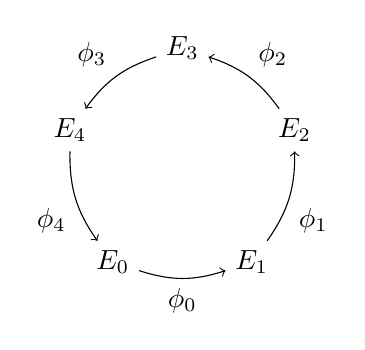
\begin{tikzpicture}
    \def\n{4}
    \foreach \i in {0,...,\n} {
      \pgfmathparse{360/(\n+1)*(\i-1/2) - 90}
      \let\angle\pgfmathresult
      \draw (\angle:1.5) node (E\i) {$E_\i$};
    }
    \foreach \i in {0,...,\n} {
      \pgfmathparse{int(mod(\i+1, \n+1))}
      \let\j\pgfmathresult
      \draw (E\i) edge[->,bend right=18] node[auto,swap] {$\phi_\i$} (E\j);
    }
  \end{tikzpicture}
  \caption{The isogeny cycle of $E_0$.}
  \label{fig:volcano}
\end{figure}

Let $\ell$ be a prime different from $p$ and not dividing $q-1$. Let
$E_0$ be an elliptic curve whose cardinality over $\F_q$ is a multiple
of $\ell$. By Hasse's bound, this is only possible if $\ell\le q +
2\sqrt{q} + 1$.  An \emph{isogeny} is an algebraic group morphism
between two elliptic curves that is surjective in the algebraic
closure. It is said to be rational over $\F_q$ if it is invariant
under the $q$-th power map; such an isogeny exists if and only if the
curves have the same number of points over $\F_q$. An isogeny of
degree $n$ is separable if and only if $n$ is prime to $p$, in which
case its kernel contains exactly $n$ points.  Because of the
assumptions on $\ell$, there exists an $e\ge1$ such that, for any
curve $E$ isogenous to $E_0$, the $\F_q$-rational part of $E[\ell]$ is
cyclic of order $\ell^e$.

Suppose for simplicity, that $p\ne2,3$ and let $E_0$ be expressed as
the locus
\begin{equation}
  E_0 \;:\; y^2 = x^3 + ax + b,
  \quad\text{with $a,b\in\F_q$},
\end{equation}
plus one point at infinity.  We denote by $H_0$ the unique subgroup of
$E_0/\F_q$ of order $\ell$, and by $\phi_0$ the unique isogeny whose
kernel is $H_0$; we then label $E_1$ the image curve of $\phi_0$. We
go on denoting by $H_i$ the unique subgroup of $E_i/\F_q$ of order
$\ell$, and by $\phi_i:E_i\to E_{i+1}$ the unique isogeny with kernel
$H_i$. The construction is depicted in Figure~\ref{fig:volcano}.

\begin{lemma}
  \label{th:class-number}
  Let $E_0,E_1,\dots$ be defined as above, there exists $n\in
  O(\sqrt{q}\log (q))$ such that $E_n$ is isomorphic to $E_0$.
\end{lemma}
\begin{proof}
  It is shown in \cite[\S~4]{couveignes+lercier11} that the
  isogenies $\phi_i$ are \emph{horizontal} in the sense
  of~\cite{kohel}, hence they necessarily form a cycle. Let $t$ be the
  trace of $E_0$, the length of the cycle is bounded by the class
  number of $\Q[X]/(X^2-tX-q)$, thus by Minkowski's bound it is in
  $O(\sqrt{q}\log (q))$.
\end{proof}

In what follows, the index $i$ is to be understood modulo the length of
the cycle. This is a slight abuse, because $E_n$ is isomorphic but not
equal to $E_0$, but it does not hide any theoretical or computational
difficulty.

Under the former assumptions, it is proved
in~\cite[\S~4]{couveignes+lercier11} that if $P$ is a point of
$E_i$ of order divisible by $\ell^e$, if
$\psi=\phi_{i-1}\circ\phi_{i-2}\circ\cdots\circ\phi_{j}$, then the
fiber $\psi^{-1}(P)$ is irreducible and has cardinality $\ell^{i-j}$.
Knowing $E_i$, Vélu's formulas~\cite{velu71} allow us to express the
isogenies $\phi_i$ as rational fractions
\begin{equation}
  \begin{aligned}
    \phi_i: E_i &\to E_{i+1},\\
    (x,y) &\mapsto \left(\frac{f_i(x)}{g_i(x)}, y\left(\frac{f_i(x)}{g_i(x)}\right)'\right),
  \end{aligned}
\end{equation}
where $g_i$ is the square polynomial of degree $\ell-1$ vanishing on
the abscissas of the affine points of $H_i$, and $f_i$ is a polynomial
of degree $\ell$. 

There is a subtle difference between our setting and Couveignes' and
Lercier's. The goal of~\cite{couveignes+lercier11} is to compute an
extension of degree $\ell^i$ of $\F_q$ for a fixed $i$: this can be
done by going forward $i$ times, then taking the fiber of a point of $E_i$ by
the isogenies $\phi_{i-1}, \ldots, \phi_0$. In our case, we are
interested in building extensions of degree $\ell^i$
\emph{incrementally}, i.e.\ without any \emph{a priori} bound on
$i$. Thus, we have to walk \emph{backwards} in the isogeny cycle: if
$\eta\in\F_q$ is the abscissa of a point of $E_0$ of order $\ell^e\ne
2$, we will use the following polynomials to define the $\ell$-adic
tower:
\begin{align*}
  T_1 &= f_{-1}(X_1) - \eta g_{-1}(X_1),\\ 
  T_i &= f_{-i}(X_i) - X_{i-1} g_{-i}(X_i).
\end{align*}

The following theorem gives the time for building the tower; lift and
push are detailed in the next section. 

\begin{theorem}\label{theo:elliptic}
  Suppose $4\ell\le q^{\sfrac{1}{4}}$, and under the above assumption.
  Initializing the $\ell$-adic tower requires
  $O\tilde{_e}(\ell\log^5(q)+\ell^3)$ bit operations; and building the
  $i$-th level requires $O_e(\ell^2+\MM(\ell)\log(\ell
  q)+\MM(\ell^i)\log(\ell^i))$ operations in~$\F_q$.
\end{theorem}
\begin{proof}
  For the initialization, \cite[\S~4.3]{couveignes+lercier11}
  shows that if $4\ell\le q^{\sfrac{1}{4}}$, a curve $E_0$ with the required
  number of points can be found in $O\tilde{_e}(\ell\log^5(q))$ bit
  operations. We also need to compute the $\ell$th modular polynomial
  $\Phi_\ell\bmod p$; for this, we compute it over $\Z$ with
  $\tildO(\ell^3)$ bit operations~\cite{enge09}, then reduce it
  modulo $p$.

  To build the $i$-th level, we first need to find the equation of
  $E_{-i}$. For this, we evaluate $\Phi_\ell$ at $j(E_{-i+1})$, using
  $O(\ell^2)$ operations. Lemma~\ref{th:class-number} implies that
  this polynomial has only two roots in $\F_q$, namely $j(E_{-i})$ and
  $j(E_{-i+2})$. We factor it using $O_e(\MM(\ell)\log(\ell q))$
  operations~\cite[Ch~14]{vzGG}, and we take an arbitrary curve with
  $j$-invariant $j(E_{-i})$. Then we find an $\ell$-torsion point
  using $O_e(\log q)$ operations, and apply Vélu's formulas to compute
  $\phi_{-i}$. We deduce the polynomial $T_i$, and $Q_i$ is obtained
  using $O(\MM(\ell^i)\log(\ell^i))$ operations using
  Algorithm~\ref{alg:compose} given in the next section.
\end{proof}

\begin{remark}
  \label{rk:elliptic}
  Instead of computing the cycle step by step, we could compute it
  entirely during the initialization phase, by using Vélu's formulas
  alone to compute $E_1,E_2,\dots$ until we hit $E_0$ again. By doing
  so, we avoid using the modular polynomial $\Phi_\ell$ at each new
  level. By Lemma~\ref{th:class-number}, this requires
  $O_e(\ell\sqrt{q}\log(q))$ operations. This is not asymptotically good
  in $q$, but for practical values of $q$ and $\ell$ the cycle is often
  small and this approach works well. This is accounted for in the last
  row of Table~\ref{table:main}.  
\end{remark}

%%%%%%%%%%%%%%%%%%%%%%%%%%%%%%%%%%%%%%%%%%%%%%%%%%%%%%%%%%%%
%%%%%%%%%%%%%%%%%%%%%%%%%%%%%%%%%%%%%%%%%%%%%%%%%%%%%%%%%%%%
%%%%%%%%%%%%%%%%%%%%%%%%%%%%%%%%%%%%%%%%%%%%%%%%%%%%%%%%%%%%

\section{Lifting and pushing}
\label{sec:lift-push}

The previous constructions of $\ell$-adic towers based on irreducible
fibers share a common structure that allows us to treat lifting and
pushing in a unified way. Renaming the variables $(X_{i-1},X_i)$ as
$(X,Y)$, the polynomials $(Q_{i-1},Q_i,T_i)$ as $(R,S,T)$, the
extension at level $i$ is described as
$$\F_q[Y]/ \langle S(Y) \rangle \quad\text{and}\quad \F_q[X,Y]/\langle
R(X), T(X,Y) \rangle,$$ with $R$ of degree $\ell^{i-1}$, $S$ of degree
$\ell^i$, and where $T(X,Y)$ has the form $f(Y)-X g(Y)$, with $\deg(f)
=\ell$, $\deg(g) < \ell$ and $\gcd(f,g)=1$; possibly, $g=1$. In all
this section, $f$, $g$ and their degree $\ell$ are fixed.

Lift is the conversion from the bivariate basis associated to the
right-hand side to the univariate basis associated to the left-hand side;
push is the inverse. Using the special shape of the polynomial $T$,
they reduce to composition and decomposition of rational functions, as
we show next. These results fill in all missing entries in the lift / push 
column of Table~\ref{table:main}.


%%%%%%%%%%%%%%%%%%%%%%%%%%%%%%%%%%%%%%%%%%%%%%%%%%%%%%%%%%%%

\subsection{Lifting}

Let $P$ be in $\F_q[X,Y]$ and $n$ be in $\N$, with $\deg(P,X)< n$. We
define $P[f,g,n]$ as
$$P[f,g,n] = g^{n-1} P\left (\frac fg, Y\right) \in \F_q[X,Y].$$ If
$P=\sum_{i=0}^{n-1} p_i(Y) X^i$, then $P[f,g,n] = \sum_{i=0}^{n-1}
p_if^ig^{n-1-i}$.  We first give an algorithm to compute this
expression, then show how to relate it to lifting; when $g=1$,
Algorithm~\ref{alg:compose} reduces to a well known algorithm for
polynomial composition~\cite[Ex.~9.20]{vzGG}.

\begin{algorithm}[Compose]
  \label{alg:compose}
  \begin{algorithmic}[1]
    \REQUIRE $P\in \F_q[X,Y]$, $f,g\in \F_q[Y]$, $n\in\N$
    \IF {$n = 1$} 
    \RETURN $P$
    \ELSE
    \STATE $m \leftarrow \lceil n/2\rceil$
    \STATE Let $P_0,P_1$ be such that $P = P_0 + X^mP_1$
    \STATE $Q_0 \leftarrow$ Compose($P_0, f, g, m$)
    \STATE $Q_1 \leftarrow$ Compose($P_1, f, g, n-m$)
    \STATE $Q \leftarrow Q_0g^{n-m} + Q_1f^m$  \label{alg:compose:res}
    \RETURN $Q$
    \ENDIF
  \end{algorithmic}
\end{algorithm}

\begin{theorem}
  \label{th:compose}
  On input $P,f,g,n$, with $\deg(P,X)<n$ and $\deg(P,Y) < \ell$,
  Algorithm~\ref{alg:compose} computes $Q=P[f,g,n]$ using $O(\MM(\ell
  n)\log(n))$ operations in $\F_q$.
\end{theorem}
\begin{proof}
  If $n=1$, the theorem is obvious. Suppose $n>1$, then $P_0$ and
  $P_1$ have degrees less than $m$ and $n-m$ respectively. By
  induction hypothesis,
  \begin{align*}
      & Q_0 = P_0[f,g,m] = \sum_{i=0}^{m-1}p_if^ig^{m-1-i},\\
      & Q_1 = P_1[f,g,n-m] = \sum_{i=0}^{n-m-1}p_{i+m}f^ig^{n-m-1-i}.   
  \end{align*}
  Hence,
  \[
    Q = \sum_{i=0}^{m-1}p_if^ig^{n-1-i} + \sum_{i=0}^{n-m-1}p_{i+m}
    f^{i+m}g^{n-m-1-i} = P[f,g,n].
  \]
  The only step that requires a computation is
  Step~\ref{alg:compose:res}, costing $O(\MM(\ell n))$ operations in
  $\F_q$. The recursion has depth $\log(n)$, hence the overall
  complexity is $O(\MM(\ell n)\log(n))$.
\end{proof}

\begin{corollary}
  At level $i$, one can perform the lift operation using
  $O(\MM(\ell^i)\log(\ell^i))$ operations in $\F_q$.
\end{corollary}
\begin{proof}
  We start from an element $\alpha$ written on the bivariate basis, that
  is, represented as $A(X,Y)$ with $\deg(A,X)<n=\ell^{i-1}$ and
  $\deg(A,Y)<\ell$ (note that $\ell n =\ell^i$).  We compute the
  univariate polynomials $A^\star=A[f,g,n]$ and $\gamma=g^{n-1}$ using
  $O(\MM(\ell^i)\log(\ell^i))$ operations in $\F_q$; then the lift
  of $\alpha$ is $A^\star/\gamma$ modulo $S$. The inverse of $\gamma$
  is computed using $O(\MM(\ell n)\log(\ell n))$ operations, and the
  multiplication adds an extra $O(\MM(\ell n))$.
\end{proof}

%%%%%%%%%%%%%%%%%%%%%%%%%%%%%%%%%%%%%%%%%%%%%%%%%%%%%%%%%%%%

\subsection{Pushing}

We first deal with the inverse of the question dealt with in
Theorem~\ref{th:compose}: starting from $Q \in \F_q[Y]$, reconstruct
$P \in \F_q[X,Y]$ such that $Q=P[f,g,n]$. When $g=1$,
Algorithm~\ref{alg:decompose} reduces to Algorithm~9.14
of~\cite{vzGG}.

\begin{algorithm}[Decompose]
  \label{alg:decompose}
  \begin{algorithmic}[1]
    \REQUIRE $Q,f,g,h\in \F_q[Y]$, $n \in \N$ 
    \IF {$n=1$} 
    \RETURN $Q$
    \ELSE 
    \STATE $m \leftarrow \lceil n/2 \rceil$ 
    \STATE $u \leftarrow 1/ g^{n-m}\bmod f^m$ \label{alg:decompose:xgcd} 
    \STATE $Q_0 \leftarrow Q u \bmod f^m$ 
    \STATE $Q_1 \leftarrow (Q-Q_0 g^{n-m}) {\rm~div~} f^m$ 
    \STATE $P_0 \leftarrow$ Decompose($Q_0, f, g, h, m$) 
    \STATE $P_1 \leftarrow$ Decompose($Q_1, f, g, h, n-m$) 
    \RETURN $P_0 + X^m P_1$ 
    \ENDIF
  \end{algorithmic}
\end{algorithm}

\begin{theorem}
  On input $Q,f,g,h,n$, with $\deg(Q) < \ell n$ and $h = 1/g \bmod f$,
  Algorithm~\ref{alg:decompose} computes a polynomial $P\in \F_q[X,Y]$
  such that $\deg(P,X)<n$, $\deg(P,Y) <\ell$ and $Q=P[f,g,n]$ using
  $O(\MM(\ell n)\log(n))$ operations in $\F_q$.
\end{theorem}
\begin{proof}
  We prove the theorem by induction. If $n=1$, the statement is
  obvious, so let $n> 1$. The polynomials $Q_0$ and $Q_1$ verify $Q =
  Q_0g^{n-m} + Q_1f^m.$ By construction, $Q_0$ has degree less than $\ell
  m$. Since $\deg(g) < \ell$, this implies that $Q_0 g^{n-m}$ has
  degree less than $\ell n$; thus, $Q_1$ has degree less than $\ell
  (n-m)$. By induction, $P_0$ and $P_1$ have degree less than $m$,
  resp. $n-m$, in $X$, and less than  $\ell$ in $Y$, and
  \begin{align*}
      & Q_0 = P_0[f,g,m] = \sum_{i=0}^{m-1} p_{0,i}f^ig^{m-1-i}, \\
      & Q_1 = P_1[f,g,n-m] = \sum_{i=0}^{n-m-1} p_{1,i}f^ig^{n-m-1-i}.
  \end{align*}
  Hence, $P=P_0+X^mP_1$ has degree less than $n$ in $X$ and less than $\ell$ 
  in $Y$, and the following proves correctness:
  \begin{align*}
    P[f,g,n] & = \sum_{i=0}^{m-1}p_{0,i}f^ig^{n-1-i} + 
    \sum_{i=m}^{n-1}p_{1,i-m}f^ig^{n-1-i} \\
    & = P_0[f,g,m]g^{n-m} + P_1[f,g,n-m]f^m  \\
    & = Q.
  \end{align*}
  At Step~\ref{alg:decompose:xgcd}, we do as follows: starting from
  $h=1/g \bmod f$, we deduce $1/g^{n-m} \bmod f$ in time
  $O(\MM(\ell)\log(n))$ by binary powering mod $f$. We also compute
  $g^{n-m}$ in time $O(\MM(\ell n))$ by binary powering, and we use
  Newton iteration (starting from $1/g^{n-m} \bmod f$) to deduce
  $1/g^{n-m} \bmod f^m$ in time $O(\MM(\ell n))$. All other steps
  cost $O(\MM(\ell n))$; the recursion has depth $\log(n)$,
  so the total cost is $O(\MM(\ell n)\log(n))$.
\end{proof}

\begin{corollary}
  At level $i$, one can perform the push operation using
  $O(\MM(\ell^i)\log(\ell^i))$ operations in $\F_q$.
\end{corollary}
\begin{proof}
  Given $\alpha$ represented by a univariate polynomial $A(Y)$ of
  degree less than $\ell n$, with $n =\ell^{i-1}$. We compute
  $g^{n-1}$ and $A^\star = g^{n-1} A \bmod S$ using $O(\MM(\ell^i))$
  operations. Then, we compute $h=1/g \bmod f$ in time
  $O(\MM(\ell)\log(\ell))$ and apply Algorithm~\ref{alg:decompose}
  to $A^\star$, $f$, $g$, $h$ and $n$. The result is a bivariate
  polynomial $B$, representing $\alpha$ on the bivariate basis. The
  dominant phase is Algorithm~\ref{alg:decompose}, costing
  $O(\MM(\ell^i)\log(\ell^i))$ operations in $\F_q$.
\end{proof}

%%%

\section{Implementation}
\label{sec:impl}
To demonstrate the interest of our constructions, we made a very basic
implementation of the towers of Sections~\ref{ssec:fibers-T2}
and~\ref{sec:elliptic} in Sage~\cite{Sage}. It relies on Sage's
default implementation of quotient rings of $\F_p[X]$, which itself
uses NTL \cite{shoup2003ntl} for $p=2$ and FLINT~\cite{hart2010flint}
for other primes. Towers based on elliptic curves are constructed
using the algorithm described in Remark~\ref{rk:elliptic}. The source
code is available at \url{http://defeo.github.io/towers}

We compare our implementation to three ways of constructing
$\ell$-adic towers in Magma. First, one may construct the levels from
bottom to top using the finite field constructor \verb+GF()+. For the
parameters we used, Magma uses tables of precomputed
Conway polynomials and automatically computes embeddings on creation,
see~\url{http://magma.maths.usyd.
  edu.au/magma/releasenotes/2/14}. The second approach constructs the
highest level of the tower first, then all the lower levels using the
\verb+sub<>+ constructor. The last one constructs the levels from
bottom to top using random dense polynomials and calls the
\verb+Embed()+ function; we do not count the time for finding the
irreducible polynomials.

\begin{figure}[h]
  \centering
  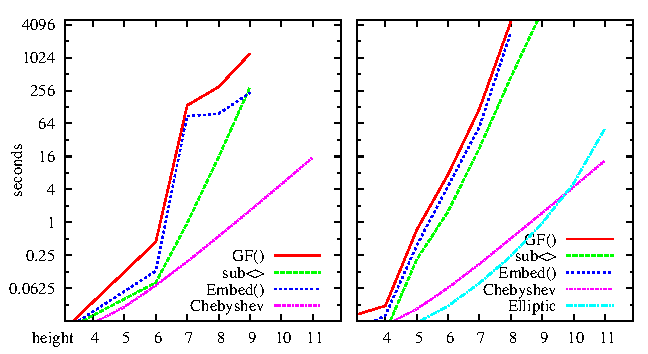
\includegraphics[width = 10cm]{creat}
  \caption{Times for building $3$-adic towers on top of $\F_2$ (left)
    and $\F_5$ (right), in Magma (first three lines) and using our
    code.}
  \label{fig:build}
\end{figure}

We ran tests on an Intel Xeon E5620 clocked at 2.4 GHz, using Sage 5.5
and Magma 2.18.12. The time required for the creation of $3$-adic
towers of increasing height is summarized in
Figure~\ref{fig:build}; the timings of our algorithms are labeled 
Chebyshev and Elliptic. Computations that took more than 4GB RAM were
interrupted.

Despite its simplicity, our code consistently outperforms Magma on
creation time. On the other hand, lift and push operations take
essentially no time in Magma, while in all the tests of
Figure~\ref{fig:build} we measured a running time almost perfectly
linear for one push followed by one lift, taking approximately $70\mu
s$ per coefficient (this is in the order of a second around level
10). Nevertheless, the large gain in creation time makes the
difference in lift and push tiny, and we are convinced that an
optimized C implementation of the algorithms of
Section~\ref{sec:lift-push} would match Magma's performances.

%%%

\bigskip\noindent \textbf{Acknowledgments.}  We acknowledge support
from NSERC, the CRC program, and ANR through the ECLIPSES project
under Contract ANR-09-VERS-018. De Feo would like to thank Antoine
Joux and J\'er\^ome Pl\^ut for fruitful discussions. We are grateful
to the reviewers for their remarks.

\bibliographystyle{plain}
\bibliography{references}
	\graphicspath{{composita/}}

\chapter{Fast arithmetic for the algebraic closure of finite fields}
\label{chapter:alg-closure}

\section{Introduction}

Several computer algebra systems or libraries, such as
Magma~\cite{MAGMA}, Sage~\cite{Sage}, NTL~\cite{shoup2003ntl},
PARI~\cite{Pari} or Flint~\cite{hart2010flint}, offer built-in
features to build and compute in arbitrary finite fields. At the core
of these designs, one finds algorithms for building irreducible
polynomials and algorithms to compute embeddings and isomorphisms.
The system used in Magma (one of the most complete we know of) is
described in~\cite{bosma+cannon+steel97}.

Previous algorithms typically rely on linear algebra techniques, for
instance to describe embeddings or isomorphisms (this is the case for
the algorithms in~\cite{bosma+cannon+steel97}, but also for those
in~\cite{LenstraJr91,Allombert02}). Unfortunately, linear algebra
techniques have cost at least quadratic in the degree of the
extensions we consider, and (usually) quadratic memory requirements.
Our goal here is to replace linear algebra by polynomial arithmetic,
exploiting fast polynomial multiplication to obtain algorithms of
quasi-linear complexity. As we will see, we meet this goal for
several, but not all, operations.

\paragraph{Setup.}
Let $p$ be a prime (that will be fixed throughout this paper). We are
interested in describing extensions $\F_{p^n}$ of $\F_p$; such an
extension has dimension $n$ over $\F_p$, so representing an element in
it involves $n$ base field elements.

It is customary to use polynomial arithmetic to describe these
extensions (but not necessary: Lenstra's algorithm~\cite{LenstraJr91}
uses a multiplication tensor). For an extension degree $n$, a
first step is to construct an irreducible polynomial $Q_n$ of degree
$n$ in $\F_p[x]$. Identifying $\F_{p^n}$ with $\F_p[x]/\ang{Q_n}$,
operations $(+,\times,\div)$ in $\F_p[x]/\ang{Q_n}$ all take
quasi-linear time in~$n$.

However, this is not sufficient: we also want mechanisms for
e.g. field embeddings. Given irreducible polynomials $Q_m$ and $Q_n$
over $\F_p$, with $\deg(Q_m)=m$ dividing $\deg(Q_n)=n$, there exist
algorithms to embed $\F_p[x]/\ang{Q_m}$ in 
$\F_p[x]/\ang{Q_n}$ (for the system to be consistent, these embeddings
must be {\em compatible}~\cite{bosma+cannon+steel97}). However, most
algorithms use linear algebra techniques.

To bypass these issues, we use an approach inspired by Shoup's
algorithm for computing irreducible polynomials~\cite{Shoup90,shoup94}
(see also~\cite{couveignes+lercier11,lenstra+desmit08-stdmodels}):
first reduce to the case of prime power degrees, then use composita
techniques, in a manner that ensures compatibility of the embeddings
automatically.

\paragraph{Background: towers.}
Suppose that for any prime $\ell$, an {\em $\ell$-adic tower} over
$\F_p$ is available. By this, we mean a family of polynomials
$(T_{\ell,i})_{i \ge 1}$, with $T_{\ell,i} \in \F_p[x_1,\dots,x_i]$,
monic of degree $\ell$ in $x_i$, such that for all $i$ the ideal
$\ang{T_{\ell,1},\dots,T_{\ell,i}}$ is maximal in $\F_p[x_1,\dots,x_i]$.
Our model of the field with $p^{\ell^i}$ elements could then
be
$\K_{\ell^i}=\F_p[x_1,\dots,x_i]/\ang{T_{\ell,1},\dots,T_{\ell,i}}$.
Arithmetics in this type of representation can be performed using the triangular-set techniques, 
see \cite {li+moreno+schost07}, but we prefer to work with univariate polynomials (the cost of
arithmetic operations is generally higher in the multivariate basis). 

For $1 \le i \le n$, let then $Q_{\ell,i}$ be the minimal polynomial
of $x_i$ in the extension $\K_{\ell^n}/\F_p$. This polynomial does
not depend on $n$, but only on $i$; it is monic, irreducible of degree
$\ell^i$ in $\F_p[x_i]$ and allows us to define $\F_{p^{\ell^i}}$ as
$\F_p[x_i]/\ang{Q_{\ell,i}}$.
For $1 \le i \le j \le n$, let further $Q_{\ell,i,j-i}$ be the minimal
polynomial of $x_j$ in the extension $\F_p[x_i]/\ang{Q_{\ell,i}} \hookrightarrow
\K_{\ell^n}$ (as above, it does not depend on $n$). This polynomial is
monic, irreducible of degree $\ell^{j-i}$ in
$\F_{p^{\ell^i}}[x_j]=\F_p[x_i]/\ang{Q_{\ell,i}}[x_j]$.

Thus, $\F_p[x_j]/\ang{Q_{\ell,j}}$ and
$\F_p[x_i,x_j]/\ang{Q_{\ell,i},Q_{\ell,i,j-i}}$ are two models for
$\F_{p^{\ell^j}}$. Provided conversion algorithms between these
representations are available, we can perform embeddings (that will
necessarily be compatible) between different levels of the $\ell$-adic
tower, i.e.\ extensions of degrees $(\ell^i)_{i \ge 1}$.

Such towers, together with efficient conversion algorithms, were
constructed in the cases $\ell = p$
in~\cite{cantor89,couveignes00,df+schost12}, $\ell=2$
in~\cite{DoSc12}, and for other values of $\ell$ in~\cite{DeDoSc13}.
Thus, it remains to give algorithms to ``glue'' towers defined for
different values of $\ell$. This is the purpose of this paper.

\paragraph{Our contribution.} The algorithms used
to construct towers are inspired by those used
in~\cite{Shoup90,shoup94,couveignes+lercier11} to build irreducible
polynomials. Also used in these references is the following idea: let
$Q_m(x)$ and $Q_n(y)$ be irreducible polynomials over $\F_p$, with
coprime degrees $m,n>1$, and having respectively $(a_i)_{1 \le i
  \le m}$ and $(b_j)_{1 \le j \le n}$ as roots in an algebraic closure
of $\F_p$. Then their {\em composed product} $Q_{mn} = \prod_{1 \le i
  \le m, 1 \le j \le n} (z- a_i b_j)$ is irreducible of degree $mn$ in
$\F_p[z]$.

In this paper, we use an {\em algebraic complexity model}, where the
cost of an algorithm is counted in terms of the number of operations
$(+,\times,\div)$ in $\F_p$.  If the goal is building irreducible
polynomials, then computing $Q_{mn}$ is enough: an algorithm given
in~\cite{BoFlSaSc06} has quasi-linear cost in $mn$. Our goal here is
to give algorithms for further operations: computing embeddings of the
form $\varphi_x: \F_p[x]/\ang{Q_m}\to \F_p[z]/\ang{Q_{mn}}$ or
$\varphi_y: \F_p[y]/\ang{Q_n}\to \F_p[z]/\ang{Q_{mn}}$, and the
isomorphism $\Phi: \F_p[x,y]/\ang{Q_m,Q_n}\to \F_p[z]/\ang{Q_{mn}}$ or
its inverse.

Standard solutions to these questions exist, using {\em modular
  composition} techniques: once the image $S=\Phi(x)$ is known,
computing $\varphi_x(a)$ amounts to computing $a(S) \bmod Q_{mn}$;
similarly, computing $\Phi(b)$, for $b$ in $\F_p[x,y]/\ang{Q_m,Q_n}$,
amounts to computing $b(S,T) \bmod Q_{mn}$, with $T=\Phi(y)$.  This
can be done using the Brent and Kung algorithm~\cite{brent+kung}: the
resulting cost is $O(m n^{(\omega+1)/2}) \subset O(m n^{1.69})$ for
$\varphi_x$ (see the analysis in~\cite{shoup94}) and $O((m
n)^{(\omega+1)/2}) \subset O(m^{1.69} n^{1.69})$ for $\Phi$ or its
inverse~\cite{PoSc13b}. Here, we denote by $\omega$ a constant in
$(2,3]$ such that one can multiply matrices of size $m$ over any ring
$A$ using $O(m^\omega)$ operations $(+,\times)$ in~$A$; using the
algorithms of~\cite{coppersmith+winograd,Williams12}, we can take
$\omega \le 2.38$.

Our main result improves on these former ones. We denote by $\MM:\N \to
\N$ a function such that for any ring $A$, polynomials in $A[x]$ of
degree at most $n$ can be multiplied in $\MM(n)$ operations
$(+,\times)$ in $A$, and we make the usual super-linearity assumptions
on $\MM$~\cite[Chapter~8]{vzGG}.
\begin{theorem}\label{theo:main}
  One can apply $\varphi_x$ (resp.\ $\varphi_y$) to an element of
  $\F_p[x]/\ang{Q_m}$ (resp.\ $\F_p[x]/\ang{Q_n}$), or invert it on its
  image, using $O(n\MM(m)+m\MM(n))$ operations in $\F_p$.

  Suppose that $m \le n$. Then one can
  apply $\Phi$ to an element of $\F_p[x,y]/\ang{Q_m, Q_n}$ or invert
  it using either $O(m^2 \MM(n))$ or $O(\MM(mn)n^{1/2}+\MM(m)
  n^{(\omega+1)/2} )$ operations in $\F_p$.
\end{theorem}

Using the $O\tilde{~}$ notation to neglect polylogarithmic factors, we
can take $\MM(n) \in O\tilde{~}(n)$.  Our algorithm for embeddings and
their inverses has quasi-linear cost $O\tilde{~}(mn)$.  Those for
$\Phi$ or $\Phi^{-1}$ have respective costs $O\tilde{~}(m^2 n)$ and
$O\tilde{~}(m n^{(\omega+1)/2})$; the minimum of the two is in
$O\tilde{~}( (mn)^{2\omega/(\omega+1)})$; for $\omega \in (2,3]$, the
  resulting exponent is in $(1.333\dots, 1.5]$.  

If $S=\Phi(x)$ and $T=\Phi(y)$ are known, a result by Kedlaya and
Umans~\cite{KeUm11} for modular composition, and its extension
in~\cite{PoSc13a}, yield an algorithm with {\em bit complexity}
essentially linear in $mn$ and $\log(p)$ on a RAM. Unfortunately,
making these algorithms competitive in practice is challenging; we are
not aware of any implementation of them. It is also worth noting that
our algorithms apply in a more general setting than finite fields
(mild assumptions are required).

\paragraph{Outline.}  Section~\ref{sec:prelim} presents
basic algorithms for polynomials and their transposes.
Section~\ref{sec:trace} introduces the main idea behind our
algorithms: the trace induces a duality on algebras of the form
$\F_p[x]/\ang{Q}$, and some conversion algorithms are straightforward
in dual bases; the algorithms are detailed in
Section~\ref{sec:emb-iso}. Section~\ref{sec:fpbar} explains how the
results in this paper can be used in order to construct the algebraic
closure of $\F_p$. We conclude with experimental results.

%%%%%%%%%%%%%%%%%%%%%%%%%%%%%%%%%%%%%%%%%%%%%%%%%%%%%%%%%%%%
%%%%%%%%%%%%%%%%%%%%%%%%%%%%%%%%%%%%%%%%%%%%%%%%%%%%%%%%%%%%
%%%%%%%%%%%%%%%%%%%%%%%%%%%%%%%%%%%%%%%%%%%%%%%%%%%%%%%%%%%%

\section{Preliminaries}\label{sec:prelim}

We recall first previous results concerning polynomial arithmetic and
transposition of algorithms. In all this section, a ground field $k$,
not necessarily finite, is fixed. For integers $m,n$, we denote by
$k[x]_m$ (resp.\ $k[x,y]_{m,n}$) the set of polynomials $P$ in $k[x]$
with $\deg(P) <m$ (resp.\ $P$ in $k[x,y]$ with $\deg(P,x) <m$ and
$\deg(P,y)<n$).

%%%%%%%%%%%%%%%%%%%%%%%%%%%%%%%%%%%%%%%%%%%%%%%%%%%%%%%%%%%%

\subsection{Polynomial multiplication and remainder}

We start with some classical algorithms and their complexity. For all
the algorithms that follow, all polynomials are written on the
canonical monomial basis (this is innocuous for the moment, but other
bases will be discussed below).

The product of two polynomials of respective degrees at most $m$ and
$n$ can be computed in $\MM(\max(m,n))$ operations in $k$.  If $P$ is a
monic polynomial of degree $m$ in $k[x]$, for $n \ge 1$, we let
$\rem(.,P,n)$ be the operator
$$
\begin{array}{cccc}
\rem(.,P,n): &k[x]_n & \to &k[x]_{m}\\
& a & \mapsto & a \bmod P.
\end{array}$$ 
For $n \le m$, this is free of cost. For $n > m$, this can be computed
in time $O(n\MM(m)/m)$ using the Cook-Sieveking-Kung algorithm and
blocking techniques~\cite[Ch.~5.1.3]{Bostan10}. Defining
$A=k[x]/\ang{P}$, and choosing a fixed $b \in A$, we can then define
the mapping $\mulmod(.,b,P)$, which maps $a \in A$ to $ab \bmod P$; it
can be computed in time $O(\MM(m))$. Finally, given an integer $m$, the
reversal operator in length $m$ is 
$$
\begin{array}{cccc} \rev(.,m): &k[x]_m &\to& k[x]_m \\ & a & \mapsto &
x^{m-1} a(1/x).
\end{array}$$ 

%%%%%%%%%%%%%%%%%%%%%%%%%%%%%%%%%%%%%%%%%%%%%%%%%%%%%%%%%%%%

\subsection{Duality and the transposition principle}\label{ssec:duality}

The {\em transposition principle} is an algorithmic result which
states that, given an algorithm that performs a matrix-vector product
$u \mapsto M u$, one can deduce an algorithm with essentially the same
cost which performs the transposed matrix-vector product $v \mapsto
M^t v$~\cite[Ch.~13]{burgisser+clausen-shokrollahi}.

Following~\cite{df+thesis}, we give here a more abstract presentation
of the transposition principle, using the algebraic theory of duality
(see~\cite[Ch.~IX.1.8]{BourbakiAlgCom9}). The added level of abstraction
will pay off by greatly simplifying the proofs of the next sections.

Let $E$ and $F$ be $k$-vector spaces, with $\dim(E)=\dim(F)<\infty$,
and suppose that $\ang{.,.}: E\times F \to k$ is a non-degenerate
bilinear form.  Then, to any vector space basis $\bxi=(\xi_i)_i$ of
$E$, we can associate a unique \emph{dual basis}
$\bxi^\ast=(\xi_i^\ast)_i$ of $F$ such that $ \ang{\xi_i,\xi^\ast_j} =
\delta_{i,j}$ (the Kronecker symbol).  In other words, given $a$ in
$F$, the coefficients $(a_i)$ of $a$ on the basis $\bxi^\ast$ are
given by $a_i=\ang{\xi_i, a}$.

For example, denote by $E^\ast$ the dual space of $E$, i.e.\ the
$k$-linear forms on $E$. The bilinear form on $E\times E^\ast$ defined
by with $\ang{v,\ell}=\ell(v)$ for all $v\in E$ and $\ell \in E^*$ is
non-degenerate. This is indeed the canonical example, and any
non-degenerate form, is isomorphic to this one. We will see in the
next section another family of examples, with $E=F$.

Let $E',F'$ be two further vector spaces, with $\dim(E')=\dim(F')<\infty$ and
let $\ang{.,.}'$ be a bilinear form $E'\times F' \to k$. Then, to
any linear mapping $u:E\to E'$, one associates its {\em dual}
(with respect to $\ang{.,.}$ and $\ang{.,.}'$), which is a linear
mapping $u^t: F' \to F$ characterized by the equality
$\ang{u(a),b'}'=\ang{a,u^t(b')}$, for all $a\in E$ and $b'\in F'$.

Let as above $\bxi$ be a basis of $E$, and let $\bxi^\ast$ be
the dual basis of $F$; consider as well a basis $\bupsilon$ of $E'$ and
its dual basis $\bupsilon^\ast$ of $F'$. If $M$ is the matrix of $u$ in
the bases $(\bxi,\bupsilon)$, the matrix of $u^t$ in the bases
$(\bupsilon^\ast,\bxi^\ast)$ is the transpose of $M$. 

As presented in~\cite{bostan+lecerf+schost:tellegen,df+thesis}, the
transposition principle is an algorithmic technique that, given an
algorithm to compute $u: E \to E'$ in the bases $(\bxi,\bupsilon)$,
yields an algorithm for the dual map $u^t: F' \to F$ in the bases
$(\bupsilon^\ast,\bxi^\ast)$. The two algorithms have same cost, up to
$O(\dim(E)+\dim(E'))$. In a nutshell, starting from an algorithm relying
on a few basic operations (such as polynomial or matrix
multiplication), its transpose is obtained by transposing each basic
subroutine, then reversing their order.

Let us briefly review the transposes of operations described in the
previous subsection. The transpose of polynomial multiplication is
described in~\cite{bostan+lecerf+schost:tellegen}; it is closely
related to the {\em middle product}~\cite{hanrot+quercia+zimmermann}.
Let next $P$ be monic of degree $m$, and define $A=k[x]/\ang{P}$. As
shown in~\cite{bostan+lecerf+schost:tellegen}, the dual map of \rem
$$
\begin{array}{cccc}
\rem^t(.,P,n): &A^\ast& \to &k[x]_n^\ast
\end{array}$$ 
is equivalent to \emph{linear sequence extension}:
it takes as input the initial $m$ values of a linear recurring
sequence of minimal polynomial $P$, and outputs its first $n$ values.
% LFSRs give a simple, though suboptimal, implementation of this
% operator.
The transposed version of the Cook-Sieveking-Kung fast Euclidean
division algorithm yields an algorithm with cost $O(n\MM(m)/m)$
operations in $k$~\cite{vzgathen+shoup92:journal,shoup99}.

For a fixed $b\in A$, the transpose of \mulmod\ is the map
$$
\begin{array}{cccc}
\mulmod^t(.,b,P): & A^\ast &\to& A^\ast \\
& \ell & \mapsto & b\cdot\ell,
\end{array}
$$ 
where $b \cdot \ell$ is defined by $(b \cdot \ell)(a)
=\ell(ab)$. Algorithms for $\mulmod^t$ have been subject to much
research (for instance, Berlekamp's \emph{bit serial
  multiplication}~\cite{Berlekamp82} is a popular arithmetic circuit
for $\mulmod^t$ in the case $k=\F_2$); algorithms of cost $O(\MM(m))$
are given in~\cite{shoup99,bostan+lecerf+schost:tellegen}.

Lastly, the reversal operator on $k[x]_m$ is its own transpose.

%%%%%%%%%%%%%%%%%%%%%%%%%%%%%%%%%%%%%%%%%%%%%%%%%%%%%%%%%%%%
%%%%%%%%%%%%%%%%%%%%%%%%%%%%%%%%%%%%%%%%%%%%%%%%%%%%%%%%%%%%
%%%%%%%%%%%%%%%%%%%%%%%%%%%%%%%%%%%%%%%%%%%%%%%%%%%%%%%%%%%%

\section{Trace and duality}\label{sec:trace}\label{ssec:conversions}\label{sec:trace-formulas}

Next, we discuss some classical facts about the trace form, and give
algorithms to change between monomial bases and their duals. In all
this section, $k$ is a perfect field. General references for the
following are~\cite{Kunz86,Cox-Little-OShea:UAG2005}.

\paragraph{Traces in reduced algebras.}
Let $s$ be a positive integer and $I$ a zero dimensional radical ideal
in $k[x_1,\dots,x_s]$. Thus, $A=k[x_1,\dots,x_s]/I$ is a reduced
$k$-algebra of finite dimension $d$, where $d$ is the cardinality of
$V=V(I) \subset\overline{k}^s$ (in general, $A$ is not a field).

Let $a$ be in $A$. As we did in the case of one variable, we associate
to $a$ the endomorphism of multiplication-by-$a$ $M_a: A \to A$ given
by $M_a(b)=ab$.  Even though $A$ may not be a field, we still define
the {\em minimal polynomial} of $a$ as the minimal polynomial of
$M_a$; since $I$ is radical, this polynomial is squarefree, with roots
$a(x)$, for $x$ in $V$. Similarly, the \emph{trace} of $a$
is the trace of $M_a$, and denote it by $\tau_I(a)$. Because $I$
is radical, the trace defines a non-degenerate bilinear form on
$A\times A$, given by $\ang{a,b}_I = \tau_I(ab)$.

Thus, to any basis $\bxi=(\xi_i)_{0 \le i < d}$ of $A$, one can
associate a dual basis $\bxi^\ast=(\xi^\ast_i)_{0 \le i < d}$,
such that $\ang{\xi_i, \xi^\ast_j}_I=\delta_{i,j}$ for all
$i,j$.  It will be useful to keep in mind that for $a \in A$, its
expression on the dual basis $\bxi^\ast$ is $a=\sum_{0 \le i < d}
\ang{a,\xi_i}_I \xi^\ast_i$.

We now describe algorithms for converting between the monomial basis and its
dual, in two particular cases, involving respectively univariate
and bivariate polynomials. In both cases, our conclusion will be that
such conversions have quasi-linear complexity.

\paragraph{Univariate conversion.}
Let $P$ be monic of degree $m$ and squarefree in $k[x]$, and define
$A=k[x]/\ang{P}$. We denote by $P'$ its derivative and by $\tau_P$ the trace modulo the ideal $\ang{P}$.

The $k$-algebra $A$ is endowed with the canonical monomial basis
$\bxi=(x^i)_{0 \le i < m}$. In view of what was said in the previous
subsection, the coefficients of an element $a \in A$ on the dual basis
$\bxi^\ast$ are the traces $\tau_P(ax^i)_{0 \le i < m}$. The following
lemma shows that the generating series of these traces is rational,
with a known denominator; this will be the key to the conversion
algorithm. This is a restatement of well-known results, see for
instance the proof of~\cite[Theorem~3.1]{rouiller99}.

\begin{lemma}\label{lemma:trace:1}
  For $a$ in $A$, the following holds in $k[[x]]$:
  $$\sum_{i \ge 0} \tau_P(a x^i) x^i = \frac{\rev( P' a \bmod P,m)}{\rev(P,m+1)}.$$
\end{lemma}

Some well-known algorithms to convert between $\bxi$ and $\bxi^\ast$
follow easily. In these algorithms, and all that follows, input and
output are vectors (written in {\sf sans serif} font).

\begin{algorithm}[MonomialToDual$(\va,P)$]
	\label{algo:minpolytotrace}
	\begin{algorithmic}[1]
		\REQUIRE $\va=(a_i)_{0 \le i < m} \in k^m$, $P$ monic squarefree in $k[x]$ of degree $m$
		\ENSURE $(\tau_P(a x^i))_{0 \le i < m}$, with $a=\sum_{0 \le i < m} a_i x^i$
		\STATE $T = 1/\rev(P, m+1) \bmod x^m$
		\STATE $b = \rev(P' \sum_{0 \le i < m} a_i x^i \bmod P, m)\, T \bmod x^m$
		\RETURN $(\coeff(b,x^i))_{0 \le i < m}$
	\end{algorithmic}
\end{algorithm}

\begin{algorithm}[DualToMonomial$(\vb, P)$]
	\label{algo:tracetopoly}
	\begin{algorithmic}[1]
		\REQUIRE$\vb=(b_i)_{0 \le i < m} \in k^m$, $P$ monic squarefree in $k[x]$ of degree $m$
		\ENSURE $(a_i)_{0 \le i < m}$ such that $\tau_P(\sum_{0 \le i < m} a_i x^{i+j}) = b_j$ for all $j$
		\STATE $S = 1/P' \bmod P$
		\STATE $b= \rev(P,m+1) \sum_{0 \le i < m} b_i x^i \bmod x^m$
		\STATE $c= \rev(b, m)$
		\STATE $d =c\, S \bmod P$
		\RETURN $(\coeff(d,x^i))_{0 \le i < m}$
	\end{algorithmic}
\end{algorithm}

\begin{lemma}\label{lemma:uniconv}
  Algorithms~\ref{algo:minpolytotrace} and~\ref{algo:tracetopoly} are
  correct. The former uses $O(\MM(m))$ operations in $k$, the
  latter $O(\MM(m)\log(m))$.  If the polynomial $S=1/P' \bmod P$ is
  known, the running time of Algorithm~\ref{algo:tracetopoly} drops to
  $O(\MM(m))$.
\end{lemma}
\begin{proof}
  Correctness follows from Lemma~\ref{lemma:trace:1}.  Once we point
  out that power series inversion modulo $x^m$ can be done in time
  $O(\MM(m))$, the running time analysis of the former is
  straightforward. For Algorithm~\ref{algo:tracetopoly}, the dominant
  part is the computation of $S$, which takes time $O(\MM(m)\log(m))$
  by fast XGCD; all other steps take $O(\MM(m))$ operations in $k$.
\end{proof}

\paragraph{Bivariate conversions.} Now we consider two monic
squarefree polynomials $P$ in $k[x]$ of degree $m$, and $Q$ in $k[y]$
of degree $n$. We define $A=k[x,y]/I$, with $I=\ang{P,Q}$,
then $A$ has the canonical monomial basis $(x^i y^j)_{0 \le i <m, 0
  \le j <
  n}$. %% For $a$ in $k[x,y]$, $a \bmod I$ denotes the polynomial in
%% $k[x,y]_{m,n}$ obtained by reduction modulo both $P$ and $Q$.
We
denote by $\tau_I$ the trace modulo $I$, and by $\tau_P$ and $\tau_Q$
the traces modulo respectively $\ang{P}$ and $\ang{Q}$.

In addition to its monomial basis, $A$ can be endowed with a total of
four natural bases, which are described as follows. Let $\bxi=(x^i)_{0
  \le i < m}$ and $\bupsilon=(y^i)_{0 \le j < n}$ be the monomial
bases of respectively $k[x]/\ang{P}$ and $k[y]/\ang{Q}$; let
$\bxi^\ast$ and $\bupsilon^\ast$ be their respective dual bases, with
respect to $\tau_P$ and $\tau_Q$. The monomial basis seen above is
$\bxi \otimes \bupsilon$; the other combinations $\bxi^\ast \otimes
\bupsilon$, $\bxi \otimes \bupsilon^\ast$ and $\bxi^\ast \otimes
\bupsilon^\ast$ are bases of $A$ as well. After a precomputation of
cost $O(\MM(m)\log(m) + \MM(n)\log(n))$, Lemma~\ref{lemma:uniconv} shows
that conversions between any pair of these bases can be done using
$O(n\MM(m)+m\MM(n))$ operations in $k$ (by applying the univariate
conversion algorithms $n$ times $x$-wise and / or $m$ times
$y$-wise). Using fast multiplication, this is quasi-linear in the
dimension $mn$ of $A$.

The following easy lemma will help us exhibit the duality
relationships between these bases; it follows from the fact that $A$
is the tensor product of $k[x]/\ang{P}$ and $k[y]/\ang{Q}$.

\begin{lemma}
  \label{lemma:traces:PQR1}
  Let $b$ be in $k[x]/\ang{P}$ and $c$ in $k[y]/\ang{Q}$. Then we have
  $\tau_I(bc) = \tau_P(b) \ \tau_Q(c)$.
\end{lemma}
This lemma implies that $\bxi \otimes \bupsilon$ and $\bxi^\ast
\otimes \bupsilon^\ast$ are dual to one another with respect to
$\ang{.,.}_I$, as are $\bxi^\ast \otimes \bupsilon$ and $\bxi
\otimes \bupsilon^\ast$. 

%%%%%%%%%%%%%%%%%%%%%%%%%%%%%%%%%%%%%%%%%%%%%%%%%%%%%%%%%%%%
%%%%%%%%%%%%%%%%%%%%%%%%%%%%%%%%%%%%%%%%%%%%%%%%%%%%%%%%%%%%
%%%%%%%%%%%%%%%%%%%%%%%%%%%%%%%%%%%%%%%%%%%%%%%%%%%%%%%%%%%%

\section{Embedding and isomorphism} \label{sec:emb-iso}

This section contains the main algorithms of this paper. We consider
two squarefree polynomials $P(x)$ and $Q(y)$ of respective degrees $m$
and $n$, with coefficients in a perfect field $k$. Let us then set
$A=k[x,y]/I$, where $I$ is the ideal $\ang{P(x),Q(y)}$ in $k[x,y]$. In
all this section, {\em we assume that $xy$ is a generator of $A$ as a
  $k$-algebra}. 

The main example we have in mind is the following: $k$ is a finite
field and both $P$ and $Q$ are irreducible, with $\gcd(m,n)=1$. Then
our assumption is satisfied and in addition $A$ is a field, namely,
the {\em compositum} of the fields $k[x]/\ang{P}$ and $k[y]/\ang{Q}$,
see~\cite{BrCa87}. More generally, if we let $(r_i)_{i<m}$ be the
roots of $P$ in an algebraic closure of $k$, and let $(s_j)_{j<n}$ be
the roots of $Q$, then as soon as the products $r_i s_j$ are pairwise
distinct, $xy$ generates $A$ as a $k$-algebra.

Let $R \in k[z]$ be the minimal polynomial of $xy$ in the extension
$A/k$ (equivalently, the roots of $R$ are the products $r_i s_j$);
this polynomial is known as the {\em composed product} of $P$ and $Q$,
and we will denote it $R = P \odot Q$. As $k$-algebras, we have $A
\simeq k[x]/\ang{R}$, so there exist embeddings $\varphi_x$, $\varphi_y$, 
and an isomorphism $\Phi$ of the form
$$
\begin{array}{rrll}
\varphi_x: & k[x]/\ang{P} & \to & k[z]/\ang{R},\\
\varphi_y: & k[y]/\ang{Q} & \to & k[z]/\ang{R},\\
\Phi:&  A=k[x,y]/\ang{P,Q} & \to & k[z]/\ang{R} \\
&  xy & \mapsfrom & z.
\end{array}$$
In this section, we give algorithms for computing $R$, applying
$\varphi_x$, $\varphi_y$ and their sections, and finally $\Phi$ and its inverse. Except from the
computation of $R$, these are all linear algebra problems. If $R$ and
the images $S=\Phi(x),T=\Phi(y)$ are known, then as was explained in
the introduction, direct solutions are available for both $\varphi_x$
(or $\varphi_y$) and $\Phi$ -- modular composition -- but none of
these approaches have a quasi-linear running time.

We take a different path. Our algorithms have quasi-linear running
time for $\varphi_x$ and $\varphi_y$ and improve on the Brent-Kung
algorithm for $\Phi$. Put together, Lemmas~\ref{lemma:algo:embed}
to~\ref{lemma:tiso2} below prove Theorem~\ref{theo:main}. One of the
key aspects of these algorithms is that some are written in the usual
monomial bases, whereas others are naturally expressed in the
corresponding dual bases. From the complexity point of view, this is
not an issue, since we saw that all change-of-bases can be done in
quasi-linear time.

In what follows, we write $\tau_P,\tau_Q,\tau_R,\tau_I$ for the traces
modulo the ideals $\ang{P}\subset k[x]$, $\ang{Q} \subset k[y]$,
$\ang{R} \subset k[z]$ and $I=\ang{P,Q} \subset k[x,y]$; the
corresponding bilinear forms are denoted by $\ang{.,.}_P$, \dots

We let $\bxi=(x^i)_{0 \le i < m}$, $\bupsilon=(y^i)_{0 \le j <
  n}$ and $\bzeta = (z^i)_{0 \le i < mn}$ be the monomial bases of
respectively $k[x]/\ang{P}$, $k[y]/\ang{Q}$ and $k[z]/\ang{R}$. We also let
$\bxi^\ast=(\xi^\ast_i)_{0 \le i <m}$,
$\bupsilon^\ast=(\upsilon^\ast_i)_{0 \le i < n}$ and
$\bzeta^\ast=(\zeta^\ast_i)_{0 \le i < mn}$ be the dual bases, with
respect to respectively $\ang{.,.}_P$, $\ang{.,.}_Q$ and
$\ang{.,.}_R$.

Finally, we denote by $\vu_P \in k^m$ the vector of the coordinates of
$1 \in k[x]/\ang{P}$ on the dual basis $\bxi^\ast$; the vector
$\vu_Q$ is defined similarly. These vectors can both be computed in
quasi-linear time, since we have, for instance, $\vu_P = {\sf
  MonomialToDual}((1,0,\dots,0), P)$. Thus, in what follows, we assume
that these vectors are known.

%%%%%%%%%%%%%%%%%%%%%%%%%%%%%%%%%%%%%%%%%%%%%%%%%%%%%%%%%%%%

\subsection{Embedding and computing $R$} 

We first show how to compute the embeddings $\varphi_x$ and
$\varphi_y$, and their inverses in quasi-linear time in $mn$. We
actually give a slightly more general algorithm, which computes the
restriction of $\Phi$ to the set $$\Pi= \{bc \,\mid\, b\in
k[x]/\ang{P},\ c\in k[y]/\ang{Q}\} \subset k[x,y]/\ang{P,Q}.$$ We
will use the following lemma, which results from the base independence
of the trace (the second equality is Lemma~\ref{lemma:traces:PQR1}).

\begin{lemma}
  \label{lemma:traces:PQR}
  Let $b$ be in $k[x]/\ang{P}$ and $c$ in $k[y]/\ang{Q}$. Then we have
  $\tau_R(\Phi(bc)) = \tau_I(bc) = \tau_P(b) \ \tau_Q(c)$.
\end{lemma}
An easy consequence is that $\tau_R(z^i) =
\tau_P(x^i)\tau_Q(y^i)$. From this lemma, we also immediately deduce
Algorithm~\ref{algo:embed}, which computes the image in $k[z]/\ang{R}$
of any element of $\Pi$, with inputs and outputs written on dual bases.

\begin{algorithm}[Embed$(\vb,\vc,r)$]
	\label{algo:embed}
	\begin{algorithmic}[1]
		\REQUIRE $\vb=(b_i)_{0 \le i < m} \in k^m$, $\vc=(c_i)_{0 \le i < n} \in k^n$
		an optional integer $r \ge mn$ set to $r=mn$ by default
		\ENSURE $\va=(a_i)_{0 \le i < r} \in k^{r}$
		\STATE $(t_i)_{0\le i<r} = \rem^t(\vb,P,r)$
		\STATE $(u_i)_{0\le i<r} = \rem^t(\vc,Q,r)$
		\RETURN $(t_i u_i)_{0 \le i <r}$
	\end{algorithmic}
\end{algorithm}

\begin{lemma}\label{lemma:algo:embed}
  Let $b \in k[x]/\ang{P}$ and $c \in k[y]/\ang{Q}$.  Given the
  coefficients $\vb$ and $\vc$ of respectively $b$ and $c$ in the
  bases $\bxi^\ast$ and $\bupsilon^\ast$, {\sf Embed}$(\vb,\vc,r)$
  computes $a_i=\tau_R\left(\Phi(bc)z^i\right)$ for $0 \le i < r$ in time
  $O(r(\MM(m)/m+\MM(n)/n))$. If $r=mn$, $(a_i)_{0 \le i < mn}$ are
  the coefficients of $\Phi(bc)$ in the basis~$\bzeta^\ast$.
\end{lemma}
\begin{proof}
  Recall that for $0 \le i <m$, $b_i = \tau_P(bx^i)$, and that for $0
  \le i < n$, $c_i = \tau_Q(cy^i)$. By definition of $\rem^t$, the
  sequences $(t_i)$ and $(u_i)$ encode the same traces, but up to
  index $r$.  By Lemma~\ref{lemma:traces:PQR}, the algorithm correctly
  computes
  %% \begin{eqnarray*}
  %%   \bigl(\tau_P(bx^i)\tau_Q(cy^i)\bigr)_{i<r} &=&  \bigl(\tau_R(\Phi(bc x^i y^i))\bigr)_{i<r}\\
  %%   &=&  \bigl(\tau_R(\Phi(bc) z^i))\bigr)_{i<r},
  %% \end{eqnarray*}
$$ \bigl(\tau_P(bx^i)\tau_Q(cy^i)\bigr)_{i<r} = \bigl(\tau_R(\Phi(bc)
  z^i))\bigr)_{i<r}.$$ For $r=mn$, this is indeed the representation
  of $\Phi(bc)$ on the dual basis $\bzeta^\ast$ of $k[z]/\ang{R}$. The
  cost of the calls to $\rem^t$ is in Section~\ref{ssec:duality}; the
  last step takes $r$ multiplications in~$k$.
\end{proof}

In particular, the map $\varphi_x$ is computed as
{\sf Embed}$(\cdot,\vu_Q)$, and the map $\varphi_y$ as
{\sf Embed}$(\vu_P,\cdot)$. Another interesting consequence is that, when
$A$ is known to be a field, {\sf Embed} allows us to compute $R$, using the
Berlekamp-Massey algorithm.

\begin{algorithm}[Compute$R(P,Q)$]
	\label{algo:R}
	\begin{algorithmic}[1]
		\REQUIRE $P$ in $k[x]$, $Q$ in $k[y]$
		\ENSURE $R$ in $k[z]$
		\STATE $(t_i)_{0 \le i < 2mn}={\sf Embed}(\vu_P,\vu_Q,2mn)$,
		\RETURN BerlekampMassey$((t_i)_{0 \le i < 2mn})$
	\end{algorithmic}
\end{algorithm}

Indeed, in this case, {\sf Embed}$(\vu_P,\vu_Q,2mn)$ computes the sequence
$(\tau_R(z^i))_{0\le i < 2mn}$. If we know that $A$ is a field, $R$ is
irreducible, so the minimal polynomial of this sequence (which is
computed by the Berlekamp-Massey algorithm) is precisely $R$. A fast variant of Berlekamp-Massey 
algorithm gives the running time of $O(\MM(mn)\log(mn))$ operations in $k$. This algorithm
for computing $R$ is well-known; see for instance~\cite{BoFlSaSc06}
for a variant using power series exponentials instead of
Berlekamp-Massey's algorithm (that applies in large enough
characteristic) and~\cite{BGPS05} for the specific case of finite
fields of small characteristic.


For the inverse of say $\varphi_x$, we take $a$ in $k[z]/\langle R
\rangle$ of the form $a=\varphi_x(b)$, and compute $b$. Using the
equality of Lemma~\ref{lemma:traces:PQR} in the form $\tau_P(b x^i)
=\tau_R(a z^i)/\tau_Q(y^i)$ would lead to a simple algorithm, but some
traces $\tau_Q(y^i)$ may vanish. 

We take a different path. Let $c$ be a fixed element in $k[y]/\ang{Q}$
such that $\tau_Q(c)=1$; we will take for $c$ the first element
$\upsilon^\ast_0$ of the dual basis of $k[y]/\ang{Q}$, but this is not
necessary. Let us denote by $\epsilon: k[x]/\ang{P} \to k[z]/\ang{R}$
the mapping defined by $\epsilon(b) = \Phi(b c)$, and let $\epsilon^t:
k[z]/\ang{R} \to k[x]/\ang{P}$ be its dual map with respect to the
bilinear forms $\ang{.,.}_P$ and $\ang{.,.}_R$. Then, for $b$ and $b'$
in $k[x]/\ang{P}$, we have
\[
	\ang{b,b'}_P = \tau_P(b b') = \tau_P(b b')\tau_Q(c) = \tau_R( \Phi(b b' c))
	= \ang{\epsilon(b), \Phi(b')}_R = \ang{b, \epsilon^t(\Phi(b'))}_P,
\]
where the third equality comes from
Lemma~\ref{lemma:traces:PQR}. Using the non-degeneracy of
$\ang{.,.}_P$, we get $\epsilon^t(\Phi(b')) = b'$, that is,
$\epsilon^t(\varphi_x(b')) = b'$. Thus, $\epsilon^t$ is an inverse of
$\varphi_x$ on its image.

Writing $\vc=(1,0,\dots,0)$, we remark that {\sf Embed}$(.,\vc)$ precisely
computes the mapping $b\mapsto \epsilon(b)$. Since {\sf Embed} is written in
the dual bases, the discussion of Section~\ref{ssec:duality} shows
that transposing this algorithm (with respect to $b$) yields an
algorithm for $\epsilon^t$ written in the monomial bases. 

\begin{algorithm}[Project$(\va)$]
	\label{algo:inverseEmbed}
	\begin{algorithmic}[1]
		\REQUIRE $\va=(a_i)_{0 \le i < mn} \in k^{mn}$
		\ENSURE $\vb=(b_i)_{0 \le i < m} \in k^m$
		\STATE $\vc=(1,0,\dots,0)$ 
		\STATE  $(u_i)_{0\le i<mn} = \rem^t(\vc,Q,mn)$
		\STATE \label{algo:inverseEmbed:dotprod} $d = \sum_{i=0}^{mn-1} a_i u_i x^i  \bmod P$
		\RETURN \label{algo:inverseEmbed:mod} $(\coeff(d,i))_{0 \le i < m}$
	\end{algorithmic}
\end{algorithm}

\begin{lemma}\label{lemma:project}
  Let $b \in k[x]/\ang{P}$ and $a=\varphi_x(b)$. Given the
  coefficients $\va$ of $a$ in the basis $\bzeta=(z^i)_{0 \le i
    < mn}$, {\sf Project}$(\va)$ computes the coefficients of $b$ in
  the basis $\bxi=(x^i)_{0 \le i < m}$ using $O(n\MM(m) + n\MM(n))$
  operations in $k$.
\end{lemma}
\begin{proof}
  We show correctness using transposition techniques as
  in~\cite{bostan+lecerf+schost:tellegen}. For fixed $\vc$,
  {\sf Embed}$(\vb,\vc)$ is linear in $\vb$ and can be written as
  $\pi_\vc\circ\rem^t$, where $\pi_\vc$ is the map that multiplies a
  vector in $k^{mn}$ coefficient-wise by $(\tau_Q(c y^i))_{i<mn}$, for
  $c=\sum_{0 \le i < n} c_i \upsilon^\ast_i$; hence, its transpose is
  $\rem\circ\pi_\vc^t$. It is evident that $\pi_\vc^t=\pi_\vc$ (since
  $\pi_\vc$ is a diagonal map), whereas $\rem$ is just reduction
  modulo $P$. These correspond to
  steps~\ref{algo:inverseEmbed:dotprod}
  and~\ref{algo:inverseEmbed:mod}. The discussion above now proves
  that the output is $\epsilon^t(a)$. The cost analysis is similar to
  the one in Lemma~\ref{lemma:algo:embed}.
\end{proof}

%%%%%%%%%%%%%%%%%%%%%%%%%%%%%%%%%%%%%%%%%%%%%%%%%%%%%%%%%%%%

\subsection{Isomorphism} 

We are not able to give an algorithm for $\Phi$ that would be as
efficient as those for embedding; instead, we provide two algorithms,
with different domains of applicability. In what follows, without
loss of generality, {\em we assume that $m\le n$}.

Recall that $\bxi \otimes \bupsilon$,\ $\bxi^\ast \otimes
\bupsilon$,\ $\bxi \otimes \bupsilon^\ast$ and $\bxi^\ast \otimes
\bupsilon^\ast$ are four bases of $A$, with $(\bxi \otimes \bupsilon,
\bxi^\ast \otimes \bupsilon^\ast)$ and $(\bxi^\ast \otimes \bupsilon,
\bxi \otimes \bupsilon^\ast)$ being two pairs of dual bases with
respect to $\ang{.,.}_I$. Our algorithms will exploit all these bases;
this is harmless, since conversions between these bases have
quasi-linear complexity.

Before giving the details of the algorithms, we make an observation
similar to the one we did regarding the transpose of {\sf Embed}. Let
$\Phi^t$ be the dual map of $\Phi$ with respect to $\ang{.,.}_I$ and
$\ang{.,.}_R$. Then, for any $b,b' \in k[z]/\ang{R}$, we have:
\[
	\ang{b,b'}_I = \tau_I(b b') = \tau_R(\Phi(b b'))
	= \ang{\Phi(b), \Phi(b')}_R = \ang{b, \Phi^t(\Phi(b'))}_I;
\]
hence, $\Phi^t = \Phi^{-1}$. If ${\bf b}$ and ${\bf b}^\ast$ are two
bases of $A=k[x,y]/I$, dual with respect to $\ang{.,.}_I$ (such as the
ones seen above) and if ${\bf c}$ and ${\bf c}^\ast$ are two bases of
$k[z]/\ang{R}$, dual with respect to $\ang{.,.}_R$, the previous
equality, together with the transposition principle, shows the
following: if we have an algorithm for $\Phi$, expressed in the bases
(${\bf b}$, ${\bf c}$), transposing it yields an algorithm for
$\Phi^{-1}$, expressed in the bases $({\bf c}^\ast,{\bf b}^\ast)$.

\paragraph{First case:} $m$ is small. We start by a direct application
of the results in the previous subsection, which is well-suited to 
situations where $m$ is small compared to $n$.

Let $b$ be in $k[x,y]/I$ and let $a=\Phi(b)$. Writing $b=\sum_{0 \le i
  < m} b_i x^i$, with all $b_i$ in $k[y]/\ang{Q}$, we obtain a
straightforward algorithm to compute $a$: compute all $\Phi(b_i x^i)$
using {\sf Embed}, then sum. Since {\sf Embed} takes its inputs
written on the dual bases, the algorithm requires that all $b_i$
be written on the dual basis of $k[y]/\ang{Q}$ (equivalently, the
input is given on the basis $\bxi \otimes \bupsilon^\ast$ of $A$). We
also use the fact that the expression of $x^i$ on the dual
basis $\bxi^\ast$ is $\vu_P$ shifted by $i$ positions to give a
 more compact algorithm, called {\sf Phi1}.

Transposing this algorithm then gives an algorithm for
$\Phi^{-1}$. Its input is given on the monomial basis $(z^i)_{0 \le i
  < mn}$ of $k[z]/\ang{R}$; the output is written on the basis
$\bxi^\ast \otimes \bupsilon$ of $A$.

\begin{algorithm}[Phi1$(\vb)$]
	\label{algo:iso1}
	\begin{algorithmic}[1]
		\REQUIRE $\vb = (b_{i,j})_{0 \le i < m, 0 \le j < n} \in k^{m \times n}$
		\ENSURE $\va = (a_{i})_{0 \le i < mn} \in k^{m n}$
		\STATE $(u_i)_{0\le i < m(n+1)-1} = \rem^t(\vu_P,P,m(n+1)-1)$
		\STATE  $(a_i)_{0\le i < mn} = (0,\dots,0)$
		\FOR {$0\le i < m$}
			\STATE $(t_j)_{0\le j < mn} = \rem^t( (b_{i,j})_{0 \le j <n},Q,mn)$
			\STATE $(a_j)_{0\le j < mn} = (a_j + t_ju_{i+j})_{0\le j < mn}$
		\ENDFOR
		\RETURN $(a_i)_{0\le i <mn}$
	\end{algorithmic}
\end{algorithm}

\begin{algorithm}[InversePhi1$(\va)$]
	\label{algo:tiso1}
	\begin{algorithmic}[1]
		\REQUIRE $\va = (a_{i})_{0 \le i < mn} \in k^{m n}$
		\ENSURE $\vb = (b_{i,j})_{0 \le i < m, 0 \le j < n} \in k^{m \times n}$
		\STATE $(u_i)_{0\le i < m(n+1)-1} = \rem^t(\vu_P,P,m(n+1)-1)$
		\FOR {$i = m-1,\dots,0$}
			\STATE $d=\sum_{0 \le j < mn} a_j u_{i+j} y^j \bmod Q$
			\STATE $(b_{i,j})_{0 \le j < n} = (\coeff(d,j))_{0 \le j < n}$
		\ENDFOR
		\RETURN $(b_{i,j})_{0 \le i < m, 0 \le j < n}$
	\end{algorithmic}
\end{algorithm}

\begin{lemma}
  Let $b \in k[x,y]/I$. Given the coefficients $\vb$ of $b$ in the
  basis $\bxi \otimes \bupsilon^\ast$, {\sf Phi1}$(\vb)$ computes the
  coefficients of $\Phi(b)$ in the basis $\bzeta^\ast$ using
  $O(m^2\MM(n))$ operations in~$k$.

   Let $a\in k[z]/\ang{R}$. Given the coefficients $\va$ of $a$ in the
  basis $\bzeta=(z^i)_{0 \le i < mn}$, {\sf InversePhi1}$(\va)$
  computes the coefficients of $\Phi^{-1}(a)$ in the basis $\bxi
  \otimes \bupsilon^\ast$ using $O(m^2\MM(n))$ operations in~$k$.
\end{lemma}
\begin{proof}
  Correctness of {\sf Phi1} follows from the previous discussion; the
  most expensive step is $m$ calls to $\rem^t$, for a cumulated cost
  of $O(m^2\MM(n))$.

  The correctness of the transposed algorithm is proved as in
  Lemma~\ref{lemma:project}, observing that it consists of the
  line-by-line transposition of {\sf Phi1}. The running time analysis
  is straightforward: the dominant cost is that of $m$ remainders,
  each of which costs $O(m\MM(n))$.
\end{proof}

\paragraph{Second case:} $m$ is not small.  The previous
algorithms are most efficient when $m$ is small; now, we propose an
alternative solution that does better when $m$ and $n$ are of the same
order of magnitude (with still $m \le n$).

This approach is based on baby steps / giant steps techniques, as in
Brent and Kung's modular composition algorithm, but uses the fact that
$z=\Phi(xy)$ to reduce the cost. Given $b$ in $A=k[x,y]/\ang{P,Q}$,
let us write
\begin{align*}
	b & = \sum_{i=0}^{m-1}\sum_{j=0}^{n-1} b_{i,j}x^i y^j \\
	& = \sum_{i=0}^{m-1}\sum_{j=0}^{n-1} b_{i,j}x^i y^i y^{j-i} \\
	& = \sum_{h=-m+1}^{n-1}\sum_{i=0}^{m-1} b_{i,i+h}(xy)^i y^h \\
	& = \frac{1}{y^{m-1}} \sum_{h=0}^{m+n-2} c_h(xy) y^h,
\end{align*}
with $c_h(z)=\sum_{0 \le i < m} b_{i,i+h-m+1} z^i$ for all
$h$ (undefined indices are set to zero). Hence $a=\Phi(b)$ has the
form
$$a = \frac{1}{T^{m-1}}\widetilde{a} \mod R\quad\text{with}\quad
\widetilde{a}=\sum_{h=0}^{m+n-2} c_h T^h,$$ where
$T=\Phi(y)$.  We use baby steps / giant steps techniques
from~\cite{LeMeSc13} (inspired by Brent and Kung's algorithm) to
compute $a$, reducing the problem to polynomial matrix
multiplication. Let $n'=m+n-1,$ $p=\lceil \sqrt {n'} \rceil$ and $
q=\lceil n'/p\rceil,$ so that $n \le n' \le 2n-1$ and $p\simeq q
\simeq \sqrt{n}$.  For baby steps, we compute the polynomials $T_i=T^i
\bmod R$, which have degree at most $mn-1$; we write $T_i = \sum_{0
  \le j < n} T'_{i,j} z^{jm}$, with $T'_{i,j}$ of degree less than
$m$, and build the polynomial matrix $M_{T'}$ with entries $T'_{i,j}$.
We define the matrix $M_C=[c_{iq+j}]_{0 \le i <p, 0 \le j < q}$
containing the polynomials $c_h$ organized in a row-major fashion,
and compute the product $M_V=M_C M_T$. We can then construct
polynomials from the rows of $M_V$, and conclude with giant steps
using Horner's scheme.

The previous discussion leads to Algorithm~\ref{algo:iso2}. Remark
that input {\em and} output are written on the monomial bases.

\begin{algorithm}[Phi2$(\vb)$]
	\label{algo:iso2}
	\begin{algorithmic}[1]
		\REQUIRE $\vb = (b_{i,j})_{0 \le i < m, 0 \le j < n} \in k^{m \times n}$
		\ENSURE $\va = (a_{i})_{0 \le i < mn} \in k^{m n}$
		\STATE $n'=m+n-1$, $p=\lceil \sqrt {n'} \rceil$, $q=\lceil n'/p\rceil$
		\STATE $\vy={\sf MonomialToDual}((0,1,0,\dots,0),Q)$ 
		\STATE \label{iso2:2} $T={\sf DualToMonomial}({\sf Embed}(\vu_P, \vy), R)$
		\STATE \label{iso2:3} $U=1/T \bmod R$
		\STATE \label{iso2:4} $T'=[T^i \bmod R]_{0 \le i \le q}$
		\STATE $M_{T'}=[T'_{i,j}]_{0\le i < q, 0, \le j < n}$ \COMMENT{$T'_{i,j}$ are defined in the text}
		\STATE $M_C=[c_{iq+j}]_{0 \le i <p, 0 \le j < q}$ \COMMENT{$c_h$ are defined in the text}
		\STATE \label{iso2:7} $M_V = M_C M_{T'}$
		\STATE $V=[\sum_{0 \le j <n} {M_V}_{i,j} z^{jm} ]_{0 \le i <p}$
		\STATE $V'=[V_i \bmod R]_{0 \le i <p}$
		\STATE $a=0$
		\FOR {$i=p-1,\dots,0$}\label{iso2:11}
			\STATE $a=T'_q\, a+V'_i \bmod R$
		\ENDFOR
		\STATE \label{iso2:14} $a=a\, U^{m-1} \bmod R$
		\RETURN $(\coeff(a,i))_{0 \le i < mn}$
	\end{algorithmic}
\end{algorithm}

\begin{algorithm}[InversePhi2$(\va)$]
	\label{algo:tiso2}
	\begin{algorithmic}[1]
		\REQUIRE $\va = (a_{i})_{0 \le i < mn} \in k^{m n}$
		\ENSURE $\vb = (b_{i,j})_{0 \le i < m, 0 \le j < n} \in k^{m \times n}$
		\STATE $n'=m+n-1$, $p=\lceil \sqrt {n'} \rceil$, $q=\lceil n'/p\rceil$
		\STATE $\vy={\sf MonomialToDual}((0,1,0,\dots,0),Q)$ 
		\STATE $T={\sf DualToMonomial}({\sf Embed}(\vu_P, \vy), R)$
		\STATE $U=1/T \bmod R$
		\STATE $T'=[T^i \bmod R]_{0 \le i \le q}$
		\STATE $M_{T'}=[T'_{i,j}]_{0\le i < q, 0, \le j < n}$ \COMMENT{$T'_{i,j}$ as defined above}
		\STATE $\va = \mulmod^t(\va, U^{m-1}, R)$
		\FOR {$i=0,\dots,p-1$}
			\STATE $V'_i = \va$
			\STATE $\va = \mulmod^t(\va,T'_q,R)$
		\ENDFOR
		\STATE $V = [\rem^t(V'_i,R,mn+m-1)]_{0 \le i < p}$
		\STATE $M_V = [(V_{i})_{jm,\dots,jm+2m-2}]_{0 \le i < p, 0 \le j < n}$
		\STATE \label{step:tmatmul} $M_C = \mul^t(M_V, M_{T'},m-1,m)$
		\STATE $c=[{M_C}_{0,0},\dots,{M_C}_{0,q-1},\dots,{M_C}_{p-1,q-1}]$
		\RETURN $[\coeff(c_{i-j+m-1},i)]_{0 \le i < m, 0 \le j < n}$
	\end{algorithmic}
\end{algorithm}

\begin{lemma}
  Let $b \in k[x,y]/I$. Given the coefficients $\vb$ of $b$ in the
  basis $\bxi \otimes \bupsilon=(x^i y^j)_{0 \le i < m, 0 \le j < n}$,
  {\sf Phi2}$(\vb)$ computes the coefficients of $\Phi(b)$ in the
  basis $\bzeta=(z^i)_{0 \le i < mn}$ in $O(\MM(mn)n^{1/2}+\MM(m)
  n^{(\omega+1)/2} )$ operations in~$k$.
\end{lemma}
\begin{proof}
  Correctness follows from the discussion prior to the algorithm.  As
  to the cost analysis, remark first that $n'=O(n)$, and that $p$ and
  $q$ are both $O(\sqrt{n})$. Steps~\ref{iso2:3} and~\ref{iso2:14}
  cost $O(\MM(mn)\log(mn))$ operations. Steps~\ref{iso2:4} (the baby
  steps) and the loop at Step~\ref{iso2:11} (the giant steps) cost
  $O(\sqrt{n}\MM(mn))$. The dominant cost is the matrix product at
  Step~\ref{iso2:7}, which involves matrices of size $O(\sqrt{n})
  \times O(\sqrt{n})$ and $O(\sqrt{n}) \times O(n)$, with polynomial
  entries of degree $m$: using block matrix multiplication in size
  $O(\sqrt{n})$, this takes $O(\MM(m) n^{(\omega+1)/2})$ operations in
  $k$.
\end{proof}

As before, writing the transpose of this algorithm gives us an
algorithm for $\Phi^{-1}$, this time written in the dual bases.  The
process is the same for the previous transposed algorithms we saw,
involving line-by-line transposition. The only point that deserves
mention is Step~\ref{step:tmatmul}, where we transpose polynomial
matrix multiplication; it becomes a similar matrix product, but this
time involving transposed polynomial multiplications (with degree
parameters $m-1$ and $m$). The cost then remains the same, and leads to
Lemma~\ref{lemma:tiso2}.

\begin{lemma}\label{lemma:tiso2}
  Let $a\in k[z]/\ang{R}$. Given the coefficients $\va$ of $a$ in the
  basis $\bzeta^\ast$, {\sf InversePhi2}$(\va)$ computes the
  coefficients of $\Phi^{-1}(a)$ in the basis $\bxi^\ast \otimes
  \bupsilon^\ast$ in $O(\MM(mn)n^{1/2}+\MM(m) n^{(\omega+1)/2} )$
  operations in~$k$.
\end{lemma}

%%%%%%%%%%%%%%%%%%%%%%%%%%%%%%%%%%%%%%%%%%%%%%%%%%%%%%%%%%%%
%%%%%%%%%%%%%%%%%%%%%%%%%%%%%%%%%%%%%%%%%%%%%%%%%%%%%%%%%%%%
%%%%%%%%%%%%%%%%%%%%%%%%%%%%%%%%%%%%%%%%%%%%%%%%%%%%%%%%%%%%

\section{The algebraic closure of \large$\protect\F_p$}\label{sec:fpbar}

In this section, we explain how the algorithms of
Section~\ref{sec:emb-iso} can be used in order to construct and work
in arbitrary extensions of $\F_p$, when used in conjunction with
algorithms for  {\em $\ell$-adic towers} over $\F_p$. Space
constraints prevent us from giving detailed algorithms, so we only
outline the construction. We reuse definitions given in the
introduction relative to $\ell$-adic towers: polynomials $T_{\ell,i}$,
$Q_{\ell,i}$ and $Q_{\ell,i,j-i}$ and fields
$\K_{\ell^i}=\F_p[x_1,\dots,x_i]/\langle
T_{\ell,1},\dots,T_{\ell,i}\rangle$. We also assume that algorithms
for embeddings or change of basis in $\ell$-adic towers are
available (as in~\cite{DeDoSc13} and references therein).

\paragraph{Setup.} For $\ell$ prime and $i \ge 1$,
the residue class of $x_i$ in $\K_{\ell^i}$ will be written
$x_{\ell^i}$. For a positive integer $m=\ell_1^{e_1}\cdots
\ell_r^{e_r}$, with $\ell_i$ pairwise distinct primes and $e_i$
positive integers, $\K_m$ denotes the tensor product
$\K_{\ell_1^{e_1}} \otimes \cdots \otimes \K_{\ell_r^{e_r}}$; this is
a field with $p^m$ elements.  If $m$ divides $n$, then $\K_m$ embeds
in $\K_n$. Taking the direct limit of all $\K_m$ under such
embeddings, we get an algebraic closure $\K$ of $\F_p$. The residue
classes written $x_{\ell^e}$ in $\K_{\ell^e}$ all lie in $\K$ and are
still written $x_{\ell^e}$.

For any integer $m$ of the form $m=\ell_1^{e_1}\cdots \ell_r^{e_r}$
with $\ell_i$'s pairwise distinct primes, we write $x_m =
x_{\ell_1^{e_1}} \cdots x_{\ell_r^{e_r}} \in \K$.

\paragraph{Minimal polynomials.}  We discuss first
minimal polynomials of monomials in $\K$ over $\F_p$.

Take $x_{\ell^{e}}$ in $\K$, with $\ell$ prime. By construction, its
minimal polynomial over $\F_p$ is $Q_{\ell,e}$, irreducible of degree
$\ell^{e}$ in (say) $\F_p[z]$. Next, consider a term $x_m$, with
$m=\ell_1^{e_1}\cdots \ell_r^{e_r}$, with $\ell_i$'s pairwise distinct
primes. It equals $x_{\ell_1^{e_1}} \cdots x_{\ell_r^{e_r}}$,
so it is a root of the composed product $Q_{m}=Q_{\ell_1,e_1} \odot \cdots
\odot Q_{\ell_r,e_r}.$ In Section~\ref{sec:emb-iso}, we pointed out
that $Q_m$ is irreducible of degree $m=\ell_1^{e_1}\cdots
\ell_r^{e_r}$ in $\F_p[z]$, so it must be the minimal polynomial of
$x_m$ over $\F_p$.  In particular, this implies that $\F_p(x_m)$ is a
field with $p^m$ elements, and that if we consider terms $x_m$ and
$x_n$, with $m$ dividing $n$, then $x_m$ is in $\F_p(x_n)$.

Note that this process of constructing irreducible polynomials over
$\F_p$ is already in~\cite{Shoup90,shoup94,couveignes+lercier11}.

\paragraph{Embedding and change of basis.}
Consider a sequence $e=(e_1,\dots,e_t)$ of positive integers, and let
$n=e_1 \cdots e_t$. The set
$$B_e = \{ x_{e_1}^{a_1} x_{e_1 e_2}^{a_2} \cdots x_{e_1 \cdots
  e_t}^{a_t} \mid 0 \le a_i < e_i \text{~for all $i$}\}$$ is a basis
of $\F_p(x_n)$. Important examples are sequences of the form $e=(e_1)$,
with thus $n=e_1$, for which $B_e$ is the univariate basis $(x_n^i)_{0
  \le i < n}$. Also useful for us are sequences $e=(e_1,e_2)$; letting
$m=e_1$ and $n=e_1 e_2$, $B_e$ is the bivariate basis $(x_m^i
x_n^j)_{0 \le i < m, 0 \le j < n/m}$.

Consider sequences $d=(d_1,\dots,d_s)$ and $e=(e_1,\dots,e_t)$, with
$m=d_1 \cdots d_s$ and $n=e_1 \cdots e_t$, and suppose that $m$
divides $n$. The linear mapping $\F_p^m \to \F_p^n$ that describes the
embedding $\F_{p^m} \to \F_{p^n}$ in the bases $B_d$ and $B_e$ is
denoted by $\Phi_{e,d}$; when $m=n$, it is an isomorphism, with
inverse $\Phi_{d,e}$. More generally, as soon as this expression makes
sense, we have $\Phi_{f,d} = \Phi_{f,e}\circ \Phi_{e,d}$, so these
mappings are compatible.

To conclude this section, we describe how the algorithms of this paper
can be used in this framework to realize some particular cases of
mappings $\Phi_{d,e}$ (more general examples can be deduced readily).

\paragraph{Embedding.} Consider two integers $m,n$
with $m$ dividing $n$. We describe here how to embed $\F_p(x_m)$ in
$\F_p(x_n)$, that is, how to compute $\Phi_{(n),(m)}$. Without loss of
generality, we may assume that $n = m\ell$, with $\ell$ prime.

Assume first that $\gcd(m,\ell)=1$. Since then $x_n = x_m x_\ell$, and
we have access to the polynomials $Q_m$, $Q_\ell$ and $Q_n$ (see
above), we just apply the embedding algorithm of
Section~\ref{sec:emb-iso}.

Suppose now that $\ell$ divides $m$, so $m=m'\ell^k$, with $m',\ell$
coprime. Using one of the inverse isomorphism algorithms of
Section~\ref{sec:emb-iso}, we can rewrite an element given on the
basis $(x_m^i)_{0 \le i < m}$ on the basis $(x_{m'}^i x_{\ell^k}^j)_{0
  \le i < m', 0 \le j < \ell^k}$. Using an algorithm for embeddings in
the $\ell$-adic tower, we can then embed on the basis $(x_{m'}^i
x_{\ell^{k+1}}^j)_{0 \le i < m', 0 \le j < \ell^{k+1}}$; applying our
isomorphism algorithm, we end up on the basis $(x_{m\ell}^i)_{0 \le i
  < m \ell}$, since $x_{m \ell} = x_{m'} x_{\ell^{k+1}}$.

\paragraph{Further operations.}  Without entering
into details, let us mention that further operations are feasible, in
the same spirit as the embedding algorithm we just described.

For instance, for arbitrary integers $m$ and $n$, it is possible to
compute the relative minimal polynomial of $x_{mn}$ over $\F_p(x_m)$; it
is obtained as a composed product, with factors deduced from the
decomposition of $m$ and $n$ into primes.

As another example, we can compute $\Phi_{(m,n),(mn)}$, that is, go
from the univariate basis $(x_{mn}^i)_{0 \le i < mn}$ to the bivariate
basis \sloppy $(x_m^i x_{mn}^j)_{0 \le i < m, 0 \le j < n}$. This can
be used to compute for instance relative traces, norms or minimal
polynomials of arbitrary elements of $\F_{p^{mn}}$ over $\F_{p^m}$.

%%%%%%%%%%%%%%%%%%%%%%%%%%%%%%%%%%%%%%%%%%%%%%%%%%%%%%%%%%%%
%%%%%%%%%%%%%%%%%%%%%%%%%%%%%%%%%%%%%%%%%%%%%%%%%%%%%%%%%%%%
%%%%%%%%%%%%%%%%%%%%%%%%%%%%%%%%%%%%%%%%%%%%%%%%%%%%%%%%%%%%

\section{Implementation}\label{sec:implem}

To demonstrate the practicality of our algorithms, we made a C
implementation and compared it to various ways of constructing the
same fields in Magma. All timings in this section are obtained on an
Intel Xeon E5620 CPU at 2.40GHz, using Magma V2.18-12, Flint 2.4.1 and
Sage 6.

Our implementation is limited to finite fields of word-sized
characteristic.  It is based on the C library
Flint~\cite{hart2010flint}, and we make it available as a Sage module
in an experimental fork at
\url{https://github.com/defeo/sage/tree/ff_compositum}. We plan to
make it available as a standard Sage module, as well as a separate C
library, when the code has stabilized.

Based on the observation that algorithms {\sf Embed} and {\sf Project}
are simpler than conversion algorithms between monomial and dual
bases, we chose to implement a \emph{lazy change of basis}
strategy. By this we mean that our Sage module (rather than the C
library itself) represents elements on either the monomial or the dual
basis, with one representation computed from the other only when
needed. For example, two elements of the same field can be summed if
both have a monomial or if both have a dual representation. Similarly,
two elements can be multiplied using standard multiplication if both
have a monomial representation, or using transposed multiplication if
one of the two has a monomial representation. In all other cases, the
required representation is computed and stored when the user input
prompts it. To implement this strategy efficiently, our Sage module is
written in the compiled language Cython.

We focus our benchmarks on the setting of Section \ref{sec:emb-iso}:
$P$ and $Q$ are two irreducible polynomials of coprime degrees $m$ and
$n$, and $R=P\odot Q$. We fix the base field $\F_p$ and make $m$ and
$n$ grow together with $n=m+1$. We measure the time to compute $R$, to
apply the algorithms {\sf Embed}, {\sf Phi1}, etc., and to compute the
changes of bases. We noticed no major difference between different
characteristics, so we chose $p=5$ for our demonstration. As shown in
Figure~\ref{fig:bench}, the dominating phase is the computation of $R$
(line labeled {\sf R}). Surprisingly, transposed modular
multiplication is slightly faster than ordinary modular
multiplication. The cost of {\sf Embed} is about the same as that of
multiplication, while {\sf DualToMonomial} is about 50\% slower. {\sf
  Project} and {\sf MonomialToDual} have, respectively, similar
performances (only slightly faster) hence they are not reported on the
graph. This justifies our design choice of \emph{lazy change of
  basis}.  

\begin{figure}[h]
	\centering
	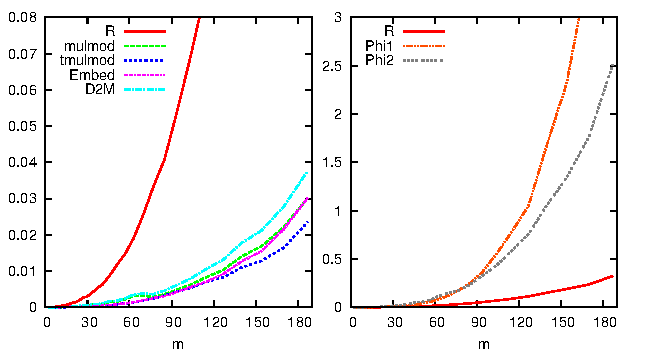
\includegraphics[width = 10cm]{creat}
	\caption{Timings in seconds, $p=5$, $n=m+1$}
	\label{fig:bench}
\end{figure}

Unsurprisingly, the isomorphism algorithms take significantly more
time than the computation of $R$; for our choices of degrees, {\sf
  Phi2} is asymptotically faster than {\sf Phi1} and the crossover
between them happens around $m=70$. 

We compare our implementation to four different strategies available
in Magma. For each of them we measure the time to construct the finite
fields and embedding data, as well as the time to do operations
equivalent to {\sf Embed}, resp.\ inverse
isomorphism. 

Figure~\ref{fig:magma} reports on the following experiments.
In {\sf irred}, we supply directly $P$, $Q$ and $R$ to Magma's
  finite field constructor, then we call the \verb+Embed+ routine to
  compute the embedding data.
 In  {\sf P R}, we use Magma's default constructor to compute $P$
  and $R$ (Magma chooses its own polynomials), then we call the
  \verb+Embed+ routine to compute the embedding.
 In {\sf P Q}, we use Magma's default constructor to compute $P$
  and $Q$ (Magma chooses its own polynomials), then use the
  \verb+CommonOverfield+ routine to compute $R$, then \verb+Embed+ to
  compute the embedding data.
 In {\sf ext}, we use Magma's default constructor to compute $P$,
  then the \verb+ext+ operator to compute an extension of degree $n$
  of $\F_p[x]/\ang{P}$ (Magma chooses its own polynomials).

\begin{figure}
	\centering
	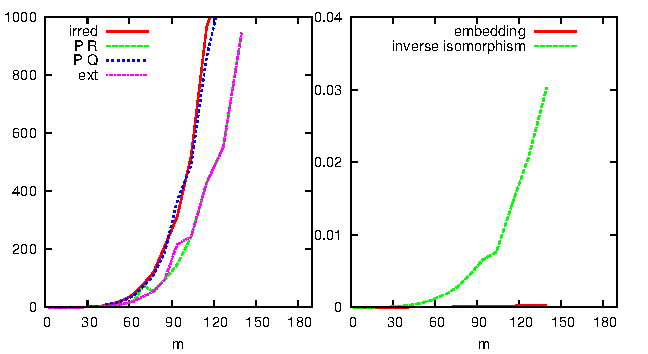
\includegraphics[width = 10cm]{magma}
	\caption{Magma timings in seconds, $p=5$, $n=m+1$}
	\label{fig:magma}
\end{figure}

Timings for constructing the extension and the embedding vary from one
method to the other; once this is done, timings for applying
embeddings or (inverse) isomorphisms are the same across these
methods.

The Magma implementation cannot construct the embedding data in large
cases ($m = 150$) in less than 1000 seconds, while our code takes a
few seconds. Once the embedding data is known, Magma can apply the
embeddings or isomorphisms extremely fast; in our case, one may do the
same, using our algorithms to compute the matrices of $\Phi$ and
$\Phi^{-1}$, when precomputation time and memory are not a concern.

\paragraph{Acknowledgements.} We would like to thank the referees
for their insightful remarks. Part of this work was financed by NSERC,
the CRC program and the ANR project ECLIPSES (ANR-09-VERS-018).

\bibliographystyle{plain}
\bibliography{references}
	
\addcontentsline{toc}{chapter}{Conclusion}

\vspace*{2in}
\begin{center}
	\large
	\textbf{Conclusion}
\end{center}
\vspace*{1cm}

We have presented algorithms to construct and perform computations in algebraic closures of finite 
fields. Most of our algorithms are quasi-linear in the degree of the extension. Experiments show 
that our algorithms and implementations, which use monomial representation, are superior to 
those based on linear algebra. Future directions of this work would include: (i) Designing more 
efficient algorithms for computing isomorphisms, and (ii) Making the construction of towers 
quasi-linear in all cases.
 

	\appendix
	\graphicspath{{finite_fields/}}


\chapter{Finite Fields}
\label{appendix:finite_fields}

In this appendix, we briefly review the theory of finite fields\footnote{We assume the reader has 
a very basic knowledge of some algebraic objects like Groups, Rings, and Ideals.}. A field $K$ is 
a set equipped with two operations $+ : K \times K \rightarrow K$, and $\times : K \times K 
\rightarrow K$ called addition and multiplication. The following conditions are imposed 
for all $a, b, c \in K$:
\begin{enumerate}
	\setlength\itemsep{0mm}
	\item Associativity: $a \times (b \times c) = (a \times b) \times c, a + (b + c) = (a + b) + c$
	\item Commutativity: $a \times b = b \times a, a + b = b + a$
	\item Identity: there exist elements denoted by $0, 1$ in $K$ such that $a \times 1 = a$, and 
	$a + 0 = a$.
	\item Inverse: for $a \ne 0$, there exist $-a, a^{-1} \in K$ such that $a + (-a) = 0$, and $a 
	\times a^{-1} =	1$.
	\item Distributivity: $a \times (b + c) = a \times b + a \times c$.
\end{enumerate}
We usually use familiar notations for the above two operations, e.g. the multiplication symbol is
often skipped. It is apparent from the above conditions that the elements $K^* = K \backslash 0$ 
form a multiplicative group. The multiplicative order of an element $a \in K$ is a the smallest 
positive integer $n$ (if exists) such that $a^n = 1$. The characteristic of a field $K$, denoted 
by $\fieldchar(K)$, is the smallest positive integer $n$ (if exists) such that
\[ \underbrace{1 + \cdots + 1}_{n \text{ times}} = 0. \]
If such integer does not exists, the characteristic is $\infty$. For any field $K$, 
$\fieldchar(K)$ is either $\infty$ or a prime number. A homomorphism $\varphi: E \rightarrow F$ of 
fields is a homomorphism of $E, F$ considered as rings. It preserves addition and multiplication. 
More precisely, $\varphi(ab) = \varphi(a)\varphi(b)$, and $\varphi(a + b) = \varphi(a) + 
\varphi(b)$ for $a, b \in E$.

\paragraph{Polynomial ring.} Given a ring $R$, the set of univariate polynomial with coefficients 
in $R$ is a ring denoted by $R[X]$. The ring of bivariate polynomials is defined by $R[X, Y] = 
R[X][Y]$, and polynomial rings with higher number of variables are defined inductively. When $R$ is 
a field $K$ then every ideal of $K[X]$ is of the form $\ang{f}$, i.e. it is generated by a 
polynomial $f \in K[X]$. A polynomial $f \in K[X]$ is irreducible if it cannot be written as $f = 
gh$ with $\deg g, \deg h > 0$. The ideal $\ang{f}$ is prime if and only if the polynomial $f$ is 
irreducible. In that case the quotient $K[X] / \ang{f}$ is a field. An element $a$ in some 
extension $F$ of $K$ is a root of $f \in K[X]$ if $(X - a)$ is a factor of $f$ in $F[X]$ or 
equivalently if $f(a) = 0$. Each term of a polynomial is called a monomial. The monomial of the 
highest degree is called the leading term, and it coefficient is called the leading coefficient. A 
monic polynomial is a polynomial with leading coefficient equal to 1. Over a field every 
polynomial can be made monic by multiplying it by the inverse of its leading coefficient.
\vspace*{3mm}

A \textbf{\textit{finite field}} is a field with a finite number of elements. The most familiar 
finite fields are the prime fields. Given a prime number $p$, a prime finite field, denoted by 
$\F_p$, is a field consisting of numbers $\{0, 1, \dots, p - 1\}$. The operations are done module 
$p$, and $p$ is called the modulus. Any field $K$ with $\fieldchar(K) = p$ contains a copy of 
$\F_p$. In other words, $K$ is a vector space over $\F_p$. This means the cardinality of a finite 
field is always a prime power, namely $p^{[K: \F_p]}$, where $[K: \F_p]$ is the degree of the 
extension $\F_p \subseteq K$.


\section{Basic properties}

Assume a finite field $F$ has a subfield $E \subseteq F$ of size $q$. If the degree of the 
extension $E \subseteq F$ is $n$ then $F$ has $q^n$ elements. Indeed, the elements of $F$ can be 
represented as unique sums $a_1x_1 + a_2x_2 + \cdots + a_nx_n$ where $a_i \in E$ and $\{x_i\}_i$ 
is a basis of $E$ over $F$ as a vector space. We shall denote a finite field of size $q$, where 
$q = p^n$ is a prime power, by $\F_q$. Every element $a \in \F_q$ satisfies $a^q = a$, since the 
multiplicative group $\F_q^*$ has size $q - 1$. In other words, every element of $\F_q$ is a root 
of the polynomial $g(X) = X^q - X \in \F_p[X]$. We say that $\F_q$ is a splitting field of $g(X)$. 
In general, the a splitting field of a polynomial $f$ over a field $K$ is a the smallest field $L 
\supseteq K$ containing all the roots of $f$. Splitting fields always exists, and they are unique 
up to isomorphisms. This yields the following result.
\begin{result}
	For any given prime $p$ and positive integer $n$ there exists a finite field of size $q = 
	p^n$. Any two such finite field are isomorphic to the splitting field of $X^q - X$ over $\F_p$.
\end{result}
Therefore, we can always talk about \textit{the} finite field of a given size. Since 
$\fieldchar(\F_q) = p$ it is easy to check that $(a + b)^p = a^p + b^p$. This yields the famous 
automorphism 
\[
	\begin{array}{lrll}
		\phi_p: & \F_q & \rightarrow & \F_q \\
		& a & \mapsto & a^p
	\end{array}
\]
called \textit{\textbf{Frobenius automorphism}}. Different powers of the Frobenius are defined by 
composition, e.g. $\phi^2 = \phi \circ \phi$. In fact we have a cyclic group $G = \{ 1, \phi, 
\phi^2, \dots, \phi^{n - 1}\}$ of order $n$. This group is called the Galois group of the 
extension $\F_p \subseteq \F_q$, and is denoted by $\gal(\F_q / \F_p)$. For every element $\sigma 
\in G$ there is a subset $F \subseteq \F_q$ such that $\sigma(a) = a$ for all $a \in F$. One can 
check that $F$ is a field. We call $F$ the fixed field of $\sigma$. Similarly, every subgroup of 
$G$ has a fixed field. In fact, it can be shown that there is a one-to-one correspondence between 
the subgroups of $G$ and subfields of $\F_q$. The subgroups of $G$ are unique and correspond to 
the divisors of $n$. This translate, via the above correspondence, to the following result.
\begin{result}
	For ever divisor $m \mid n$ there is exactly one subfield of $\F_q$ of size $p^m$. Conversely, 
	every subfield of $\F_q$ is of size $p^m$ with $m \mid n$.
\end{result}
Let $K$ be an arbitrary field, and let $G \subseteq K^*$ be a finite subgroup of size $n$. Let $a 
\in G$ be an element with maximal order $m$. Then the order of every other element divides $m$. In 
fact, if $m_1 > 1$ is the order of an element $b \in G$, and $m_1$ is coprime to $m$ then $ab$ has 
order $m_1m > m$ which contradict the assumption of maximality of $m$. Therefore, every element of 
$G$ is a root of $g(X) = X^m - 1$. Since, over a field, $g(X)$ can have at most $m$ roots we have 
$m = n$. So we have found a generator for $G$, hence $G$ is cyclic.
\begin{result}
	The multiplicative group $\F_q^*$ is cyclic.
\end{result}
A generator of the group $\F_q^*$ is called a primitive element of $\F_q$. If $a \in \F_q$ is a 
primitive element then $a^r$ is also a primitive element for all $r$ coprime to $q - 1$. 
Therefore, $\F_q$ has exactly $\varphi(q - 1)$ primitive elements, where $\varphi$ is the Euler's 
totient function. 


\section{Irreducible polynomials}

Let $F \subseteq E$ be an extension of finite fields. We say that the extension is algebraic if 
for every element $a \in E$ there exists a polynomial $g$ over $F$ such that $g(a) = 0$. We define 
the \textit{\textbf{minimal polynomial}} of an element $a \in E$ to be a monic polynomial $g$ over 
$F$ of minimal degree with $g(a) = 0$. The minimality condition on the degree implies that minimal 
polynomials are always irreducible. Indeed, if $g = h_1h_2$ with $\deg h_1, \deg h_2 > 0$ then 
$g(a) = h_1(a)h_2(a) = 0$, and hence say $h_1(a) = 0$ with $\deg h_1 < \deg g$ which is a 
contradiction. 

Another way of introducing minimal polynomials is as follows. As mentioned before, 
every ideal in $F[X]$ can be written as $\ang{f}$ for some $f \in F[X]$. This is, in fact, the 
result of $F[X]$ being an Euclidean domain; i.e. for every $a, b \in F[X]$ with $g \ne 0$, there 
are $q, r \in F[X]$ such that $a = bq + r$ and either $r = 0$ or $\deg r < \deg b$. Let $I \subset 
F[X]$ be an ideal, and let $f \in I$ be a polynomial with lowest degree. We can assume that $f$ is 
monic. Given $g \in F[X]$ we can write $g = fq + r$. If $r \ne 0$ then $r$ then $r = g = fq \in I$ 
and it has a lower degree than $f$ a contradiction. Therefore, $f$ divides every polynomial in 
$I$, and hence $I = \ang{f}$. Now, given $a \in E$ let $I$ be the set of all $g \in F[X]$ such 
that $g(a) = 0$. One readily checks that $I$ is an ideal. Write $I = \ang{f}$, and define $f$ as 
the minimal polynomial of $a$. From this we see that minimal polynomials are unique. It is easy to 
check that the above two definitions are equivalent. The latter yields the following result.
\begin{result}
	Let $F \subseteq E$ be finite field extensions, and let $f \in F[X]$ be the minimal polynomial 
	of an element $a \in E$. Then for any $g \in F[X]$ we have $g(a) = 0$ if and only if $f \mid g$.
\end{result}
One of the interesting polynomials over $\F_q$ is $g(X) = X^{q^r} - X$ for a given $r > 0$. Suppose 
that an irreducible polynomial $f \in \F_q[X]$ of degree $m$ divides this polynomial. The the two 
polynomials have a common root $a$ in the splitting field of $f$ over $\F_q$. Since $a^{q^r} = a$ 
we have the extensions $\F_q \subseteq \F_{q^m} \subseteq \F_q^r$ hence $m \mid r$. Conversely, if 
$m \mid r$ then we have the above extensions and $\F_{q^m}$ is the splitting field of $f$. So $f$ 
and $g$ have a common root $a \in \F_{q^r}$. But $f$ is the minimal polynomial of $a$ over $\F_q$ 
hence $f \mid g$. So we have proved the following. 
\begin{result}
	Let $f$ be an irreducible polynomial of degree $m$ over $\F_q$, and let $g(X) = X^{q^r} - X$. 
	Then $f \mid g$ if and only if $m \mid r$.
\end{result}
The above result say that for a given $r > 0$, $g$ is a the product of all irreducible polynomials 
who's degrees divide $r$. An immediate application of this result is testing for irreducibility. A 
polynomial $f$ of degree $m$ is irreducible if and only if
\begin{enumerate}
	\setlength\itemsep{0mm}
	\item[i]. $f$ divides $X^{q^m} - X$,
	\item[ii]. $\gcd(X^{q^{m / t}} - X, f) = 1$ for all prime divisors $t$ of $m$.
\end{enumerate}
An interesting observation about irreducible polynomials over finite fields is that any extension 
containing one root of an irreducible polynomial contains all the other roots as well. More 
precisely, if $f(X) = X^m + a_{m - 1}X^{m - 1} + \cdots + a_0$ is an irreducible polynomial over 
$\F_q$, and $b \in F_{q^m}$ is a root of $f$ then we have $b^m + a_{m - 1}b^{m - 1} + \cdots + a_0 
= 0$. Raising both sides to the power of $q^i$ for any $1 \le i \le m - 1$ we get $(b^{q^i})^m + 
a_{m - 1}(b^{q^i})^{m - 1} + \cdots + a_0 = 0$. One checks that the distinct elements $b, b^q, 
\dots, b^{q^{m - 1}}$ are all the roots of $f$. These elements are called the conjugates of $b$. 
More generally, given an extension $\F_q \subseteq \F_{q^m}$, and an element $a \in \F_{q^m}$ we 
define the conjugates of $a$ with respect to $\F_q$ as $a, a^q, \dots, a^{q^{m - 1}}$. The 
terminology comes from the action of the elements of $\gal(\F_{q^m} / \F_q) = \{1, \sigma, 
\sigma^2, \dots, \sigma^{m - 1}\}$, where $\sigma^i(x) = x^{q^i}$, on $a$. From the above we also 
see that $\F_{q^m}$ is the splitting field of $f$ over $\F_q$. Therefore, two irreducible 
polynomials of the same degree have isomorphic splitting fields. 

From the beginning we have implicitly assumed that the Galois group $\gal(\F_{q^m} / \F_q)$, which 
is defined to be the group of all automorphisms $\alpha: \F_{q^m} \rightarrow \F_{q^m}$ over 
$\F_q$, consists only of $\sigma^i$ defined above. This is always the case for finite fields. In 
fact, let $\alpha$ be an arbitrary automorphism of $\F_{q^m}$ over $\F_q$. Also let $\beta$ be a 
primitive element of $\F_{q^m}$, and let $f$ be its minimal polynomial of $\F_q$. So $0 = 
\alpha(f(\beta)) = f(\alpha(\beta))$ hence $\alpha(\beta)$ is also a root of $f$. Since all other 
roots of $f$ are conjugates of $\beta$ we must have $\alpha(\beta) = \beta^{q^i}$ for some $0 \le i 
\le m - 1$. Also since $\beta$ is a primitive element we have $\alpha(a) = a^{q^i}$ for all $a \in 
\F_{q^m}$.

\paragraph{Cyclotomic polynomials.} Let $r$ be a positive integer such that $r \mid q - 1$. Then 
there is an element $\zeta \in \F_q$ of order $r$, namely $g^{(q - 1) / r}$ for some generator $g 
\in \F_q^*$. The element $\zeta$ is called a primitive $r$th root of unity. Also for all $1 \le i 
< r$ coprime to $r$, $\zeta^i$ is also a primitive $r$th root of unity. Define the $r$th Cyclotomic 
polynomial as
\[ \Phi_r(X) = \prod_{\substack{1 \le i < r \\ \gcd(i, r) = 1}}(X - \zeta^i). \]
we obviously have $\deg \Phi_r = \phi(r)$ where $\phi$ is the Euler function. The polynomial 
$\Phi_r$ is square-free by definition. Let $f$ be the minimal polynomial of $\zeta$ over $\F_p$, 
and let $d$ be the order of $p$ in the multiplicative group $\Z / r\Z$. Then we know that $d \mid
\phi(r)$ by group theory. As before, $\zeta^{p^i}$ is also a root of $f$ for all $0 \le i < 
\phi(r)$. But only $d$ of these elements are distinct, namely $A = \{ \zeta, \zeta^{p^1}, \dots, 
\zeta^{p^{d - 1}} \}$. So $f$ has degree $d$. We can repeat the same process for the minimal 
polynomial of an element $\zeta^{p^i}$ not in $A$, and append the next set of distinct powers to 
$A$, and so on. All these minimal polynomials divide $\Phi_r$. This yields the following.
\begin{result}
	Let $r$ be a positive integer such that $r \mid q - 1$, and let $d$ be the order of $q$ in $\Z 
	/ r\Z$. Then $\Phi_r$ factors into $\phi(r) / d$ irreducible polynomials of the same degree $d$.
\end{result}
 

\section{Traces and Norms}

Let $F = \F_q$, and $E = \F_{q^m}$ be an extension of $F$. The trace map from $E$ to $F$ is defined 
as
\[
	\begin{array}{lrll}
		\trace_{E/F}: & E & \rightarrow & F \\
		& a & \mapsto & a + a^q + \cdots + a^{q^{m - 1}}.
	\end{array}
\]
So the trace of an element is simply the sum of its conjugates. One hidden fact in the above 
definition is that the image of the trace is actually contained in $F$. This is a direct 
consequence of the fact that trace is fixed by all $\sigma \in \gal(E/F)$. Indeed, 
\begin{align*}
	\trace_{E/F}(a)^q &= (a + a^q + \cdots + a^{q^{m - 1}})^q \\
	& = a^q + \cdots + a^{q^{m - 1}} + a \\
	& = \trace_{E/F}(a). 
\end{align*}
One can easily check that $\trace_{E/F}$ is a linear map over $F$, or an $F$-linear map, 
considering both $E, F$ as vector spaces over $F$; i.e. 
\[ \trace_{E/F}(a\alpha + b\beta) = a\trace_{E/F}(\alpha) + b\trace_{E/F}(\beta) \quad a, b \in F 
\text{ and } \alpha, \beta \in E. \]
This mean $\trace_{E/F}(a) = ma$ for all $a \in F$. An element $a \in E$ is in the kernel $K$ of 
the trace map if it is a root of the polynomial $X + X^q + \cdots + X^{q^{m - 1}}$. But this 
polynomial has at most $q^{m - 1}$ roots. So $\#K \le q^{m - 1}$ hence the image of $\trace_{E/F}$ 
has size larger than $q$. Therefore, the trace map is surjective.

We saw before that every automorphism of $\F_{q^m}$ is of the form $x \mapsto x^{q^i}$ for some $0 
\le i \le m - 1$. This extends to the case of trace maps as follows. Define $\ell_b(a) = 
\trace_{E/F}(ab)$ for $b \in E$ and all $a \in E$. If $a \ne a'$ then $\ell_a - \ell_{a'} = 
\trace_{E/F}(ab) - \trace_{E/F}(ab) = \trace_{E/F}((a - a')b)$ which is not zero for some $b$ as 
the trace in onto. Therefore, $\ell_a \ne \ell_{a'}$. Also there are only a finite number of 
$F$-linear maps $E \rightarrow F$. In fact, every such linear map is determined by assigning 
elements of a given basis of $E$ to elements of $F$. So there are $q^m$ of such maps. But there are 
the same number of maps $\ell_b$ as well. Therefore, every $F$-linear map $E \rightarrow F$ is of 
the form $\ell_b$ for some $b \in E$.

Let $E, F$ be as above. The norm map from $E$ to $F$ is defined 
as
\[
\begin{array}{lrll}
\norm_{E/F}: & E & \rightarrow & F \\
& a & \mapsto & aa^q \cdots a^{q^{m - 1}} = a^{(q^m - 1) / (q - 1)}.
\end{array}
\]
Again the image of $\norm_{E/F}$ is always in $F$. From the definition we have 
\[ \norm_{E/F}(ab) = \norm_{E/F}(a)\norm_{E/F}(b) \quad a,b \in E. \]
This means that norm is a homomorphism $E^* \rightarrow F^*$ of groups. We also have 
$\norm_{E/F}(a) = a^m$ for all $a \in F$. Like trace, norm is also onto: the kernel of 
$\norm_{E/F}$ is a subset of the roots of the polynomial $X^{(q^m - 1) / (q - 1)}$. So the kernel 
has size smaller than $(q^m - 1) / (q - 1)$ hence the image of the map has size larger 
than $q - 1$. The norm and trace maps are both transitive in the following sense.

\begin{result}
	For a chain of extensions $F \subset K \subset E$ of finite fields
	\[ \trace_{E/F}(a) = \trace_{K/F}(\trace_{E/K}(a)), \quad \norm_{E/F}(a) = 
	\norm_{E/K}(\norm_{K/F}(a)) \]
	for all $a \in E$.
\end{result}

\section{Algebraic closures}

In this section, we discuss the basic concepts of algebraic closures and their construction. We 
will also discuss our computational approach to dealing with algebraic closures of finite fields.

A field $L$ is said to be algebraically closed if every non-constant polynomial in $L[X]$ has a 
root in $L$. This is equivalent to saying that every non-constant polynomial splits into linear 
factors over $L$. An \textit{\textbf{algebraic closure}} of a field $K$, denoted by $\overline{K}$, 
is an algebraic extension of $K$ that is algebraically closed.

Given a field $K$ one can build an algebraically closed filed containing $K$ as 
follows. We first build a field $K_1$ such that every polynomial in $K[X]$ has a root in $K_1$. Let 
$\mathcal{S}$ be the set of all polynomials $f \in K[X]$, and let $\mathcal{X}$ be the set of 
variables $\{X_f\}_{f \in \mathcal{S}}$. So we have introduced a variable for each polynomial. Now 
form the ring $K[\mathcal{X}]$, and let $I \subset K[\mathcal{X}]$ be the ideal generated by all 
the polynomials $f(X_f)$. We claim that $I$ is not the unit ideal. If it is, then there is a finite 
linear combination
\[ g_1f_1(X_{f_1}) + \cdots + g_nf_n(X_{f_n}) = 1, \qquad g_i \in K[\mathcal{X}]. \]
This equation involves only a finite number of variables, say $X_{f_1}, \dots, X_{f_N}$. Therefore, 
rewriting the equation gives
\[ \sum_{i = 1}^n g_i(X_{f_1}, \dots, X_{f_N})f_i(X_{f_i}) = 1. \]  
There exists a finite extension $E$ of $K$ in which each $f_i$ has a root. Let $a_i \in E$ be a 
root of $f_i$. Then substituting $a_i$ for $X_{f_i}$ in the above equation will give $0 = 1$ in 
$E$, which is a contradiction. So a simple application of Zorn's lemma gives $I \subseteq 
\mathfrak{m}$ for some maximal ideal $\mathfrak{m}$ of $K[\mathcal{X}]$. So $K_1 = K[\mathcal{X}] / 
\mathfrak{m}$ is a field containing $K$. Also every polynomial $f \in K[X]$ has a root in $K_1$ by 
construction. Repeating the same process for $K_1$, and so on, we obtain a tower
\[ K = K_0 \subseteq K_1 \subseteq K_2 \subseteq \cdots \]
in which every non-constant polynomial in $K_n[X]$ has a root in $K_{n + 1}$ for all $n \ge 0$. Now 
define $K_\infty$ to be the union of all these extensions. One can easily check that $K_\infty$ is 
a field. Let $f \in K_\infty[X]$. Then the coefficients of $f$ are in $K_n$ for a large enough $n$. 
So $f$ has a root in $K_{n + 1} \subseteq K_\infty$, hence $K_\infty$ is algebraically closed.

So given a field $K$ there is an algebraically closed extension $K \subseteq E$. Define $F 
\subseteq E$ as the union of all subfields of $E$ that are algebraic over $K$. It is easy to check 
that $F$ is algebraic over $K$ and it is algebraically closed. Therefore, $F$ is an algebraic 
closure of $K$. It can be shown that algebraic closures are unique up to isomorphism of fields.

\paragraph{Finite fields.} It is a simpler and more intuitive situation for algebraic closures over 
finite fields. Starting from $\F_p$, we know that every irreducible polynomial $f \in \F_p[X]$ of 
degree $n$ has a root in $\F_{p^n}$. So adapting the above general construction of adding roots of 
polynomials we see that we only need to consider extensions $\F_{p^2}, \F_{p^3}, \F_{p^4}, \dots$. 
From previous sections we know that $\F_{p^m} \subseteq \F_{p^n}$ if and only if $m \mid n$. So,  
there are inclusions $\F_{p^{n_1}} \subseteq \F_{p^{n_1n_2}}$ and $\F_{p^{n_2}} \subseteq 
\F_{p^{n_1n_2}}$ for every $n_1, n_2 > 0$. So the above set of finite fields is partially ordered 
by inclusion, and we can talk about the union of any two finite fields. Then we have 
\[ \overline{\F_p} = \bigcup_{i \ge 1} \F_{p^i}. \]
In fact, let $K = \cup_{i \ge 1} \F_{p^i}$, and let $a \in K$. Then $a \in \F_{p^n}$ for some $n$, 
hence $a$ is algebraic over $\F_p$. Also every irreducible polynomial $f \in K[X]$ has coefficients 
in $\F_{p^n}$ for a large enough $n$. Then $f$ has a root in $\F_{p^n}[X] / \ang{f} \cong 
\F_{p^{mn}} \subseteq K$ where $m = \deg f$.


\bibliographystyle{plain}
\bibliography{references}
% 	\thispagestyle{empty}
\vspace*{1cm}

\begin{center}
	\textbf{VITA}
\end{center}

\begin{center}
	\textbf{Javad Doliskani}\\
	\vspace*{2mm}
	Ontario Research Center for Computer Algebra (ORCCA)\\
	Department of Computer Science, University of Western Ontario\\
	London, Ontario, Canada, N6A 5B7
\end{center}

\textbf{Education}
\vspace*{2mm}
\hrule
\vspace*{2mm}
\begin{tabular}{ll}
	2003-2008 & Tarbiat Moallem University, \\
	& Tehran, Tehran, Iran,\\
	& Software Engineering, B.S. \\
	& \\
	2009-2011 & University of Western Ontario, \\
	& London, Ontario, Canada, \\
	& Computer Algebra, MSc. \\
	& \\
	2011-2015 & University of Western Ontario, \\
	& London, Ontario, Canada, \\
	& Computer Algebra, PhD.
\end{tabular}

\end{document}
